\documentclass[12pt,a4paper]{article}
\usepackage[utf8]{inputenc}
\usepackage[T1]{fontenc}
\usepackage[italian]{babel}
\usepackage{libertinus}
\usepackage{amssymb}
\usepackage[a4paper,top=25mm,bottom=25mm,left=22mm,right=22mm,headheight=15pt]{geometry}
\usepackage{graphicx}
\usepackage[table]{xcolor}
\usepackage{tabularx,array,longtable}
\usepackage{float}
\usepackage[font=small,labelfont=bf]{caption}
\usepackage{titlesec}
\usepackage{titletoc}
\usepackage{microtype}
\usepackage{fancyhdr}
\usepackage{enumitem}
\usepackage[hidelinks]{hyperref}

\definecolor{bfblue}{HTML}{1B3F9E}
\definecolor{bfrow}{HTML}{F2F5FC}
\definecolor{bfline}{HTML}{C9D1E6}
\definecolor{bfhead}{HTML}{2E6BE6}
% Segnaposto ancora da compilare (in rosso)
\newcommand{\ph}[1]{\textcolor{red}{[#1]}}
\newcommand{\tightlist}{\setlength{\itemsep}{1pt}\setlength{\parskip}{0pt}}
% Termine presente nel Glossario
\newcommand{\gl}[1]{\emph{#1}\textsubscript{\scriptsize G}}
\setlist{topsep=2pt}
\setlist[itemize]{leftmargin=1.3em,label=\textbullet}
\setlist[enumerate]{leftmargin=1.6em}
\setlength{\parindent}{0pt}
\sloppy
\setlength{\emergencystretch}{2em}
\setlength{\parskip}{5pt}
\renewcommand{\arraystretch}{1.45}
\setcounter{secnumdepth}{3}
\setcounter{tocdepth}{3}

\titleformat{\section}{\LARGE\bfseries\color{bfblue}\raggedright}{\thesection.}{0.3em}{}[{\color{bfblue}\vspace{-2pt}\titlerule[0.9pt]}]
\titleformat{\subsection}{\Large\bfseries\color{bfblue}\raggedright}{\thesubsection.}{0.3em}{}
\titleformat{\subsubsection}{\normalsize\bfseries\raggedright}{\thesubsubsection.}{0.3em}{}
\titleformat{\paragraph}[hang]{\normalsize\bfseries\itshape\raggedright}{}{0em}{}
\titlespacing*{\section}{0pt}{14pt}{6pt}
\titlespacing*{\subsection}{0pt}{10pt}{4pt}
\titlespacing*{\subsubsection}{0pt}{10pt}{3pt}
\titlespacing*{\paragraph}{0pt}{8pt}{2pt}

% Indice: numeri con punto, trattini fino al numero di pagina
\contentsmargin{2.2em}
\newcommand{\bfleader}{\titlerule*[0.32em]{\textendash}}
\titlecontents{section}[0pt]{\addvspace{5pt}\large\bfseries}{\thecontentslabel.\ }{}{\hspace{0.4em}\bfleader\contentspage}
\titlecontents{subsection}[1.2em]{\addvspace{0pt}}{\thecontentslabel.\ }{}{\hspace{0.4em}\bfleader\contentspage}
\titlecontents{subsubsection}[2.4em]{\addvspace{0pt}}{\thecontentslabel.\ }{}{\hspace{0.4em}\bfleader\contentspage}
\titlecontents{figure}[0pt]{\addvspace{0pt}}{Figura \thecontentslabel:\ }{}{\hspace{0.4em}\bfleader\contentspage}

\pagestyle{fancy}
\fancyhf{}
\fancyhead[L]{\footnotesize\sffamily\bfseries\color{bfhead}\textls[120]{BENDING FORKS}}
\fancyhead[R]{\footnotesize\sffamily Analisi dei requisiti}
\fancyfoot[C]{\small Pagina \thepage}
\renewcommand{\headrulewidth}{0.9pt}

% Tabelle: righe alternate e intestazione blu
\newcommand{\bftable}{\rowcolors{2}{bfrow}{white}}
\usepackage{etoolbox}
\AtBeginEnvironment{tabularx}{\bftable}
\AtBeginEnvironment{longtable}{\bftable}
\setlength{\LTpre}{6pt}
\setlength{\LTpost}{6pt}
\usepackage{needspace}
\pretocmd{\section}{\Needspace*{12\baselineskip}}{}{}
\pretocmd{\subsubsection}{\Needspace*{6\baselineskip}}{}{}
\graphicspath{{../assets/}}
\newcommand{\thc}[1]{\textcolor{white}{\textbf{#1}}}
\newcommand{\rl}{\\ \arrayrulecolor{bfline}\hline}

\begin{document}

% ---------- Copertina ----------
\begin{titlepage}
\centering
\vspace*{4mm}

\includegraphics[width=105mm]{logo-bending-forks-trasparente.png}\\[4mm]
\underline{bending.forks.swe@gmail.com}

\vspace{32mm}
{\fontsize{24}{28}\selectfont\bfseries Analisi dei requisiti\par}
\vspace{4mm}
{\large\color{bfblue}\textbf{Capitolato C3: Fossdot -- Smart Speaker Open Source}\par}

\vfill
\begin{tabular}[t]{r|l}
\textbf{Versione} & 0.3.1 \\
\textbf{Tipo} & Documento esterno \\
\textbf{Destinatari} & \emph{Uranion EMEA LTD} \\
 & \emph{Prof. Tullio Vardanega} \\
 & \emph{Prof. Riccardo Cardin} \\
\end{tabular}

\vspace{12mm}
{\large\emph{\textbf{Abstract dei contenuti:}}}\\[1mm]
\begin{minipage}{150mm}\centering Attori, casi d'uso e requisiti del prodotto \emph{Fossdot}, ricavati dal capitolato e dagli incontri con l'azienda \emph{Uranion}, con lo schema del sistema, il tracciamento dei requisiti verso le fonti e le questioni ancora aperte.\end{minipage}
\vspace*{6mm}
\end{titlepage}

% ---------- Indice ----------
\vspace*{2mm}
{\fontsize{22}{26}\selectfont\bfseries Indice\par}
\vspace{6mm}
\makeatletter\@starttoc{toc}\makeatother
\newpage

\vspace*{2mm}
{\fontsize{22}{26}\selectfont\bfseries Elenco delle figure\par}
\vspace{6mm}
\makeatletter\@starttoc{lof}\makeatother
\newpage

% ---------- Registro delle versioni ----------
\section{Registro delle versioni}

\begin{longtable}{>{\raggedright\arraybackslash}p{\dimexpr(\linewidth-10\tabcolsep)*110/1000\relax}>{\raggedright\arraybackslash}p{\dimexpr(\linewidth-10\tabcolsep)*150/1000\relax}>{\raggedright\arraybackslash}p{\dimexpr(\linewidth-10\tabcolsep)*170/1000\relax}>{\raggedright\arraybackslash}p{\dimexpr(\linewidth-10\tabcolsep)*170/1000\relax}>{\raggedright\arraybackslash}p{\dimexpr(\linewidth-10\tabcolsep)*400/1000\relax}}
\rowcolor{bfblue}\thc{Versione} & \thc{Data} & \thc{Scriba} & \thc{Verificatore} & \thc{Descrizione} \\
\endfirsthead
\rowcolor{bfblue}\thc{Versione} & \thc{Data} & \thc{Scriba} & \thc{Verificatore} & \thc{Descrizione} \\
\endhead
0.3.1 & 2026-11-23 & Marco Beltrame & \ph{da assegnare} & Casi d'uso allineati al riepilogo dei casi d'uso v2: aggiunte priorità e fase (PoC o MVP) di ogni caso d'uso; tolto UC2.3 e RF-19; interruzione della risposta solo con la \emph{wake word} (UC5, RF-20, RP-3), senza parola ``stop''; UC9 diviso in UC9.1 (tasti) e UC9.2 (voce), con il nuovo RF-33; nuovo UC31.8 (più \emph{provider}); RF-150, RF-151, RF-152, RF-155 e RF-156 obbligatori; schemi aggiornati \rl
0.3.0 & 2026-11-19 & Marco Beltrame & \ph{da assegnare} & Correzioni dopo la riunione interna del 19/11: configurazione del Wi-Fi con \emph{captive portal}; tolto il codice di associazione (il dispositivo nuovo si aggiunge alla casa dalla web app e riceve una credenziale propria); connessione WebSocket sempre aperta e aggiornamenti notificati dal server; aggiunta la lingua inglese; tolto RF-141; contesto gestito solo dall'Amministratore dalla web app e, a voce, solo aggiunte; conferma a voce delle azioni con effetti esterni obbligatoria (RF-142, nuovi UC10.3 e RF-144); RP-4 a 1 s e RP-6 a 15 s; questioni aperte riviste \rl
0.2.0 & 2026-11-19 & Marco Beltrame & \ph{da assegnare} & Unione della v0.1.0 con la bozza di analisi completa del 15/11: perimetro allineato a capitolato e verbali (server di bridging, MCP, Skills e Agents, più dispositivi, case e stanze); tabella degli stati con identificativi; schede dei casi d'uso completate con precondizioni e postcondizioni come stato del sistema, scenari alternativi ed estensioni con punto di innesto; casi d'errore come sottocasi con attore primario umano; colonna del metodo di verifica nei requisiti; riferimenti con versione \rl
0.1.0 & 2026-11-18 & Matteo Wu, Luca Stangherlin & Nicholas Salmaso & Prima stesura del documento \rl
\end{longtable}

% =====================================================================
\section{Introduzione}

\subsection{Scopo del documento}

Il presente documento raccoglie tutto ciò che il capitolato C3 \emph{Fossdot} e gli incontri con l'azienda \emph{Uranion} chiedono al prodotto, e lo organizza in attori, casi d'uso e requisiti collegati a uno schema del sistema. Serve al gruppo come base per la progettazione e alla proponente per confermare che i bisogni sono stati compresi correttamente.

L'Analisi dei requisiti è un documento \textbf{incrementale}: le parti ancora da confermare con la proponente hanno fonte ``Interna'' e sono raccolte nella sezione \ref{sec:aperte}, e verranno aggiornate dopo ogni incontro.

\subsection{Convenzioni}

Il documento segue le convenzioni delle Norme di progetto:
\begin{itemize}
\tightlist
\item \textbf{casi d'uso}: \texttt{UC[Numero].[Sottocaso] -- [Titolo]}, dove le parentesi quadre indicano i campi da sostituire: ad esempio \texttt{UC2 -- Richiesta vocale con risposta} e \texttt{UC2.1 -- Acquisizione della richiesta e rilevamento della fine};
\item \textbf{requisiti}: \texttt{R[Tipo]-[Numero]-[Priorità]}, ad esempio \texttt{RF-1-Obb}.
\end{itemize}
Il tipo è \texttt{F} (funzionale), \texttt{Q} (di qualità), \texttt{V} (di vincolo) o \texttt{P} (prestazionale); la priorità è \texttt{Obb} (obbligatorio), \texttt{Des} (desiderabile) o \texttt{Opz} (opzionale). I numeri dei requisiti funzionali sono raggruppati per area (ad esempio da RF-40 per l'\emph{onboarding}, da RF-100 per i \emph{provider} AI): i salti nella numerazione sono voluti e lasciano spazio a nuovi requisiti senza rinumerare quelli esistenti.

\subsubsection{Metodo di verifica}

Ogni requisito indica come si accerta che sia soddisfatto. I casi di prova corrispondenti saranno descritti nel Piano di qualifica.

\begin{center}
\begin{tabularx}{\linewidth}{>{\raggedright\arraybackslash}p{1.6cm}X}
\rowcolor{bfblue}\thc{Sigla} & \thc{Metodo} \\
T & \textbf{Test}: prova ripetibile, automatica o manuale, con esito misurabile \rl
D & \textbf{Dimostrazione}: esecuzione osservata della funzione sul prodotto, ad esempio durante la revisione con la proponente \rl
I & \textbf{Ispezione}: esame di codice, documentazione, configurazione o \emph{hardware} \rl
A & \textbf{Analisi}: calcolo, misura aggregata o stima a partire da dati raccolti (ad esempio i report della CI) \rl
\end{tabularx}
\end{center}

\subsubsection{Fonti}

Ogni requisito indica la propria fonte, come previsto dalle Norme di progetto. Le fonti sono indicate in questo modo:

\begin{center}
\begin{tabularx}{\linewidth}{>{\raggedright\arraybackslash}p{3.2cm}X}
\rowcolor{bfblue}\thc{Fonte} & \thc{Significato} \\
Capitolato & Capitolato d'appalto C3 \emph{Fossdot} e relativa presentazione \rl
VE \emph{gg/mm} & Verbale esterno dell'incontro con \emph{Uranion} nella data indicata \rl
Interna & Proposta del gruppo, da confermare con la proponente \rl
UC\emph{n} & Requisito ricavato dal caso d'uso indicato \rl
\end{tabularx}
\end{center}

\subsubsection{Assegnazione della priorità}

\begin{itemize}
\tightlist
\item \textbf{Obb}: richiesto dall'MVP del capitolato oppure indicato da \emph{Uranion} come necessario;
\item \textbf{Des}: richiesto dalla versione completa del capitolato oppure indicato da \emph{Uranion} come gradito ma non obbligatorio;
\item \textbf{Opz}: idea del gruppo o di \emph{Uranion} utile ma non richiesta, oppure funzione che \emph{Uranion} ha messo esplicitamente fuori da questa fase ma per cui vuole l'architettura predisposta.
\end{itemize}

Anche i casi d'uso hanno una priorità (Obb, Des, Opz) e una fase di realizzazione: \emph{PoC} (\emph{Proof of Concept}) oppure \emph{MVP}. Priorità e fase di ogni caso d'uso sono nella sezione \ref{sec:fasi}.

\subsection{Riferimenti}

\subsubsection{Riferimenti normativi}
\begin{itemize}
\tightlist
\item \emph{Norme di progetto}, gruppo Bending Forks, versione \ph{x.y.z};
\item Capitolato d'appalto C3 \emph{Fossdot}, \emph{Uranion EMEA LTD}, Rev.~0.1 del 10/09/2026: \url{https://www.math.unipd.it/~tullio/IS-1/2026/Progetto/C3.pdf} \ph{verificare il link};
\item Regolamento del progetto didattico, Ingegneria del Software 2026/27: \ph{link e data di consultazione}.
\end{itemize}

\subsubsection{Riferimenti informativi}
\begin{itemize}
\tightlist
\item T. Vardanega, \emph{T05 -- Analisi dei requisiti}, slide del corso di Ingegneria del Software: \url{https://www.math.unipd.it/~tullio/IS-1/2025/Dispense/T05.pdf} \ph{aggiornare all'edizione 2026/27};
\item R. Cardin, \emph{Diagrammi dei casi d'uso}, slide del corso: \url{https://www.math.unipd.it/~rcardin/swea/2022/Diagrammi\%20Use\%20Case.pdf};
\item Verbale esterno dell'incontro con \emph{Uranion} del 21/10/2026, versione \ph{x.y.z};
\item Verbale esterno dell'incontro con \emph{Uranion} del 13/11/2026, versione \ph{x.y.z};
\item \emph{Bill of Materials}, gruppo Bending Forks, versione 0.2.0;
\item \emph{Glossario}, gruppo Bending Forks, versione \ph{x.y.z}.
\end{itemize}

\subsection{Glossario}

I termini tecnici usati nel documento sono definiti nel Glossario del gruppo. La sezione \ref{sec:glossario} riporta i principali, per facilitare la lettura alla proponente.

\section{Descrizione del prodotto}

\subsection{Scopo del prodotto}

\emph{Fossdot} è uno smart speaker \emph{open source} sul modello dell'Echo Dot, pensato per chi vuole un assistente vocale rispettoso della privacy e controllabile in ogni sua parte. Gli smart speaker in commercio sono chiusi, legati al \emph{cloud} del produttore e a un unico assistente, e quando il produttore spegne i servizi diventano inutili. \emph{Fossdot} lascia invece al proprietario la scelta del \emph{provider} AI, in \emph{cloud} o in locale, permette di estenderlo con protocolli standard come MCP e fa cooperare più dispositivi in casa (Capitolato).

\subsection{Perimetro}

Il prodotto si compone di quattro parti (Capitolato):

\begin{enumerate}
\tightlist
\item \textbf{Hardware}: scheda audio \emph{reSpeaker XVF3800} (4 microfoni, processore audio \emph{XMOS}, anello di 12 LED), microcontrollore \emph{XIAO ESP32-S3}, altoparlante da 5 W, alimentatore e cavo USB-C, scocca. I componenti e la loro scelta sono descritti nella \emph{Bill of Materials}.
\item \textbf{Firmware del dispositivo}: rileva la \emph{wake word} in locale, invia l'audio al server, riproduce la risposta e dà un riscontro visivo.
\item \textbf{Server di bridging}: riceve l'audio della richiesta dal dispositivo, realizza la \emph{pipeline} STT \textrightarrow{} LLM \textrightarrow{} TTS con un \emph{provider} AI configurabile e, nella versione completa, client MCP, Skills e Agents.
\item \textbf{Web app di gestione}: registrazione degli account, associazione e gestione dei dispositivi, configurazione del \emph{provider}.
\end{enumerate}
\subsection{Fuori perimetro in questa fase}

\begin{longtable}{>{\raggedright\arraybackslash}p{\dimexpr(\linewidth-6\tabcolsep)*379/1000\relax}>{\raggedright\arraybackslash}p{\dimexpr(\linewidth-6\tabcolsep)*483/1000\relax}>{\raggedright\arraybackslash}p{\dimexpr(\linewidth-6\tabcolsep)*138/1000\relax}}
\rowcolor{bfblue}\thc{Elemento} & \thc{Motivo} & \thc{Fonte} \\
\endfirsthead
\rowcolor{bfblue}\thc{Elemento} & \thc{Motivo} & \thc{Fonte} \\
\endhead
\emph{Onboarding} di dispositivi IoT di terze parti (lampade Tuya, Philips) & Fuori perimetro, ma l'architettura delle \emph{skill} deve permetterlo in futuro & VE 21/10 \rl
\emph{Marketplace} pubblico delle \emph{skill} & Fuori scopo; in futuro potrebbe nascere un archivio pubblico & VE 21/10 \rl
App mobile dedicata & Basta una web app \emph{responsive} & VE 21/10 \rl
Riconoscimento di chi sta parlando (\emph{speaker identification}) & Complesso per un ESP32; il contesto si associa al dispositivo & VE 13/11 \rl
Profilazione affidata al \emph{provider} dell'LLM & Esclusa da Uranion & VE 13/11 \rl
\end{longtable}

\section{Descrizione generale e schema del sistema}

\subsection{Mappa dell'analisi}

La mappa riassume in un colpo d'occhio le aree funzionali e i vincoli trattati nel documento.

\begin{figure}[H]
\centering
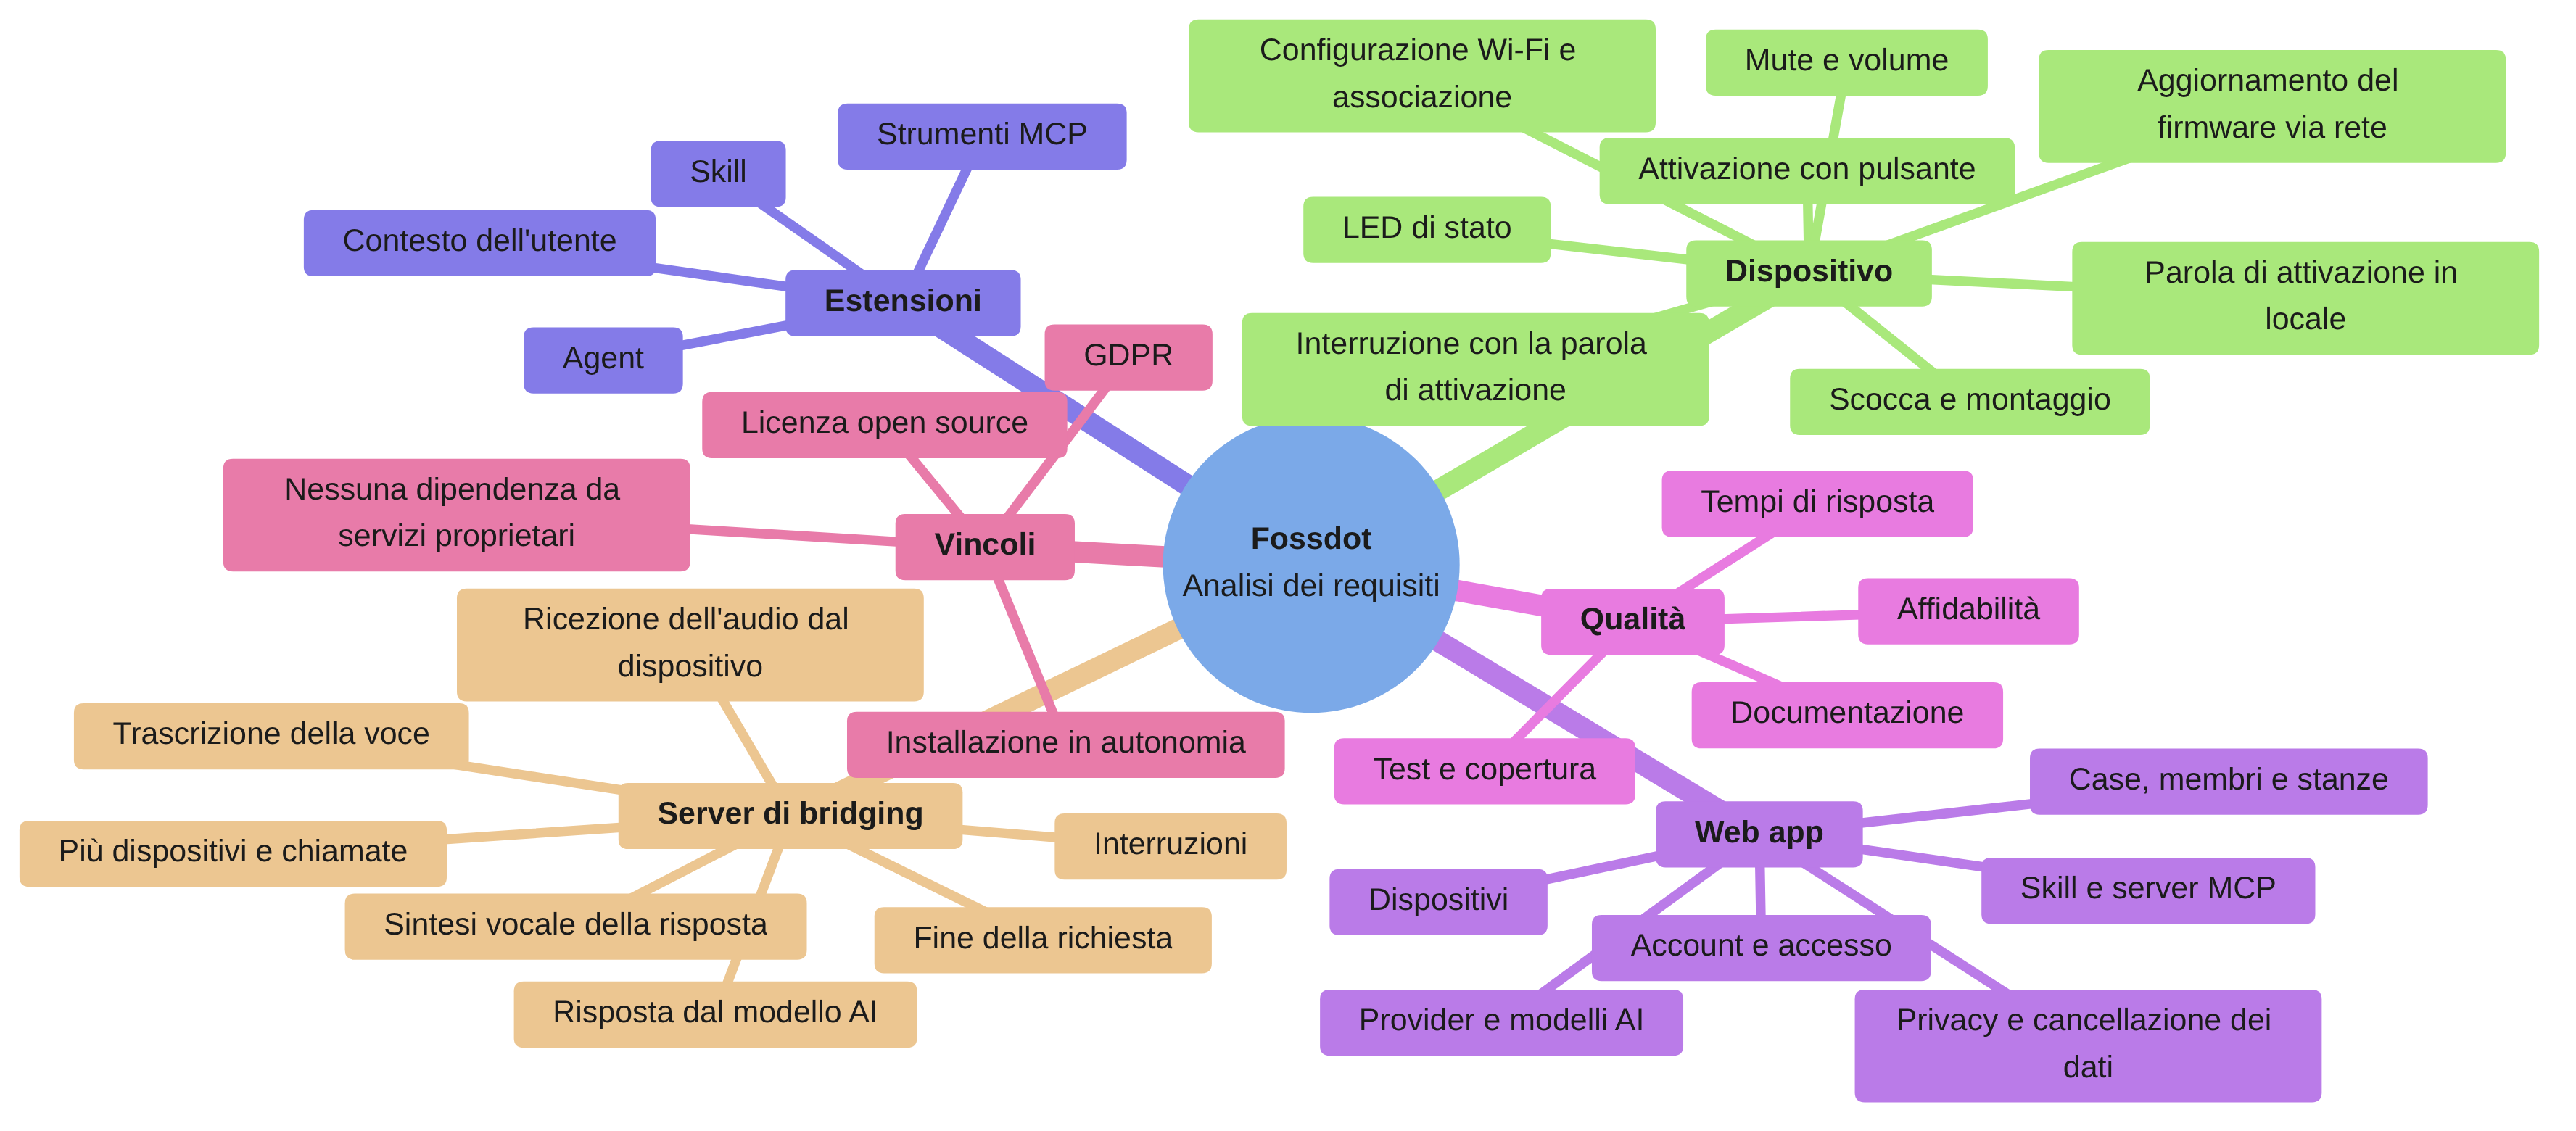
\includegraphics[width=\linewidth,height=0.62\textheight,keepaspectratio]{img_adr/15-mappa.png}
\caption{Mappa delle aree dell'analisi}
\end{figure}

\subsection{Architettura logica}

Il sistema ha tre parti che il gruppo sviluppa (dispositivo, server di bridging, web app) e alcuni servizi esterni che restano sostituibili. Il dispositivo fa poche cose ma le deve fare bene: riconoscere la \emph{wake word}, registrare in modo affidabile, riprodurre la risposta e mostrare lo stato. Tutta l'intelligenza sta sul server, che l'utente installa e controlla (\emph{self-hosted}).

\begin{figure}[H]
\centering
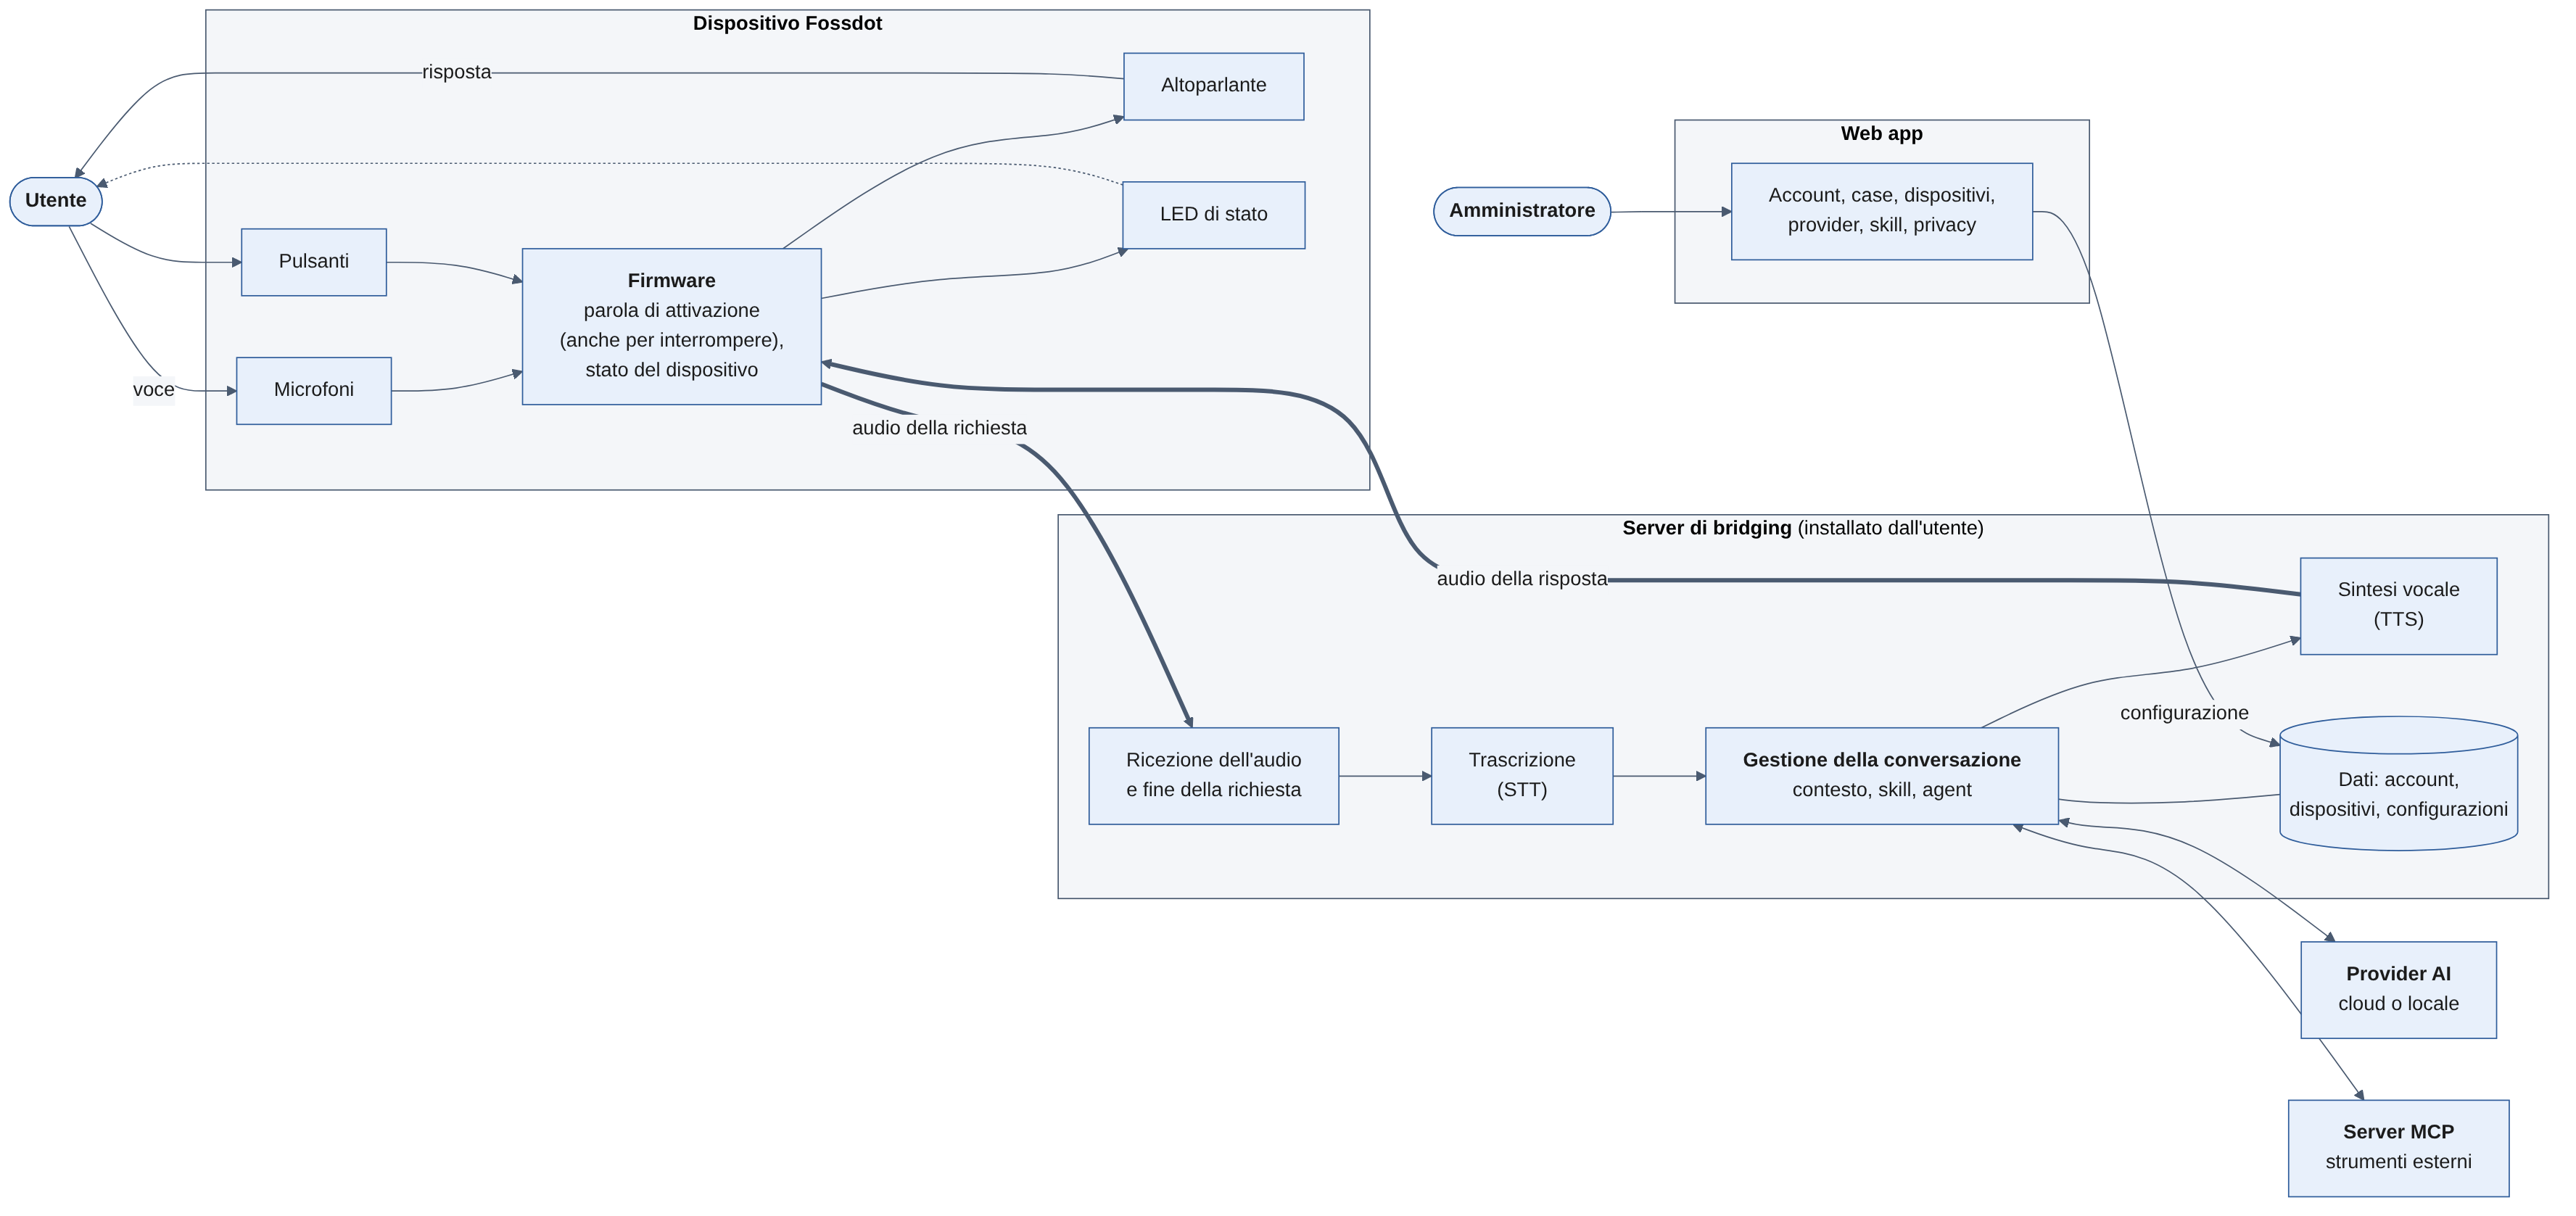
\includegraphics[width=\linewidth,height=0.62\textheight,keepaspectratio]{img_adr/01-architettura.png}
\caption{Architettura logica del sistema}
\end{figure}

Lo schema mostra le tre parti sviluppate dal gruppo. Il \emph{firmware} riconosce in locale la parola di attivazione, anche durante la risposta per interromperla, gestisce lo stato del dispositivo e lo mostra sui LED. Il server di bridging riceve l'audio, lo trascrive, ottiene la risposta dal \emph{provider} AI configurato (eventualmente usando strumenti MCP) e la converte in voce: trascrizione e sintesi vocale fanno parte del server. La web app serve all'Amministratore per configurare il sistema.

\subsection{Flusso principale di una richiesta}

\begin{figure}[H]
\centering
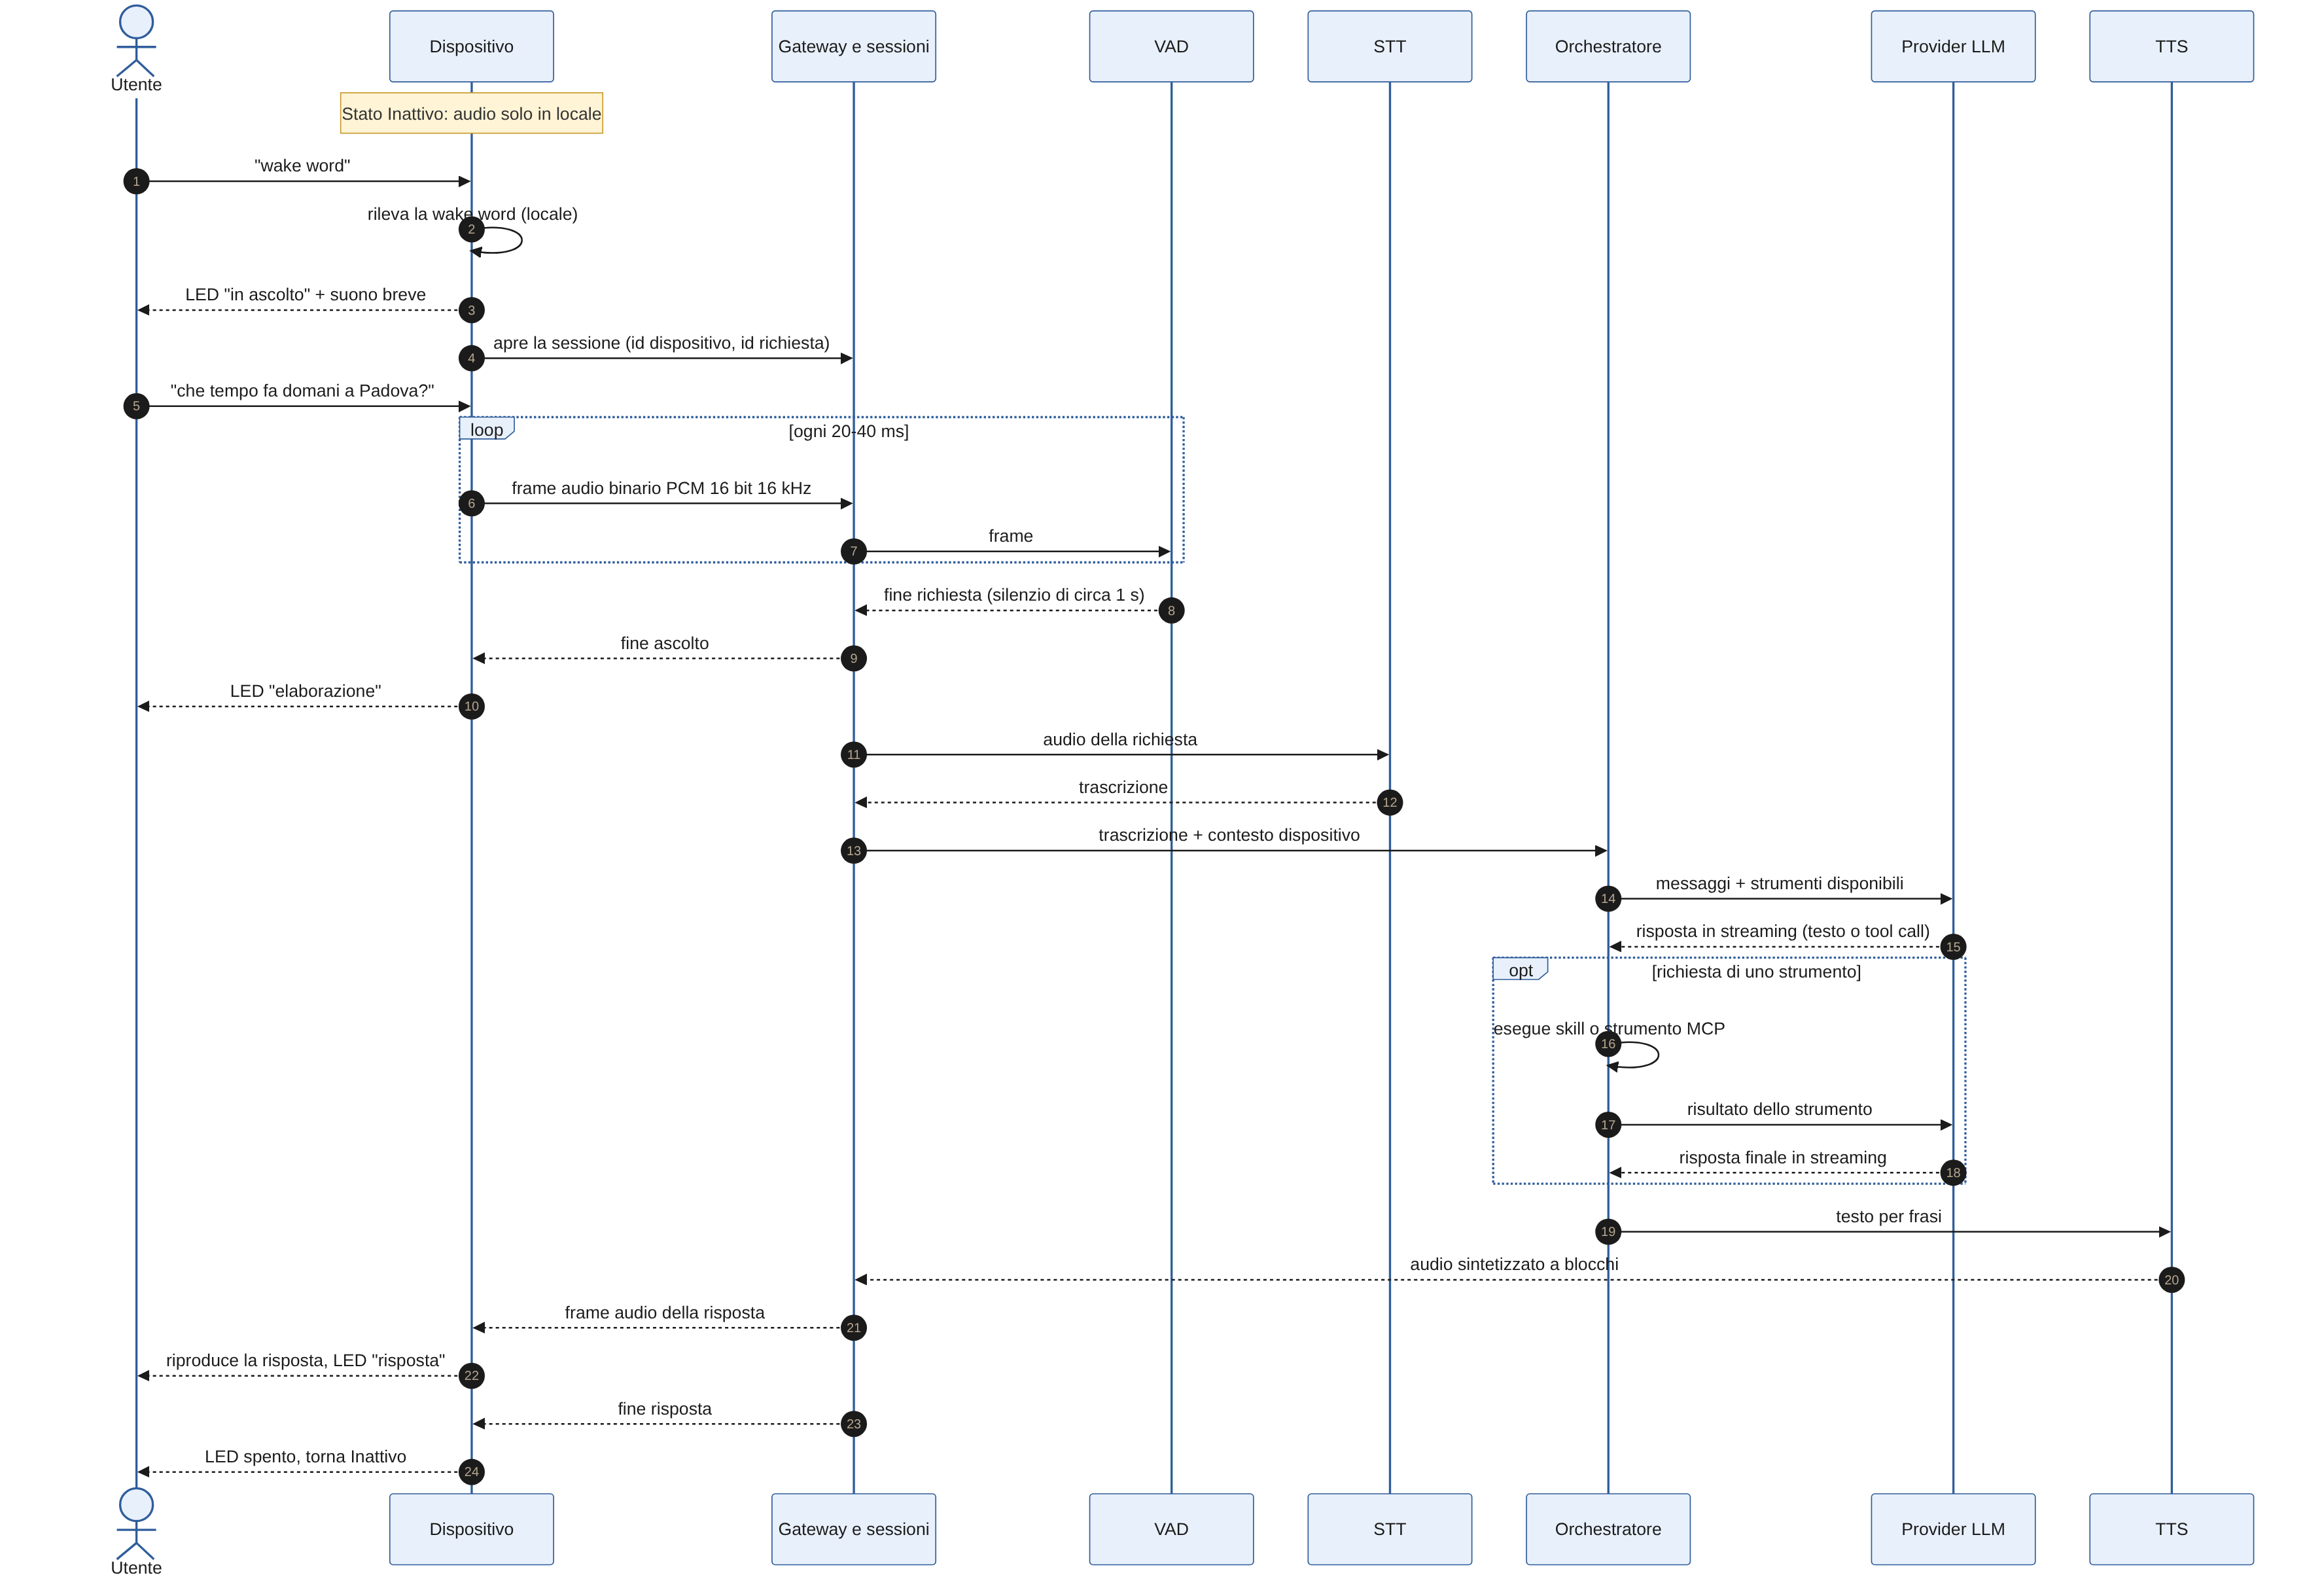
\includegraphics[width=\linewidth,height=0.62\textheight,keepaspectratio]{img_adr/03-sequenza-richiesta.png}
\caption{Sequenza di una richiesta vocale}
\end{figure}

\subsection{Stati del dispositivo}

Il dispositivo è sempre in uno degli stati della tabella \ref{tab:stati}, e ogni stato ha un riscontro visivo sui LED (RF-26). Lo stato composto \emph{Operativo} contiene il ciclo di una richiesta. Le precondizioni e le postcondizioni dei casi d'uso usano gli identificativi della tabella.

\begin{figure}[H]
\centering
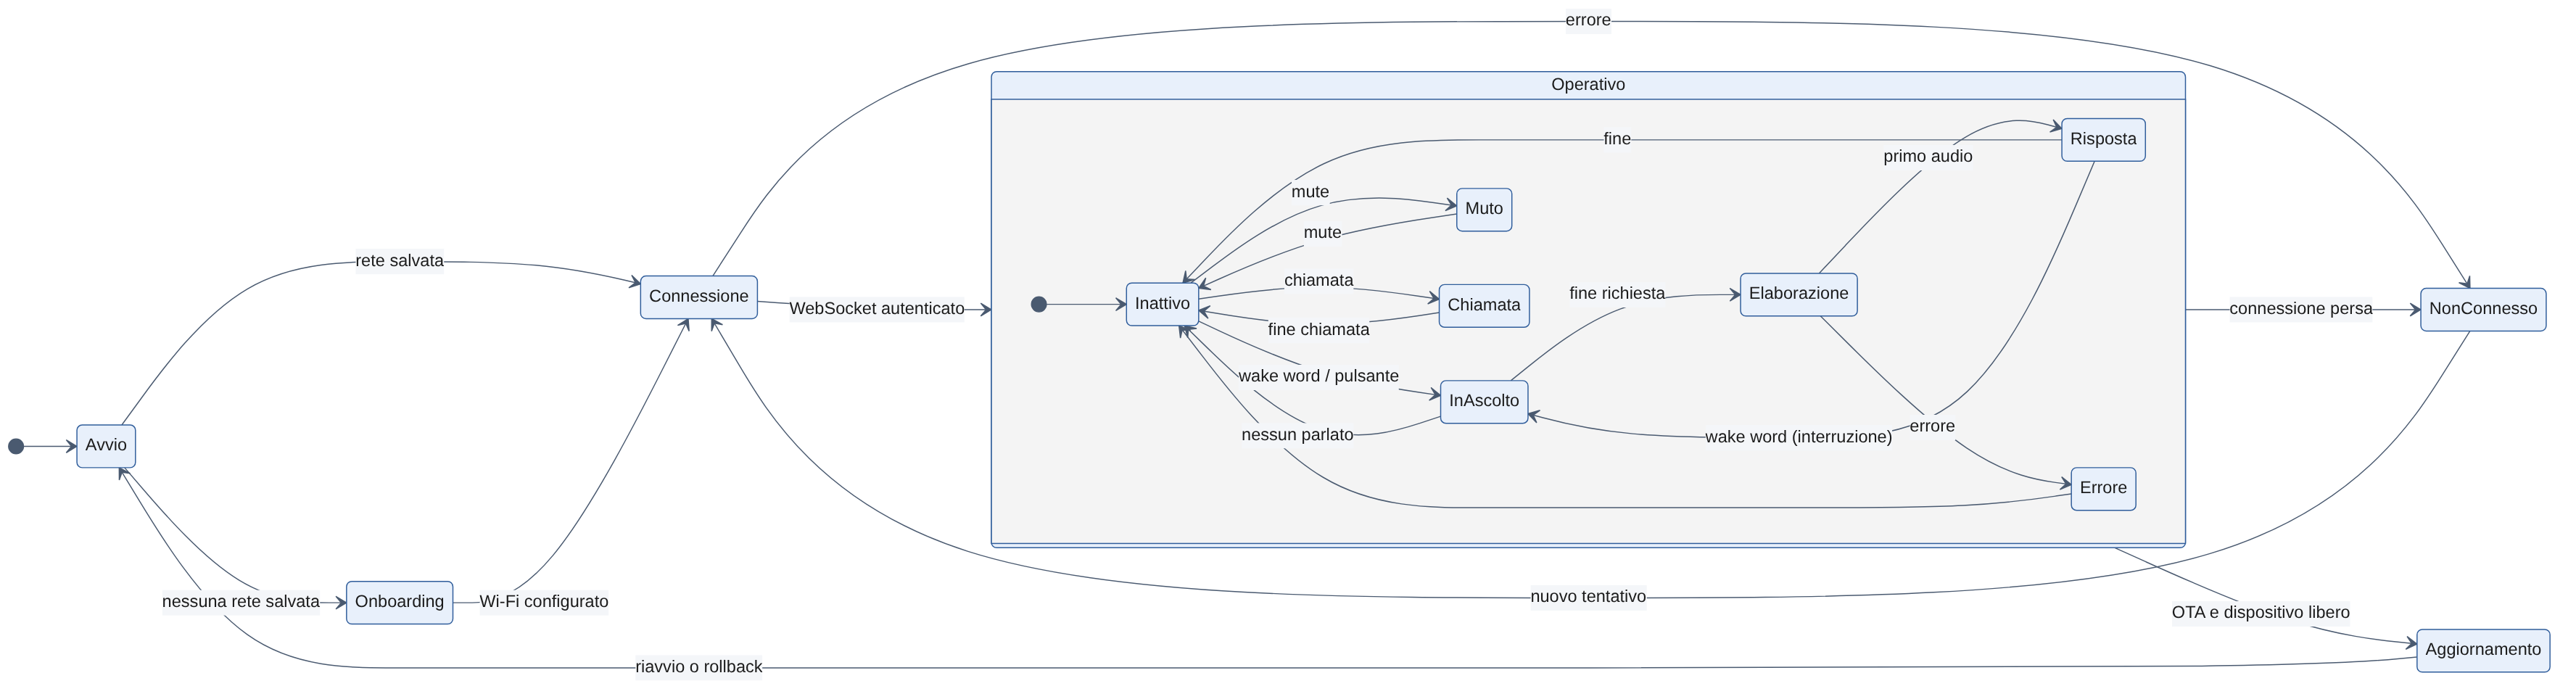
\includegraphics[width=\linewidth,height=0.62\textheight,keepaspectratio]{img_adr/04-stati-dispositivo.png}
\caption{Stati del dispositivo}
\end{figure}


\begin{longtable}{>{\raggedright\arraybackslash}p{\dimexpr(\linewidth-8\tabcolsep)*80/1000\relax}>{\raggedright\arraybackslash}p{\dimexpr(\linewidth-8\tabcolsep)*170/1000\relax}>{\raggedright\arraybackslash}p{\dimexpr(\linewidth-8\tabcolsep)*400/1000\relax}>{\raggedright\arraybackslash}p{\dimexpr(\linewidth-8\tabcolsep)*350/1000\relax}}
\caption{Stati del dispositivo}\label{tab:stati}\\
\rowcolor{bfblue}\thc{ID} & \thc{Stato} & \thc{Descrizione} & \thc{Transizioni in uscita} \\
\endfirsthead
\rowcolor{bfblue}\thc{ID} & \thc{Stato} & \thc{Descrizione} & \thc{Transizioni in uscita} \\
\endhead
ST-1 & Avvio & Il dispositivo si accende e controlla se ha una rete salvata. & rete salvata $\rightarrow$ ST-3; nessuna rete $\rightarrow$ ST-2 \rl
ST-2 & \emph{Onboarding} & Il dispositivo crea una propria rete Wi-Fi temporanea e offre la pagina di configurazione (\emph{captive portal}, UC16); la \emph{wake word} non è attiva. & configurazione riuscita $\rightarrow$ ST-3 \rl
ST-3 & Connessione & Il dispositivo apre la connessione con il server e si autentica con la propria credenziale; un dispositivo nuovo attende di essere aggiunto a una casa (UC17). & connessione autenticata $\rightarrow$ ST-4; errore $\rightarrow$ ST-11 \rl
ST-4 & Inattivo & Ascolto locale della \emph{wake word}; nessun audio lascia il dispositivo (RV-3). & attivazione $\rightarrow$ ST-5; mute $\rightarrow$ ST-8; chiamata $\rightarrow$ ST-9; aggiornamento $\rightarrow$ ST-12; connessione persa $\rightarrow$ ST-11 \rl
ST-5 & In ascolto & Acquisizione della richiesta e invio dell'audio al server (UC2.1). & fine richiesta $\rightarrow$ ST-6; nessun parlato $\rightarrow$ ST-4 \rl
ST-6 & Elaborazione & Il server trascrive, interroga il \emph{provider} ed eventualmente gli strumenti. & primo audio della risposta $\rightarrow$ ST-7; errore $\rightarrow$ ST-10 \rl
ST-7 & Risposta & Riproduzione della risposta in \emph{streaming}. & fine $\rightarrow$ ST-4; \emph{wake word} (UC5, UC6) $\rightarrow$ ST-5 \rl
ST-8 & Muto & I microfoni non acquisiscono audio, nemmeno per la \emph{wake word}. & nuovo comando di mute $\rightarrow$ ST-4 \rl
ST-9 & Chiamata & Audio in tempo reale con un altro dispositivo (UC14). & fine chiamata $\rightarrow$ ST-4 \rl
ST-10 & Errore & Segnalazione di un errore all'utente (UC7). & fine segnalazione $\rightarrow$ ST-4 \rl
ST-11 & Non connesso & Il server non è raggiungibile; il dispositivo ritenta con attese crescenti (RF-48). & nuovo tentativo $\rightarrow$ ST-3 \rl
ST-12 & Aggiornamento & Download, verifica e installazione di un nuovo \emph{firmware} (UC20). & riavvio o ritorno alla versione precedente $\rightarrow$ ST-1 \rl
\end{longtable}

Gli stati ST-4 -- ST-10 formano lo stato composto \emph{Operativo} dello schema. Ogni stato ha un riscontro distinguibile sui LED (RF-26).

\textbf{Fine della richiesta.} Lo schema seguente mostra come il server decide che l'utente ha finito di parlare. I rombi in giallo contengono valori ipotizzati dal gruppo, da tarare con le prove (RP-4, RP-5, RP-6).

\begin{figure}[H]
\centering
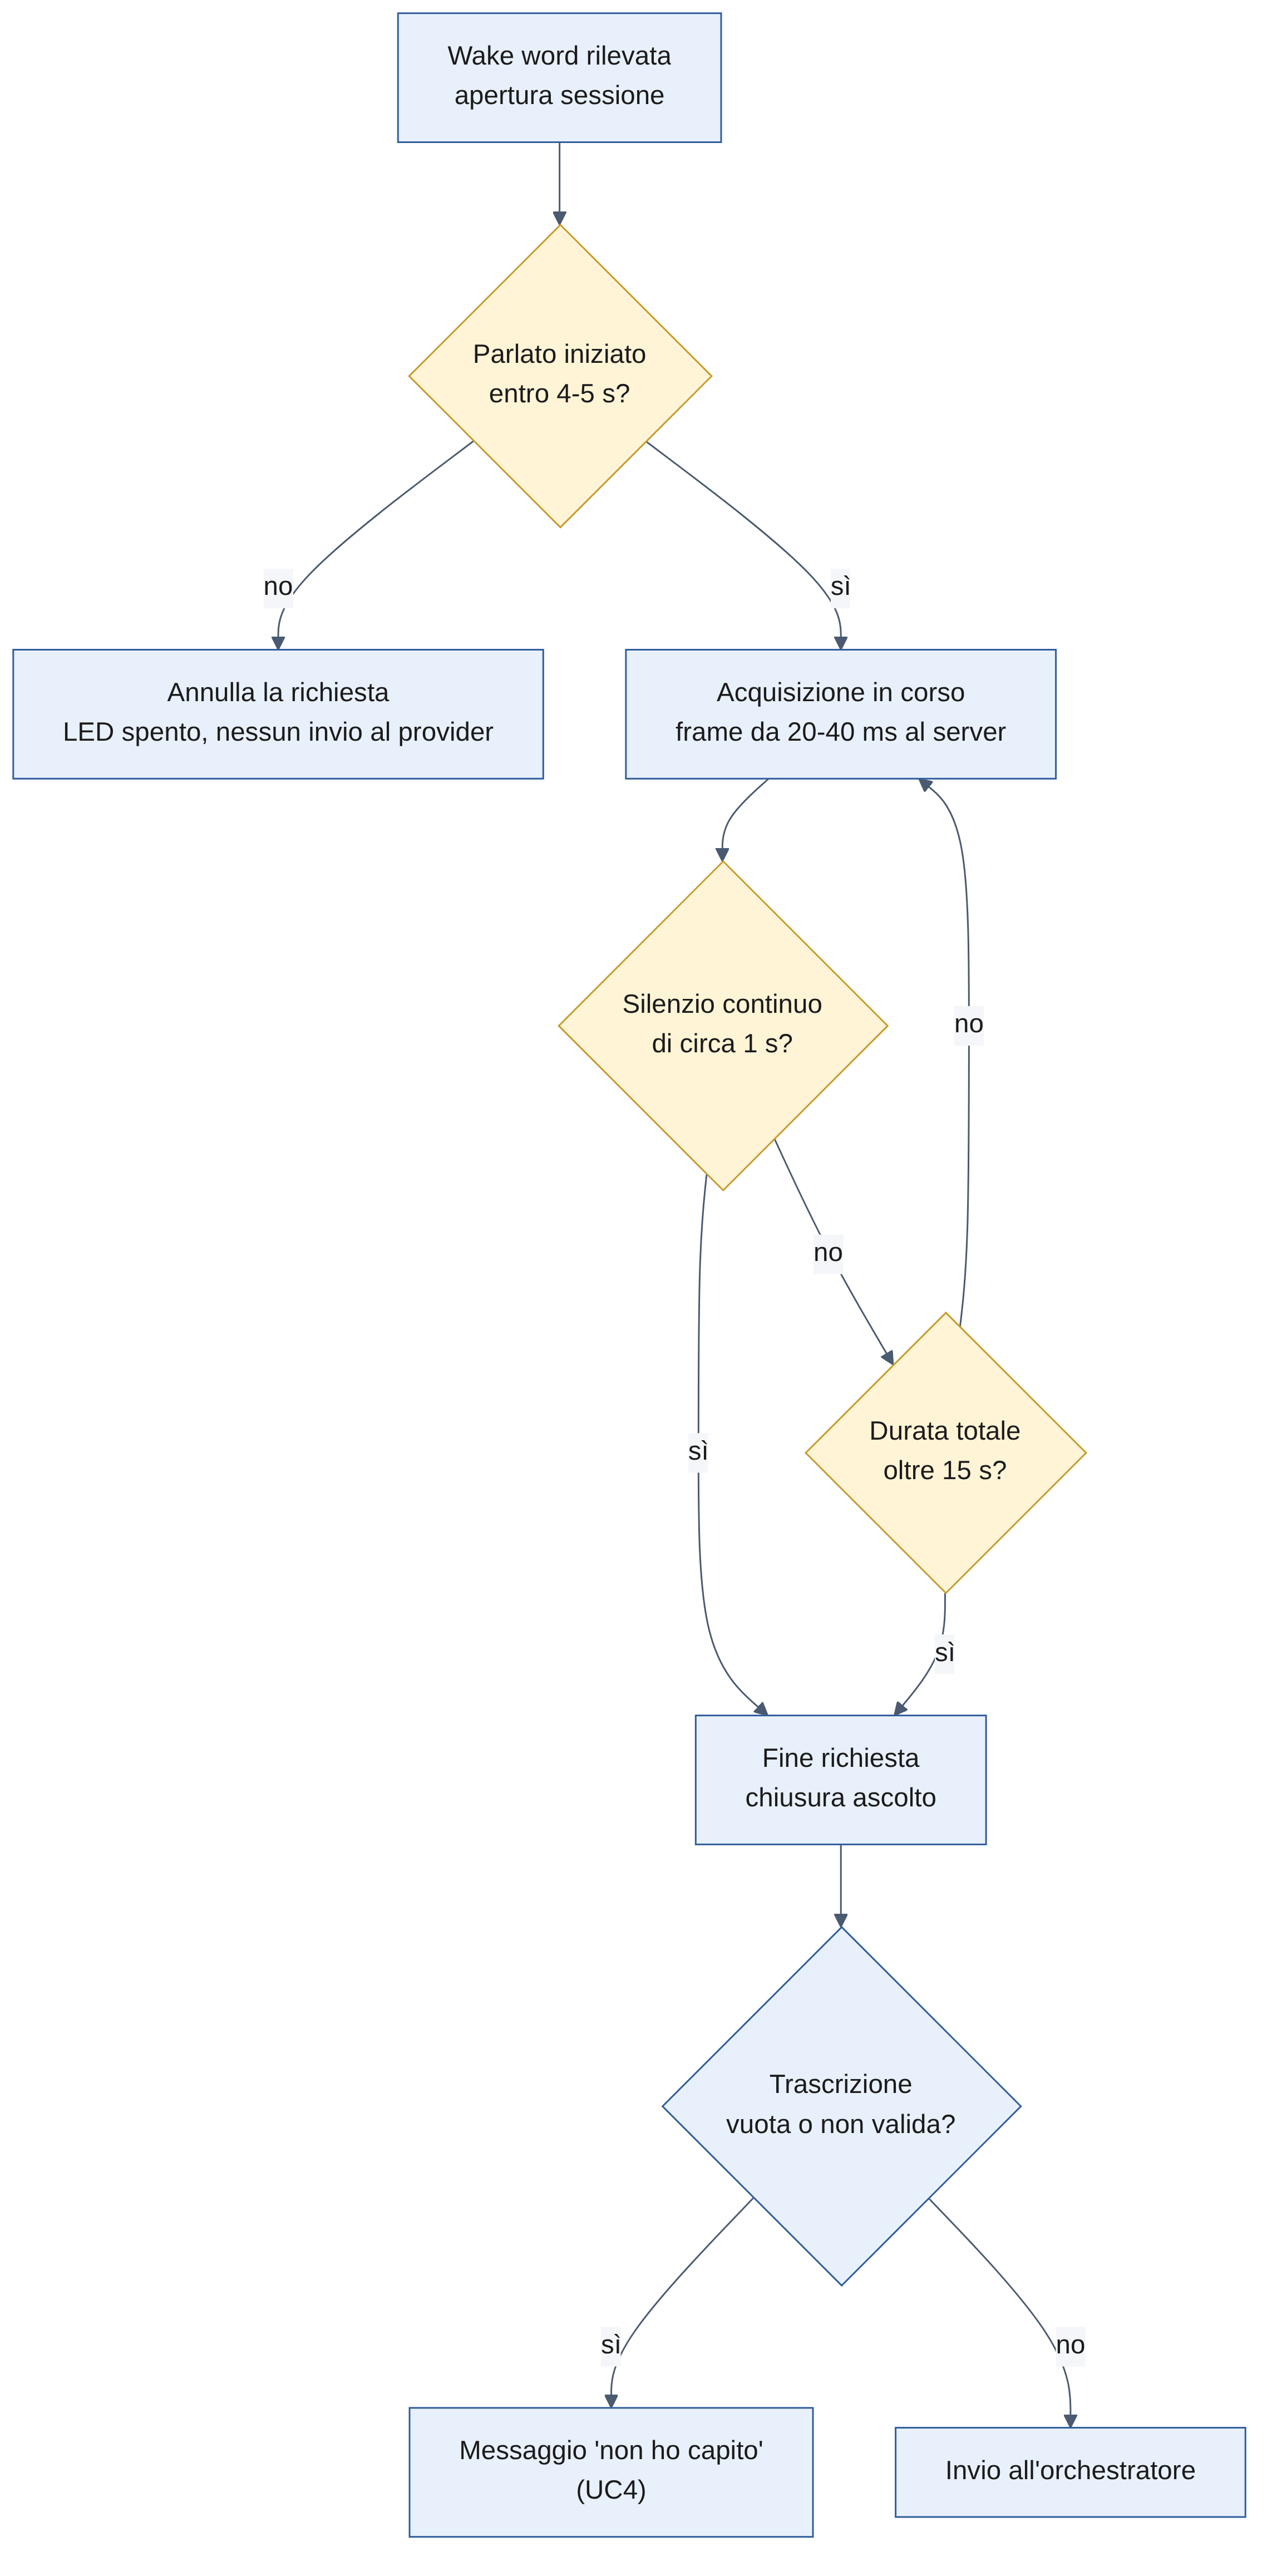
\includegraphics[width=\linewidth,height=0.62\textheight,keepaspectratio]{img_adr/05-fine-richiesta.png}
\caption{Rilevamento della fine della richiesta}
\end{figure}

\section{Attori}

\subsection{Attori primari}

\begin{longtable}{>{\raggedright\arraybackslash}p{\dimexpr(\linewidth-6\tabcolsep)*209/1000\relax}>{\raggedright\arraybackslash}p{\dimexpr(\linewidth-6\tabcolsep)*627/1000\relax}>{\raggedright\arraybackslash}p{\dimexpr(\linewidth-6\tabcolsep)*164/1000\relax}}
\rowcolor{bfblue}\thc{Attore} & \thc{Descrizione} & \thc{Dove interagisce} \\
\endfirsthead
\rowcolor{bfblue}\thc{Attore} & \thc{Descrizione} & \thc{Dove interagisce} \\
\endhead
\textbf{Utente} & Qualsiasi persona che parla al dispositivo. Non deve essere autenticata: il sistema la riconosce solo come ``chi sta parlando a questo dispositivo'' (VE 13/11). & Dispositivo \rl
\textbf{Utente non autenticato} & Persona che apre la web app senza aver effettuato l'accesso. & Web app \rl
\textbf{Membro} & Utente autenticato che appartiene a una casa. Vede i dispositivi e gestisce il proprio profilo e i propri dati; non vede né modifica il contesto dei dispositivi. & Web app \rl
\textbf{Amministratore} & Membro della casa con permessi di gestione: associa e configura i dispositivi, i \emph{provider}, le \emph{skill}, i server MCP e gli altri membri. Chi crea una casa ne è l'Amministratore. È anche chi esegue l'\emph{onboarding} fisico del dispositivo. & Web app, dispositivo \rl
\end{longtable}

Nell'MVP basta un solo account per casa, che è sempre Amministratore. Il ruolo Membro serve quando si gestiscono più utenti (VE 21/10).

\subsection{Attori secondari}

\begin{longtable}{>{\raggedright\arraybackslash}p{\dimexpr(\linewidth-4\tabcolsep)*224/1000\relax}>{\raggedright\arraybackslash}p{\dimexpr(\linewidth-4\tabcolsep)*776/1000\relax}}
\rowcolor{bfblue}\thc{Attore} & \thc{Descrizione} \\
\endhead
\textbf{Dispositivo remoto} & Un altro dispositivo \emph{Fossdot} della stessa casa, coinvolto in chiamate e messaggi. \rl
\end{longtable}

I servizi che il sistema usa per funzionare (\emph{provider} AI, server MCP, servizio di aggiornamento del \emph{firmware}) non sono attori: nei casi d'uso compaiono alla voce ``Tecnologie coinvolte''.

\section{Casi d'uso}

Ogni caso d'uso riporta attore primario, eventuali attori secondari, precondizioni e postcondizioni (espresse come stato del sistema), scenario principale, scenari alternativi, inclusioni, estensioni con il punto in cui si innestano, e la fonte. Gli stati del dispositivo citati sono quelli della tabella \ref{tab:stati}. Un'estensione ha lo stesso attore primario del caso che estende. I servizi esterni usati dal sistema (\emph{provider} AI, server MCP, servizio di aggiornamento del \emph{firmware}) non sono attori: compaiono alla voce ``Servizi coinvolti''. L'autenticazione nella web app è una precondizione dei casi d'uso dell'Amministratore e del Membro, non un caso incluso. I requisiti che derivano da ogni caso d'uso sono nella sezione \ref{sec:requisiti} e nelle tabelle di tracciamento della sezione \ref{sec:tracciamento}.

\subsection{Interazione vocale}

\begin{figure}[H]
\centering
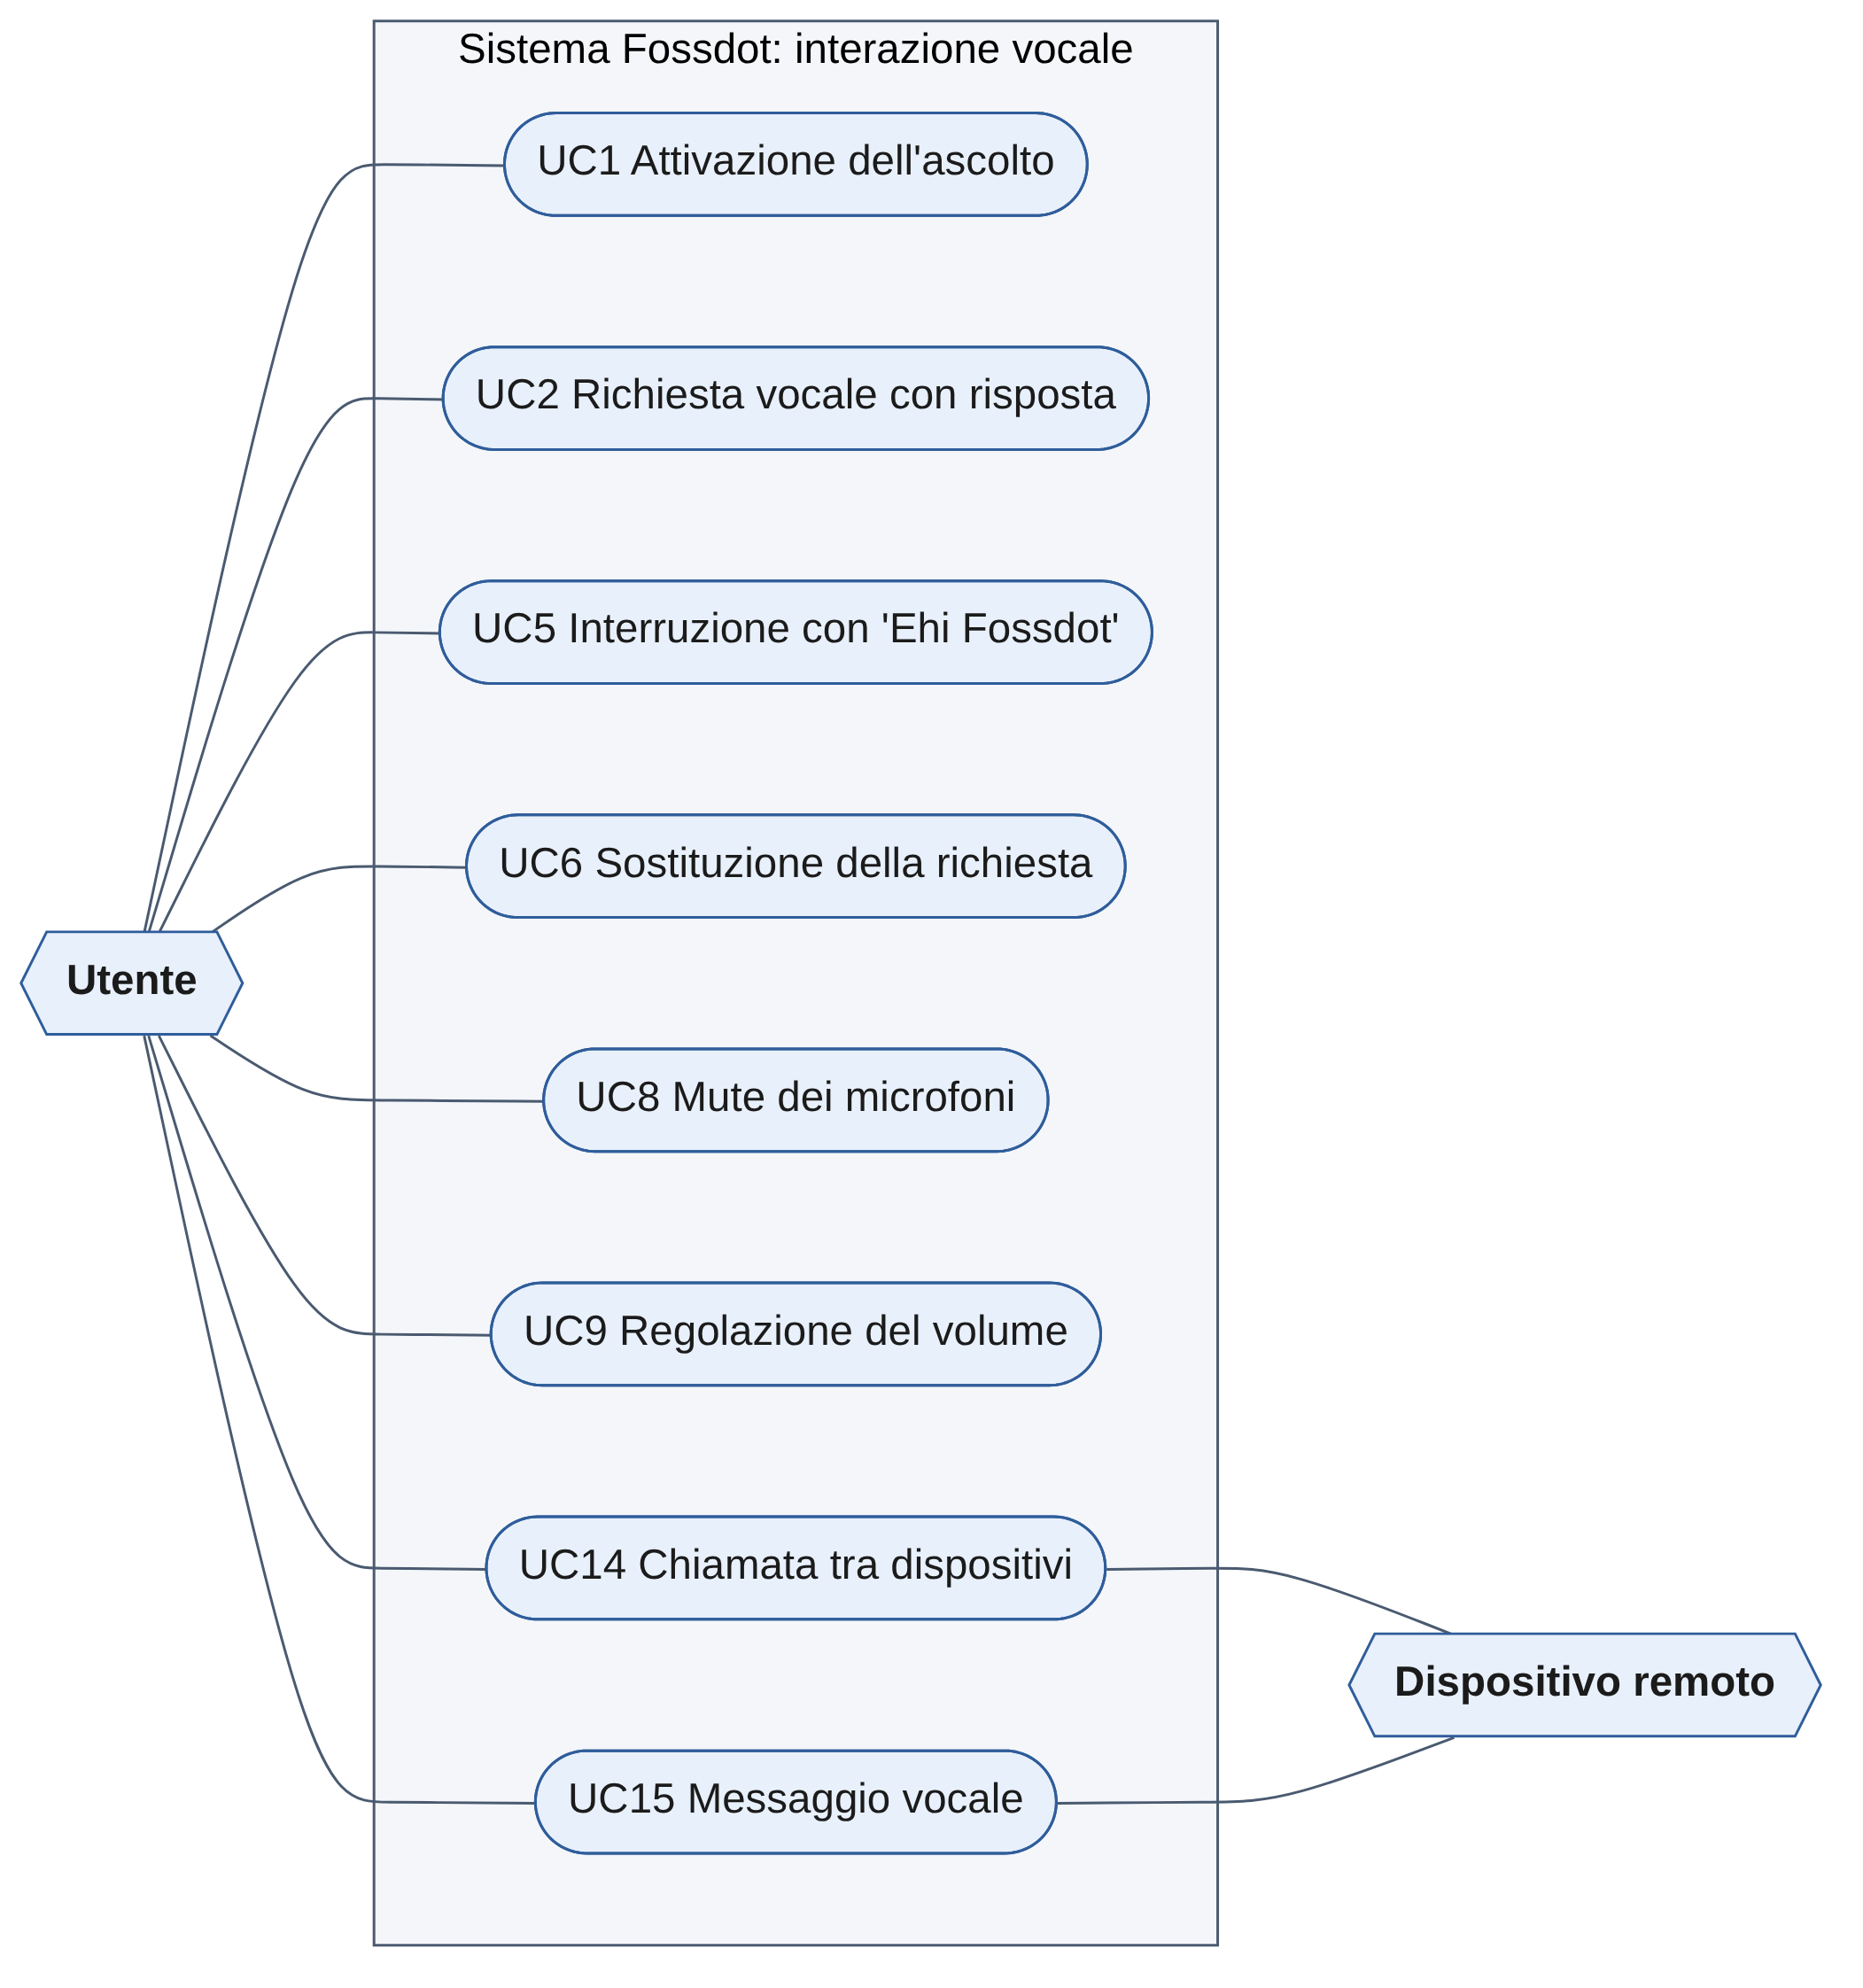
\includegraphics[width=\linewidth,height=0.62\textheight,keepaspectratio]{img_adr/10-uc-vocali.png}
\caption{Casi d'uso dell'interazione vocale (UC1, UC2, UC5, UC6, UC8, UC9, UC14, UC15)}
\end{figure}

\begin{figure}[H]
\centering
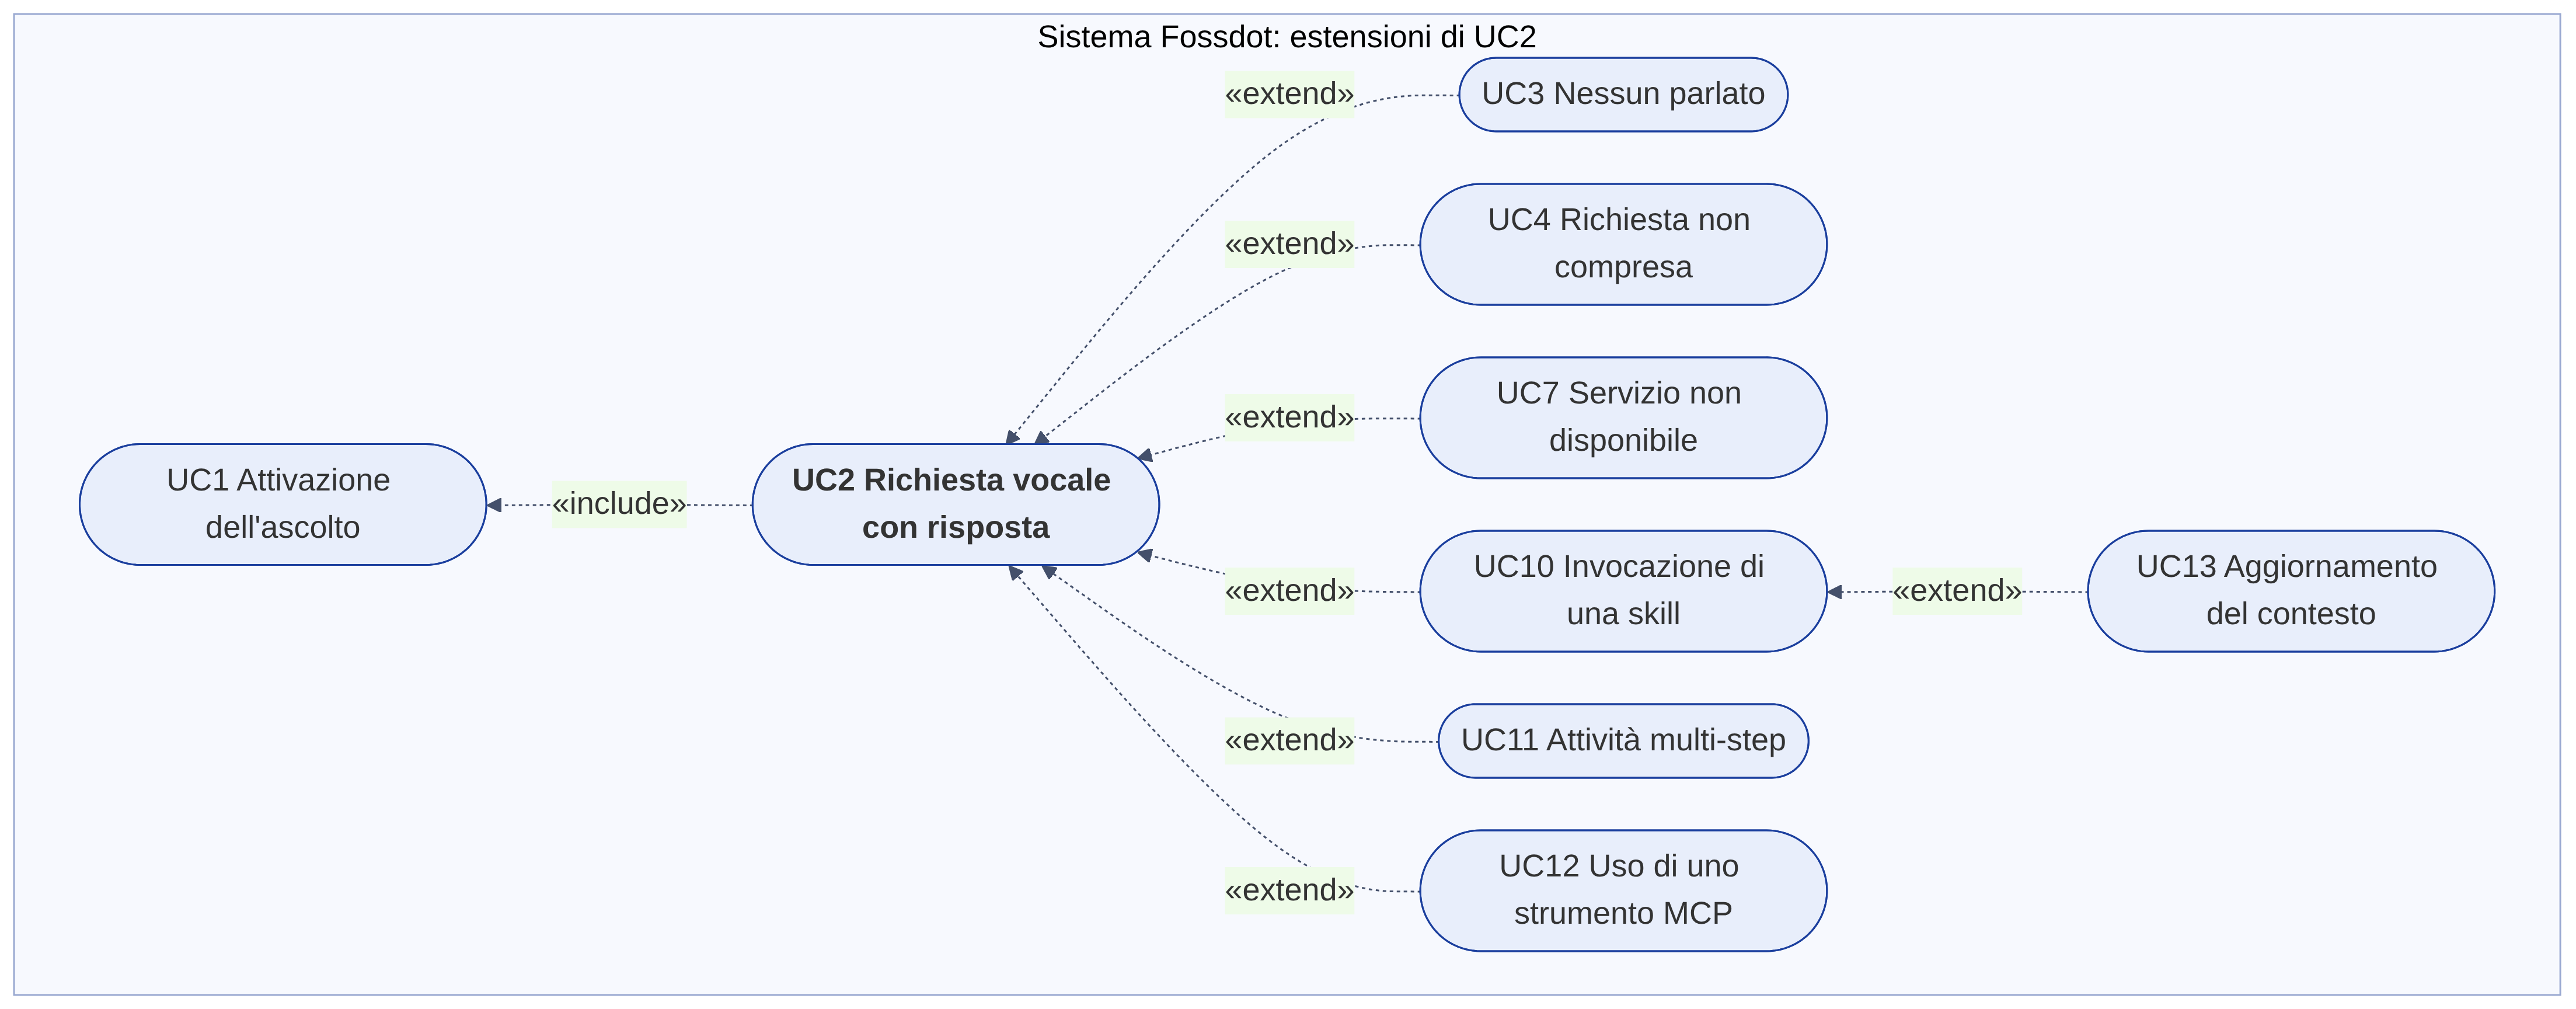
\includegraphics[width=\linewidth,height=0.62\textheight,keepaspectratio]{img_adr/10b-uc-richiesta.png}
\caption{Inclusioni ed estensioni della richiesta vocale (UC2, UC3, UC4, UC7, UC10--UC13)}
\end{figure}

\subsubsection{UC1 -- Attivazione dell'ascolto}

\begin{itemize}
\tightlist
\item \textbf{Attore primario:} Utente.
\item \textbf{Precondizioni:} il dispositivo è nello stato \emph{Inattivo} (ST-4), connesso al server, con i microfoni attivi.
\item \textbf{Postcondizioni:} il dispositivo è nello stato \emph{In ascolto} (ST-5) e sul server è aperta una sessione vocale per quel dispositivo.
\item \textbf{Scenario principale:}
\begin{enumerate}
\tightlist
\item L'Utente pronuncia la \emph{wake word} oppure preme il pulsante azione.
\item Il dispositivo riconosce l'attivazione in locale, senza inviare audio all'esterno.
\item Il dispositivo emette un suono breve e mostra lo stato ``in ascolto'' sui LED.
\item Il dispositivo apre una sessione vocale sul server.
\end{enumerate}
\item \textbf{Generalizzazioni:} UC1 è specializzato da UC1.1 e UC1.2, che differiscono solo per il modo di attivazione (passo 1).
\item \textbf{Fonte:} Capitolato, VE 21/10.
\end{itemize}

\paragraph{UC1.1 -- Attivazione con wake word}
\begin{itemize}
\tightlist
\item \textbf{Attore primario:} Utente.
\item \textbf{Differenza rispetto a UC1:} al passo 1 l'Utente pronuncia la \emph{wake word}; il riconoscimento avviene sempre sul dispositivo (RV-3).
\item \textbf{Fonte:} Capitolato, VE 21/10.
\end{itemize}

\paragraph{UC1.2 -- Attivazione con pulsante (push-to-talk)}
\begin{itemize}
\tightlist
\item \textbf{Attore primario:} Utente.
\item \textbf{Differenza rispetto a UC1:} al passo 1 l'Utente preme il pulsante azione.
\item \textbf{Fonte:} Capitolato (``\emph{wake word} o \emph{push-to-talk}'').
\end{itemize}

\subsubsection{UC2 -- Richiesta vocale con risposta}

\begin{itemize}
\tightlist
\item \textbf{Attore primario:} Utente. \textbf{Servizi coinvolti:} \emph{provider} AI, trascrizione (STT), sintesi vocale (TTS).
\item \textbf{Precondizioni:} il dispositivo è \emph{Inattivo} (ST-4) e connesso; per il dispositivo è configurato un \emph{provider} AI.
\item \textbf{Postcondizioni:} la risposta è stata riprodotta; il dispositivo è \emph{Inattivo} (ST-4).
\item \textbf{Scenario principale:}
\begin{enumerate}
\tightlist
\item L'Utente attiva l'ascolto (UC1).
\item L'Utente pronuncia la richiesta; il dispositivo la invia al server in \emph{streaming} (UC2.1).
\item Il server rileva la fine della richiesta e il dispositivo passa allo stato \emph{Elaborazione} (ST-6).
\item Il server trascrive l'audio.
\item Il server invia la trascrizione al \emph{provider} AI configurato per il dispositivo, con il contesto e gli strumenti disponibili.
\item Il server converte la risposta in audio e la invia al dispositivo in \emph{streaming} (UC2.2).
\item Il dispositivo riproduce la risposta nello stato \emph{Risposta} (ST-7), poi torna \emph{Inattivo}.
\end{enumerate}
\item \textbf{Inclusioni:} UC1 (passo 1), UC2.1 (passo 2), UC2.2 (passo 6).
\item \textbf{Estensioni:}
\begin{itemize}
\tightlist
\item al passo 2, nessun parlato entro il tempo di attesa: UC3;
\item al passo 4, trascrizione vuota o non riconoscibile: UC4;
\item ai passi 4--6, servizio non raggiungibile o in errore: UC7;
\item al passo 5, il modello sceglie lo strumento di una \emph{skill}: UC10; più strumenti in sequenza: UC11; uno strumento MCP: UC12.
\end{itemize}
\item \textbf{Fonte:} Capitolato (MVP: dimostrazione ``\emph{wake word} \textrightarrow{} domanda \textrightarrow{} risposta vocale'').
\end{itemize}

\paragraph{UC2.1 -- Acquisizione della richiesta e rilevamento della fine}
\begin{itemize}
\tightlist
\item \textbf{Attore primario:} Utente.
\item \textbf{Precondizioni:} il dispositivo è \emph{In ascolto} (ST-5).
\item \textbf{Postcondizioni:} il server ha ricevuto l'audio completo della richiesta; il dispositivo è in \emph{Elaborazione} (ST-6).
\item \textbf{Scenario principale:}
\begin{enumerate}
\tightlist
\item Mentre l'Utente parla, il dispositivo invia frame audio di durata fissa (RP-7).
\item Il server considera conclusa la richiesta dopo un silenzio continuo (RP-4) o al raggiungimento della durata massima (RP-6).
\item Il server comunica al dispositivo la fine dell'ascolto.
\end{enumerate}
\item \textbf{Fonte:} Capitolato, Interna.
\end{itemize}

\paragraph{UC2.2 -- Ricezione della risposta vocale}
\begin{itemize}
\tightlist
\item \textbf{Attore primario:} Utente.
\item \textbf{Precondizioni:} il modello sta producendo la risposta; il dispositivo è in \emph{Elaborazione} (ST-6).
\item \textbf{Postcondizioni:} l'audio della risposta è stato riprodotto per intero; il server ha inviato il messaggio di fine risposta.
\item \textbf{Scenario principale:}
\begin{enumerate}
\tightlist
\item Il server converte la risposta in audio per frasi, appena il modello le produce.
\item Il server invia l'audio a blocchi; il dispositivo passa a \emph{Risposta} (ST-7) e inizia a riprodurlo prima che la risposta sia completa.
\item Al termine il server invia un messaggio di fine risposta.
\end{enumerate}
\item \textbf{Fonte:} Interna.
\end{itemize}

\subsubsection{UC3 -- Nessun parlato dopo l'attivazione}
\begin{itemize}
\tightlist
\item \textbf{Attore primario:} Utente.
\item \textbf{Precondizioni:} il dispositivo è \emph{In ascolto} (ST-5) e non ha ricevuto parlato.
\item \textbf{Postcondizioni:} la sessione vocale è chiusa senza contattare il \emph{provider} AI; il dispositivo è \emph{Inattivo} (ST-4).
\item \textbf{Scenario principale:}
\begin{enumerate}
\tightlist
\item Trascorre il tempo di attesa (RP-5) senza parlato.
\item Il server chiude la sessione.
\item Il dispositivo dà un riscontro discreto e torna \emph{Inattivo}.
\end{enumerate}
\item \textbf{Estende:} UC2, al passo 2.
\item \textbf{Fonte:} Interna.
\end{itemize}

\subsubsection{UC4 -- Richiesta non compresa}
\begin{itemize}
\tightlist
\item \textbf{Attore primario:} Utente.
\item \textbf{Precondizioni:} il dispositivo è in \emph{Elaborazione} (ST-6); la trascrizione della richiesta è vuota o non contiene parlato riconoscibile.
\item \textbf{Postcondizioni:} il \emph{provider} AI non è stato contattato; il dispositivo è \emph{Inattivo} (ST-4).
\item \textbf{Scenario principale:}
\begin{enumerate}
\tightlist
\item Il server rileva che la trascrizione non è utilizzabile.
\item Il dispositivo riproduce un messaggio come ``Scusa, non ho capito''.
\item Il dispositivo torna \emph{Inattivo}.
\end{enumerate}
\item \textbf{Estende:} UC2, al passo 4.
\item \textbf{Fonte:} Interna.
\end{itemize}

\subsubsection{UC5 -- Interruzione della risposta con ``Ehi Fossdot''}

\begin{figure}[H]
\centering
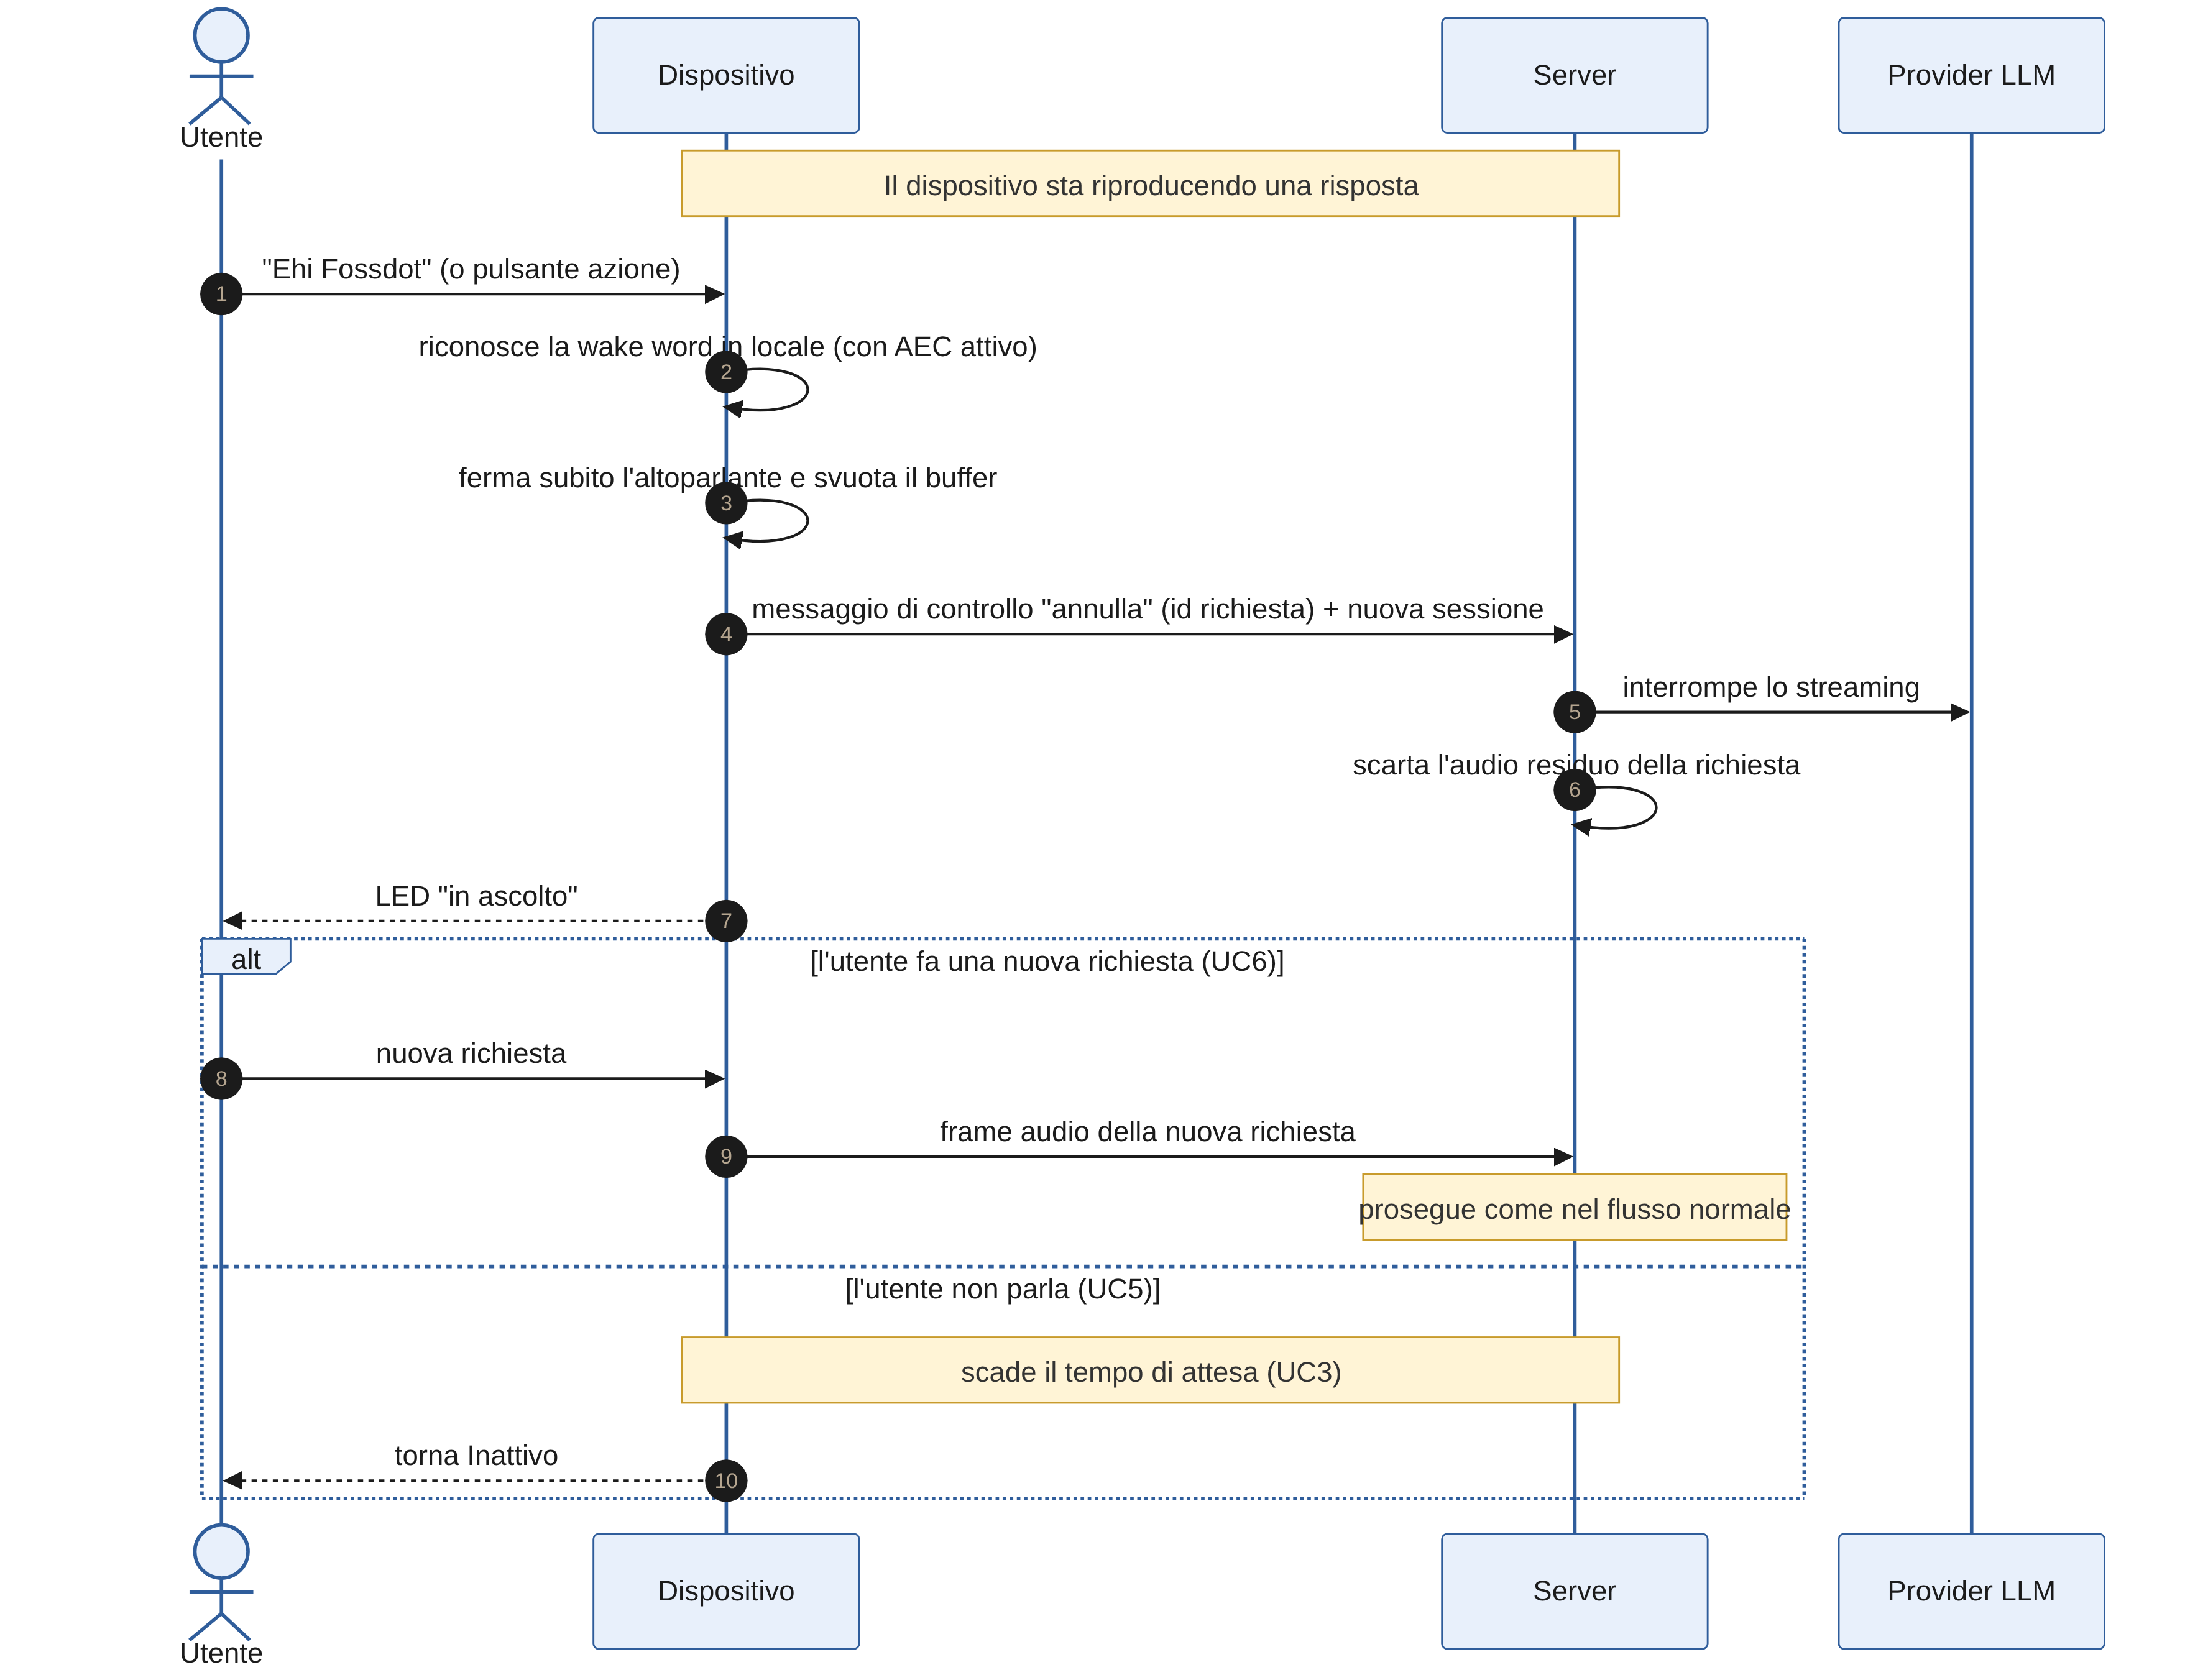
\includegraphics[width=\linewidth,height=0.62\textheight,keepaspectratio]{img_adr/06-sequenza-interruzione.png}
\caption{Sequenza dell'interruzione della risposta (UC5, UC6)}
\end{figure}

\begin{itemize}
\tightlist
\item \textbf{Attore primario:} Utente.
\item \textbf{Precondizioni:} il dispositivo è nello stato \emph{Risposta} (ST-7).
\item \textbf{Postcondizioni:} la riproduzione è ferma; la richiesta è annullata sul server; il dispositivo è \emph{In ascolto} (ST-5).
\item \textbf{Scenario principale:}
\begin{enumerate}
\tightlist
\item L'Utente pronuncia la \emph{wake word} (``Ehi Fossdot'').
\item Il dispositivo la riconosce in locale e ferma subito l'altoparlante (RP-3).
\item Il dispositivo invia al server un messaggio di annullamento.
\item Il server interrompe la generazione del modello e la sintesi e scarta l'audio residuo.
\item Il dispositivo passa a \emph{In ascolto}: se l'Utente non parla, torna \emph{Inattivo} (UC3); se fa una nuova richiesta, il caso prosegue come UC6.
\end{enumerate}
\item \textbf{Scenario alternativo:} al passo 1 l'Utente preme il pulsante azione; il resto non cambia.
\item \textbf{Note:} non esiste una parola ``stop'' separata: l'interruzione usa lo stesso meccanismo di UC6.
\item \textbf{Fonte:} VE 13/11 (soluzione proposta dal gruppo e approvata da Uranion), Interna.
\end{itemize}

\subsubsection{UC6 -- Sostituzione della richiesta in corso}
\begin{itemize}
\tightlist
\item \textbf{Attore primario:} Utente.
\item \textbf{Precondizioni:} il dispositivo è in \emph{Elaborazione} (ST-6) o in \emph{Risposta} (ST-7).
\item \textbf{Postcondizioni:} la richiesta precedente è annullata sul server; il dispositivo è \emph{In ascolto} (ST-5) per la nuova richiesta.
\item \textbf{Scenario principale:}
\begin{enumerate}
\tightlist
\item L'Utente pronuncia di nuovo la \emph{wake word}.
\item Il dispositivo ferma la riproduzione e invia l'annullamento al server.
\item Il server annulla la richiesta in corso.
\item Il dispositivo passa a \emph{In ascolto} e la nuova richiesta prosegue come in UC2 dal passo 2.
\end{enumerate}
\item \textbf{Fonte:} VE 13/11.
\end{itemize}

\subsubsection{UC7 -- Servizio non disponibile}
\begin{itemize}
\tightlist
\item \textbf{Attore primario:} Utente. \textbf{Servizi coinvolti:} \emph{provider} AI, STT, TTS.
\item \textbf{Precondizioni:} è in corso una richiesta (UC2); il server non è raggiungibile, oppure \emph{provider}, STT o TTS restituiscono un errore o superano il tempo massimo (RP-12).
\item \textbf{Postcondizioni:} la richiesta è chiusa senza risposta; l'errore è registrato nei log del server; il dispositivo è \emph{Inattivo} (ST-4) o \emph{Non connesso} (ST-11).
\item \textbf{Scenario principale:}
\begin{enumerate}
\tightlist
\item Il server rileva l'errore o lo scadere del tempo massimo.
\item Il server chiude la richiesta e invia al dispositivo un messaggio vocale di errore.
\item Il dispositivo mostra lo stato \emph{Errore} (ST-10), riproduce il messaggio e torna \emph{Inattivo}.
\end{enumerate}
\item \textbf{Scenario alternativo:} il server non è raggiungibile; il dispositivo riproduce un suono memorizzato localmente e passa a \emph{Non connesso}.
\item \textbf{Estende:} UC2, ai passi 4--6.
\item \textbf{Fonte:} Interna, Capitolato (affidabilità del flusso \emph{end-to-end}).
\end{itemize}

\subsubsection{UC8 -- Mute dei microfoni}
\begin{itemize}
\tightlist
\item \textbf{Attore primario:} Utente.
\item \textbf{Precondizioni:} il dispositivo è \emph{Inattivo} (ST-4).
\item \textbf{Postcondizioni:} il dispositivo è \emph{Muto} (ST-8): non acquisisce audio, nemmeno per la \emph{wake word}.
\item \textbf{Scenario principale:}
\begin{enumerate}
\tightlist
\item L'Utente aziona il comando di mute.
\item Il dispositivo smette di acquisire audio e mostra un LED fisso dedicato.
\end{enumerate}
\item \textbf{Scenario alternativo:} con il dispositivo \emph{Muto}, l'Utente aziona di nuovo il comando; i microfoni si riattivano e il dispositivo torna \emph{Inattivo}.
\item \textbf{Fonte:} Interna, coerente con la privacy richiesta dal Capitolato.
\end{itemize}

\subsubsection{UC9 -- Regolazione del volume}
\begin{itemize}
\tightlist
\item \textbf{Attore primario:} Utente.
\item \textbf{Precondizioni:} il dispositivo è acceso e connesso.
\item \textbf{Postcondizioni:} il nuovo livello di volume è applicato e memorizzato sul dispositivo.
\item \textbf{Scenario principale:}
\begin{enumerate}
\tightlist
\item L'Utente chiede di alzare o abbassare il volume.
\item Il dispositivo applica il nuovo livello e lo mostra sui LED.
\end{enumerate}
\item \textbf{Generalizzazioni:} UC9 è specializzato da UC9.1 e UC9.2, che differiscono solo per il modo in cui l'Utente dà il comando (passo 1).
\item \textbf{Fonte:} Interna.
\end{itemize}

\paragraph{UC9.1 -- Impostazione del volume con i tasti}
\begin{itemize}
\tightlist
\item \textbf{Attore primario:} Utente.
\item \textbf{Differenza rispetto a UC9:} al passo 1 l'Utente alza o abbassa il volume con i tasti del dispositivo.
\item \textbf{Fonte:} Interna.
\end{itemize}

\paragraph{UC9.2 -- Impostazione del volume a voce}
\begin{itemize}
\tightlist
\item \textbf{Attore primario:} Utente.
\item \textbf{Differenza rispetto a UC9:} al passo 1 l'Utente chiede a voce di alzare o abbassare il volume; la richiesta segue il flusso di UC2.
\item \textbf{Fonte:} Interna.
\end{itemize}

\subsubsection{UC10 -- Invocazione di una skill}
\begin{itemize}
\tightlist
\item \textbf{Attore primario:} Utente.
\item \textbf{Precondizioni:} almeno una \emph{skill} è installata e abilitata per il dispositivo; il dispositivo è in \emph{Elaborazione} (ST-6).
\item \textbf{Postcondizioni:} la \emph{skill} è stata eseguita e il suo risultato è stato usato per la risposta.
\item \textbf{Scenario principale:}
\begin{enumerate}
\tightlist
\item L'Utente fa una richiesta che corrisponde a una \emph{skill} (ad esempio ``che tempo fa domani?'').
\item Il modello sceglie lo strumento della \emph{skill} e ne indica gli argomenti.
\item Il server esegue la \emph{skill} e restituisce il risultato al modello.
\item Il modello formula la risposta, che prosegue come in UC2 dal passo 6.
\end{enumerate}
\item \textbf{Estende:} UC2, al passo 5.
\item \textbf{Estensioni:} al passo 3, la \emph{skill} fallisce: UC10.1; al passo 2, mancano parametri: UC10.2; al passo 3, lo strumento è segnato come da confermare: UC10.3; la \emph{skill} è quella di sistema per il contesto: UC13.
\item \textbf{Fonte:} Capitolato (versione completa), VE 21/10 (almeno una \emph{skill} dimostrativa).
\end{itemize}

\paragraph{UC10.1 -- Errore nell'esecuzione di una skill}
\begin{itemize}
\tightlist
\item \textbf{Attore primario:} Utente.
\item \textbf{Precondizioni:} l'esecuzione della \emph{skill} è terminata con un errore o ha superato il tempo massimo.
\item \textbf{Postcondizioni:} la richiesta è chiusa; il dispositivo è \emph{Inattivo} (ST-4).
\item \textbf{Scenario principale:} il server comunica l'errore al modello, che formula un messaggio comprensibile; il dispositivo lo riproduce e torna \emph{Inattivo}.
\item \textbf{Estende:} UC10, al passo 3.
\item \textbf{Fonte:} Interna.
\end{itemize}

\paragraph{UC10.2 -- Richiesta di un dato mancante}
\begin{itemize}
\tightlist
\item \textbf{Attore primario:} Utente.
\item \textbf{Precondizioni:} la \emph{skill} richiede un parametro che la richiesta non contiene.
\item \textbf{Postcondizioni:} la \emph{skill} è eseguita con il dato fornito, oppure la richiesta è chiusa se l'Utente non risponde.
\item \textbf{Scenario principale:} il dispositivo chiede a voce il dato mancante; l'Utente risponde senza ripetere la \emph{wake word}; lo scenario riprende da UC10 al passo 3.
\item \textbf{Estende:} UC10, al passo 2.
\item \textbf{Fonte:} Interna.
\end{itemize}

\paragraph{UC10.3 -- Conferma di un'azione con effetti esterni}
\begin{itemize}
\tightlist
\item \textbf{Attore primario:} Utente.
\item \textbf{Precondizioni:} lo strumento scelto dal modello è segnato come da confermare (ad esempio invio di un messaggio, modifica del calendario, cancellazione di dati).
\item \textbf{Postcondizioni:} lo strumento è stato eseguito solo se l'Utente ha confermato; altrimenti l'azione è annullata e nulla è cambiato.
\item \textbf{Scenario principale:}
\begin{enumerate}
\tightlist
\item Il server sospende l'esecuzione dello strumento.
\item Il dispositivo descrive a voce l'azione e i suoi dati e chiede conferma (ad esempio ``Mando a Luca: arrivo tra dieci minuti. Confermi?'').
\item L'Utente risponde ``sì'' senza ripetere la \emph{wake word}.
\item Lo scenario riprende da UC10 al passo 3.
\end{enumerate}
\item \textbf{Scenario alternativo:} al passo 3 l'Utente risponde ``no'' o non risponde entro il tempo previsto; il server annulla l'azione e il dispositivo lo comunica a voce.
\item \textbf{Estende:} UC10, al passo 3 (vale anche per gli strumenti MCP di UC12).
\item \textbf{Fonte:} Interna.
\end{itemize}

\subsubsection{UC11 -- Attività multi-step (agent)}

\begin{figure}[H]
\centering
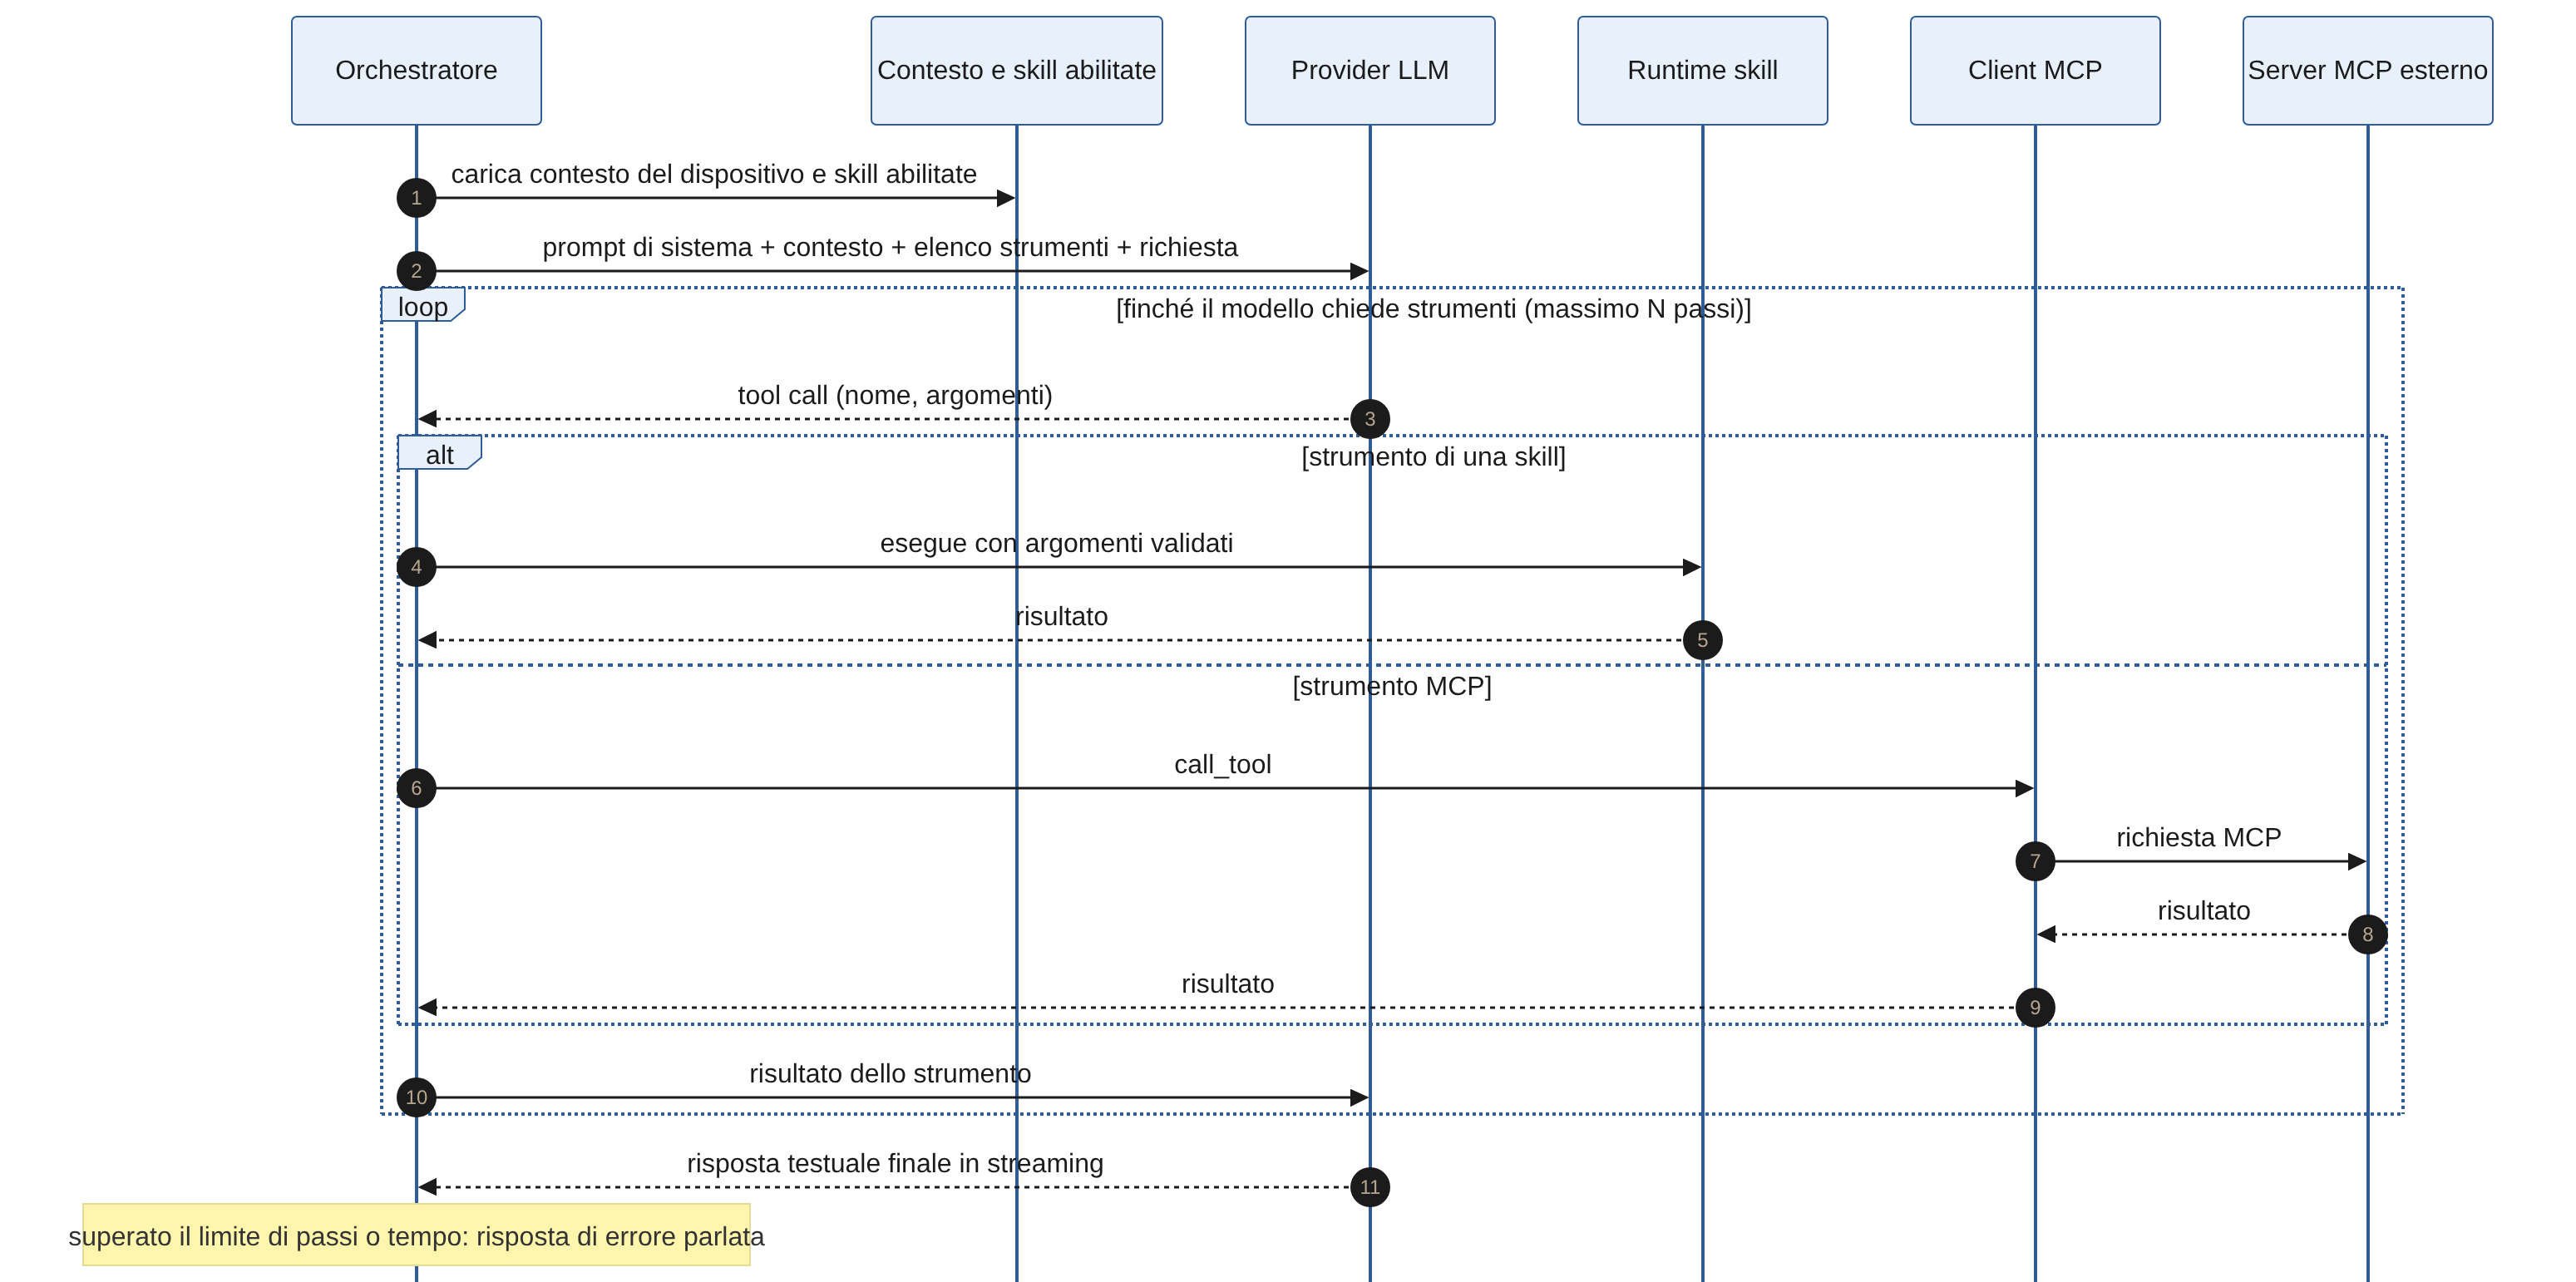
\includegraphics[width=\linewidth,height=0.62\textheight,keepaspectratio]{img_adr/08-sequenza-strumenti.png}
\caption{Ciclo delle chiamate agli strumenti (UC10, UC11, UC12)}
\end{figure}

\begin{itemize}
\tightlist
\item \textbf{Attore primario:} Utente.
\item \textbf{Precondizioni:} il dispositivo è in \emph{Elaborazione} (ST-6); sono disponibili più strumenti (\emph{skill} o MCP).
\item \textbf{Postcondizioni:} l'attività è completata entro il numero massimo di passi e il tempo massimo, oppure è chiusa con un messaggio di errore.
\item \textbf{Scenario principale:}
\begin{enumerate}
\tightlist
\item L'Utente chiede un'attività che richiede più passi (ad esempio ``cerca la ricetta della carbonara e mandala alla cucina'').
\item Il modello chiama uno strumento e il server gli restituisce il risultato.
\item Il passo 2 si ripete finché il modello non ha la risposta.
\item La risposta prosegue come in UC2 dal passo 6.
\end{enumerate}
\item \textbf{Scenario alternativo:} al passo 3 si raggiunge il numero massimo di passi o il tempo massimo; il server chiude l'attività e il dispositivo riproduce un messaggio di errore.
\item \textbf{Estende:} UC2, al passo 5.
\item \textbf{Fonte:} Capitolato (Agents attivabili a voce).
\end{itemize}

\subsubsection{UC12 -- Uso di uno strumento MCP}
\begin{itemize}
\tightlist
\item \textbf{Attore primario:} Utente. \textbf{Servizi coinvolti:} server MCP.
\item \textbf{Precondizioni:} almeno un server MCP è configurato, raggiungibile e con strumenti abilitati; il dispositivo è in \emph{Elaborazione} (ST-6).
\item \textbf{Postcondizioni:} lo strumento MCP è stato eseguito e il suo risultato è stato usato per la risposta.
\item \textbf{Scenario principale:} come UC10, ma al passo 3 il server Fossdot, in qualità di client MCP, invoca lo strumento sul server MCP.
\item \textbf{Scenario alternativo:} il server MCP non risponde; si procede come in UC10.1.
\item \textbf{Estende:} UC2, al passo 5.
\item \textbf{Fonte:} Capitolato.
\end{itemize}

\subsubsection{UC13 -- Aggiornamento del contesto a voce}
\begin{itemize}
\tightlist
\item \textbf{Attore primario:} Utente.
\item \textbf{Precondizioni:} la \emph{skill} di sistema per il contesto è abilitata per il dispositivo.
\item \textbf{Postcondizioni:} al testo di contesto del dispositivo è aggiunta una nuova informazione, usata dalle richieste successive; le parti già presenti non sono cambiate.
\item \textbf{Scenario principale:}
\begin{enumerate}
\tightlist
\item L'Utente dice ad esempio ``ricorda che sono un ingegnere del \emph{software}, rispondimi in modo tecnico''.
\item Il modello invoca la \emph{skill} di sistema per il contesto.
\item Il server aggiunge l'informazione in fondo al testo di contesto del dispositivo e il dispositivo conferma a voce.
\end{enumerate}
\item \textbf{Scenario alternativo:} al passo 1 l'Utente chiede di dimenticare o cambiare un'informazione già presente; il dispositivo risponde che può farlo solo l'Amministratore dalla web app (UC36).
\item \textbf{Estende:} UC10, al passo 2.
\item \textbf{Fonte:} VE 13/11 (indicata da Uranion come \emph{skill} interessante).
\end{itemize}

\subsubsection{UC14 -- Chiamata tra dispositivi}

\begin{figure}[H]
\centering
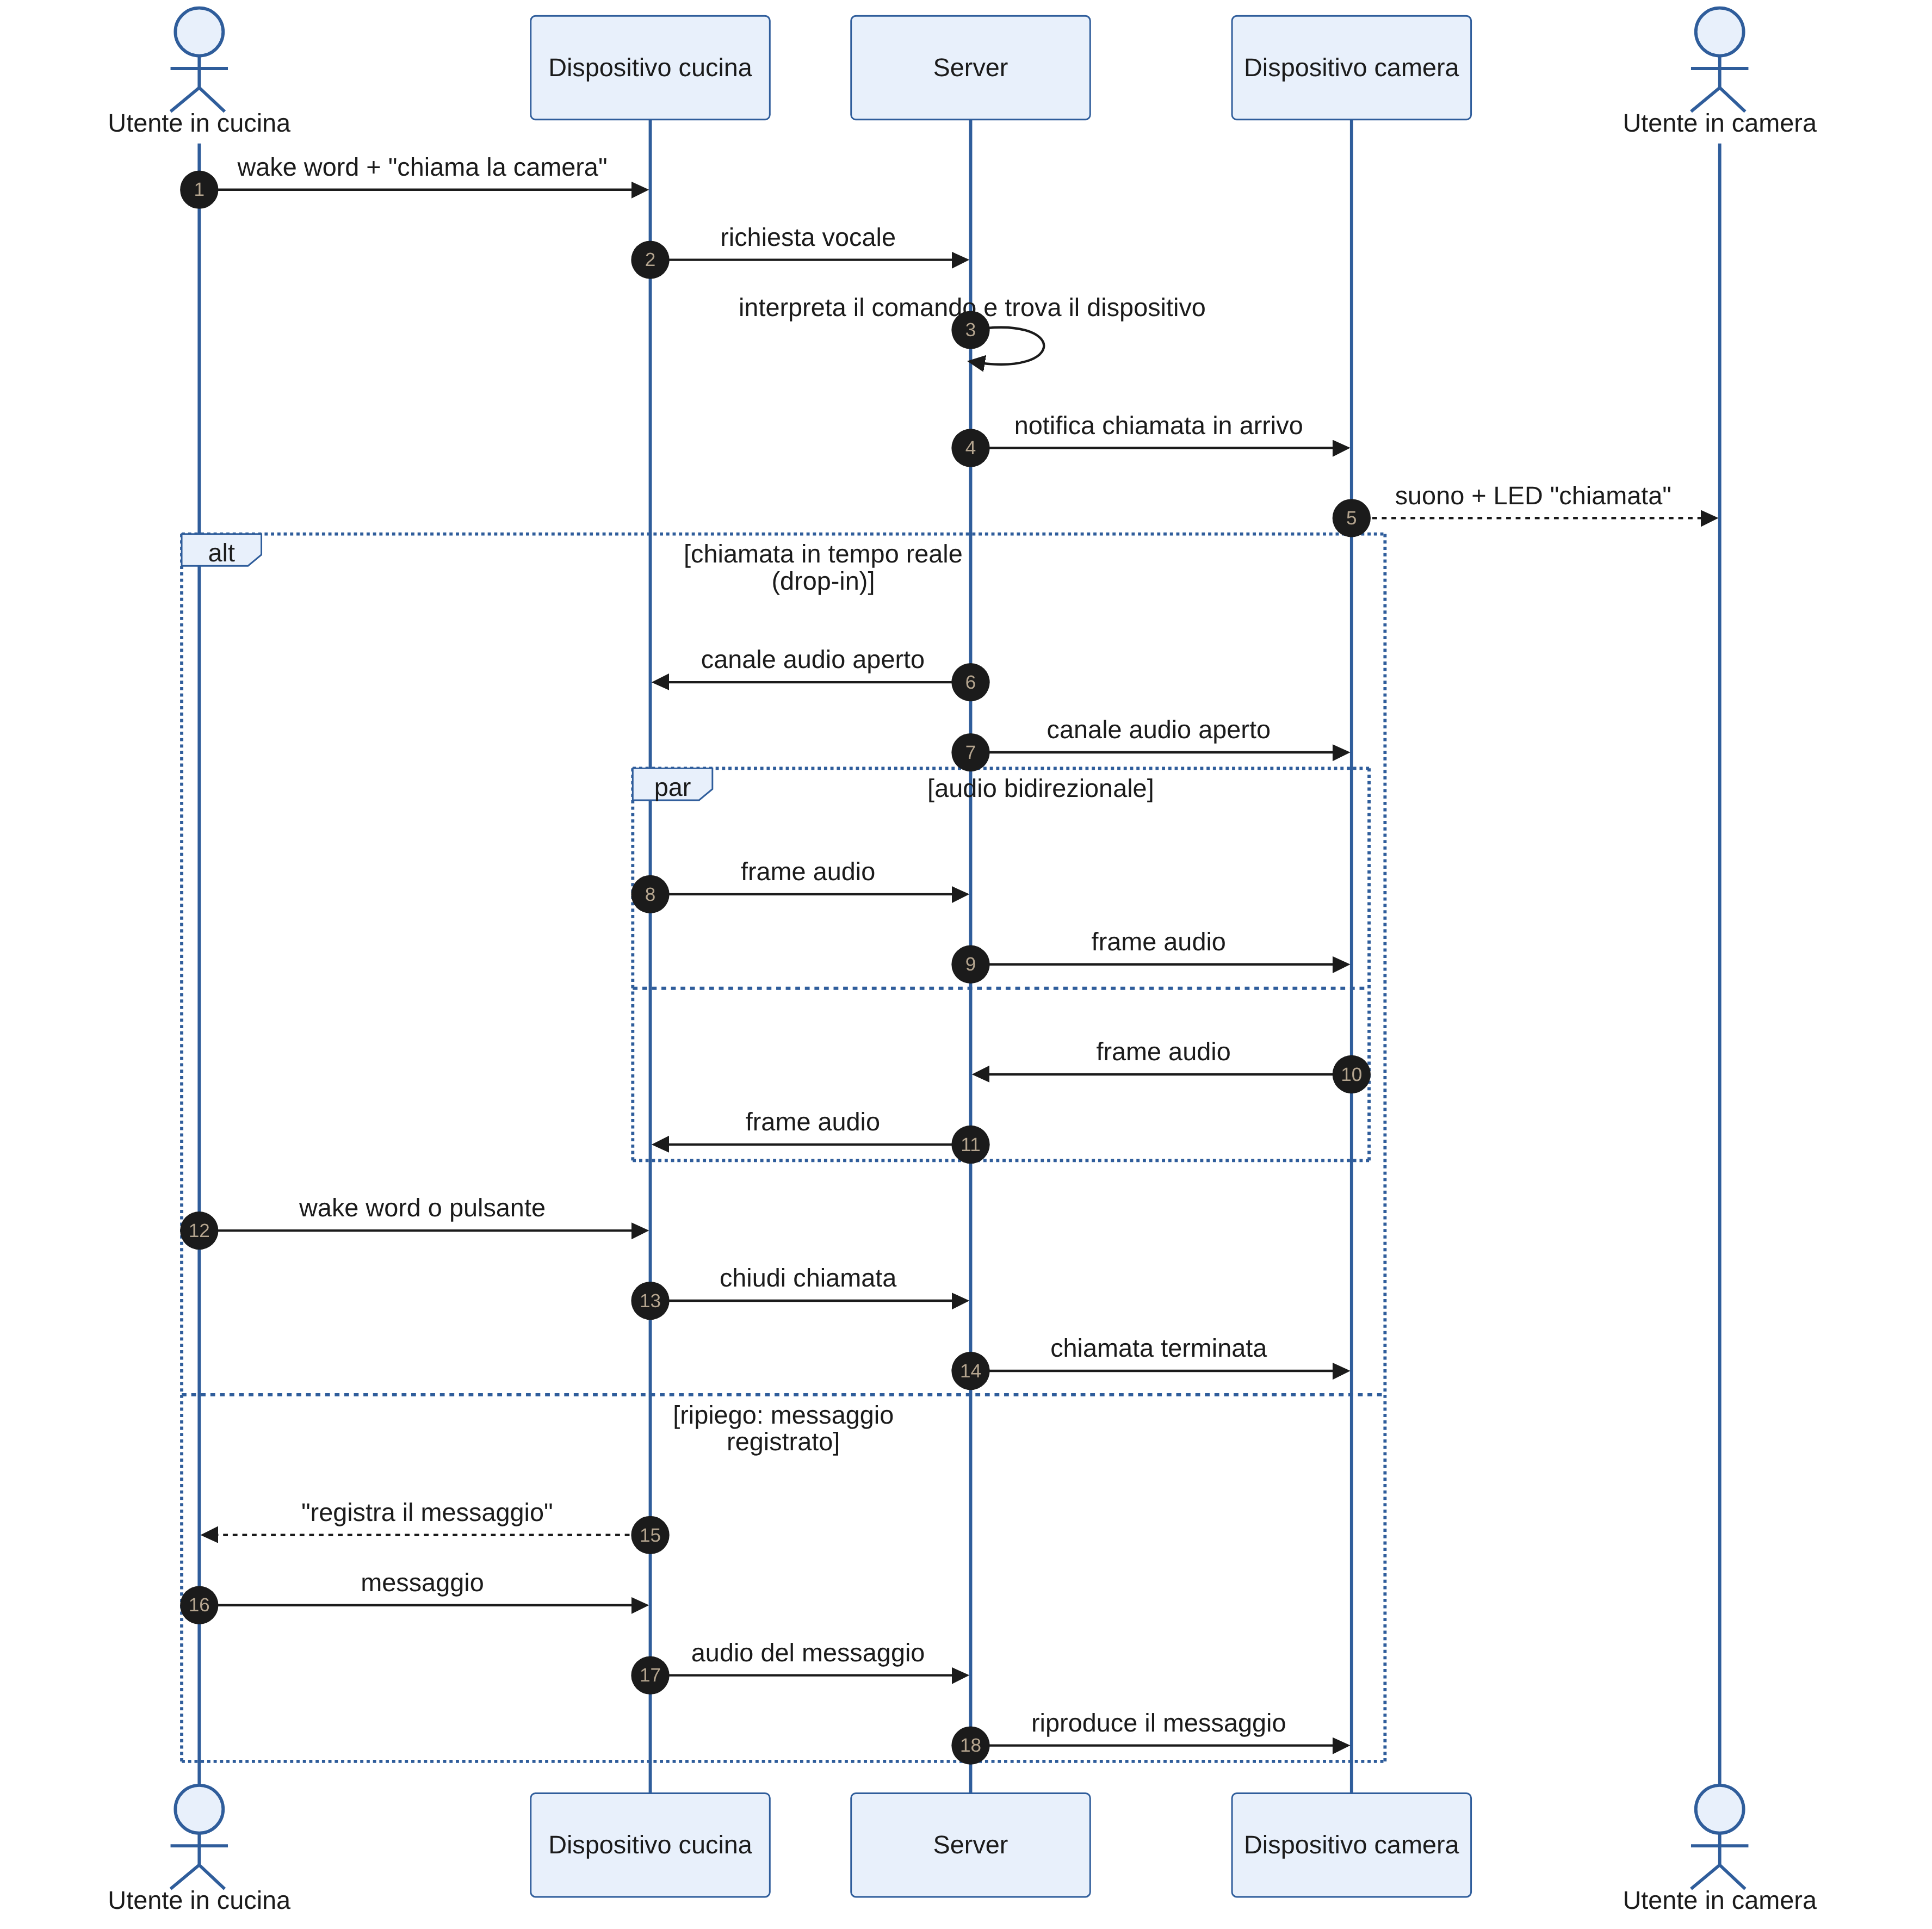
\includegraphics[width=\linewidth,height=0.62\textheight,keepaspectratio]{img_adr/09-sequenza-chiamata.png}
\caption{Sequenza di una chiamata tra dispositivi (UC14)}
\end{figure}

\begin{itemize}
\tightlist
\item \textbf{Attore primario:} Utente. \textbf{Attore secondario:} Dispositivo remoto.
\item \textbf{Precondizioni:} almeno due dispositivi sono associati alla stessa casa e connessi; il dispositivo chiamante è \emph{Inattivo} (ST-4).
\item \textbf{Postcondizioni:} la chiamata è terminata e i due dispositivi sono \emph{Inattivi}.
\item \textbf{Scenario principale:}
\begin{enumerate}
\tightlist
\item L'Utente avvia la chiamata (UC14.1).
\item Il dispositivo remoto riceve la chiamata (UC14.2).
\item I due dispositivi scambiano audio in tempo reale nello stato \emph{Chiamata} (ST-9).
\item Uno dei due Utenti termina la chiamata (UC14.3).
\end{enumerate}
\item \textbf{Inclusioni:} UC14.1, UC14.2, UC14.3.
\item \textbf{Estensioni:} al passo 1, il dispositivo richiesto non esiste o non è connesso: UC14.4.
\item \textbf{Fonte:} VE 21/10 (funzione \emph{drop in}, obiettivo del progetto), Capitolato (intercom).
\end{itemize}

\paragraph{UC14.1 -- Avvio di una chiamata}
\begin{itemize}
\tightlist
\item \textbf{Attore primario:} Utente.
\item \textbf{Scenario principale:} l'Utente dice ad esempio ``chiama la camera''; il server individua il dispositivo dal nome o dalla stanza e apre un canale audio bidirezionale in tempo reale.
\item \textbf{Fonte:} VE 21/10.
\end{itemize}

\paragraph{UC14.2 -- Ricezione di una chiamata}
\begin{itemize}
\tightlist
\item \textbf{Attore primario:} Utente. \textbf{Attore secondario:} Dispositivo remoto.
\item \textbf{Scenario principale:} il dispositivo remoto emette un suono e mostra lo stato \emph{Chiamata} sui LED; l'audio passa subito nei due sensi (\emph{drop in}).
\item \textbf{Fonte:} VE 21/10.
\end{itemize}

\paragraph{UC14.3 -- Termine della chiamata}
\begin{itemize}
\tightlist
\item \textbf{Attore primario:} Utente.
\item \textbf{Scenario principale:} uno dei due Utenti pronuncia la \emph{wake word} o preme il pulsante azione; entrambi i dispositivi chiudono il canale e tornano \emph{Inattivi}.
\item \textbf{Fonte:} Interna.
\end{itemize}

\paragraph{UC14.4 -- Dispositivo da chiamare non disponibile}
\begin{itemize}
\tightlist
\item \textbf{Attore primario:} Utente.
\item \textbf{Precondizioni:} il nome o la stanza indicati non corrispondono a un dispositivo connesso della casa.
\item \textbf{Postcondizioni:} nessun canale audio è aperto; il dispositivo chiamante è \emph{Inattivo} (ST-4).
\item \textbf{Scenario principale:} il server non trova il dispositivo; il dispositivo chiamante riproduce un messaggio vocale di errore.
\item \textbf{Estende:} UC14, al passo 1.
\item \textbf{Fonte:} Interna.
\end{itemize}

\subsubsection{UC15 -- Messaggio vocale verso un altro dispositivo}
\begin{itemize}
\tightlist
\item \textbf{Attore primario:} Utente. \textbf{Attore secondario:} Dispositivo remoto.
\item \textbf{Precondizioni:} almeno due dispositivi sono associati alla stessa casa.
\item \textbf{Postcondizioni:} il messaggio è stato riprodotto sul dispositivo destinatario, oppure è in attesa sul server finché il destinatario non si connette.
\item \textbf{Scenario principale:}
\begin{enumerate}
\tightlist
\item L'Utente chiede di inviare un messaggio a un altro dispositivo e lo registra.
\item Il server consegna il messaggio al dispositivo destinatario.
\item Il dispositivo destinatario lo riproduce appena è \emph{Inattivo}.
\end{enumerate}
\item \textbf{Fonte:} VE 21/10 (soluzione di ripiego se la chiamata in tempo reale è troppo complessa).
\end{itemize}

\subsection{Dispositivo}

\begin{figure}[H]
\centering
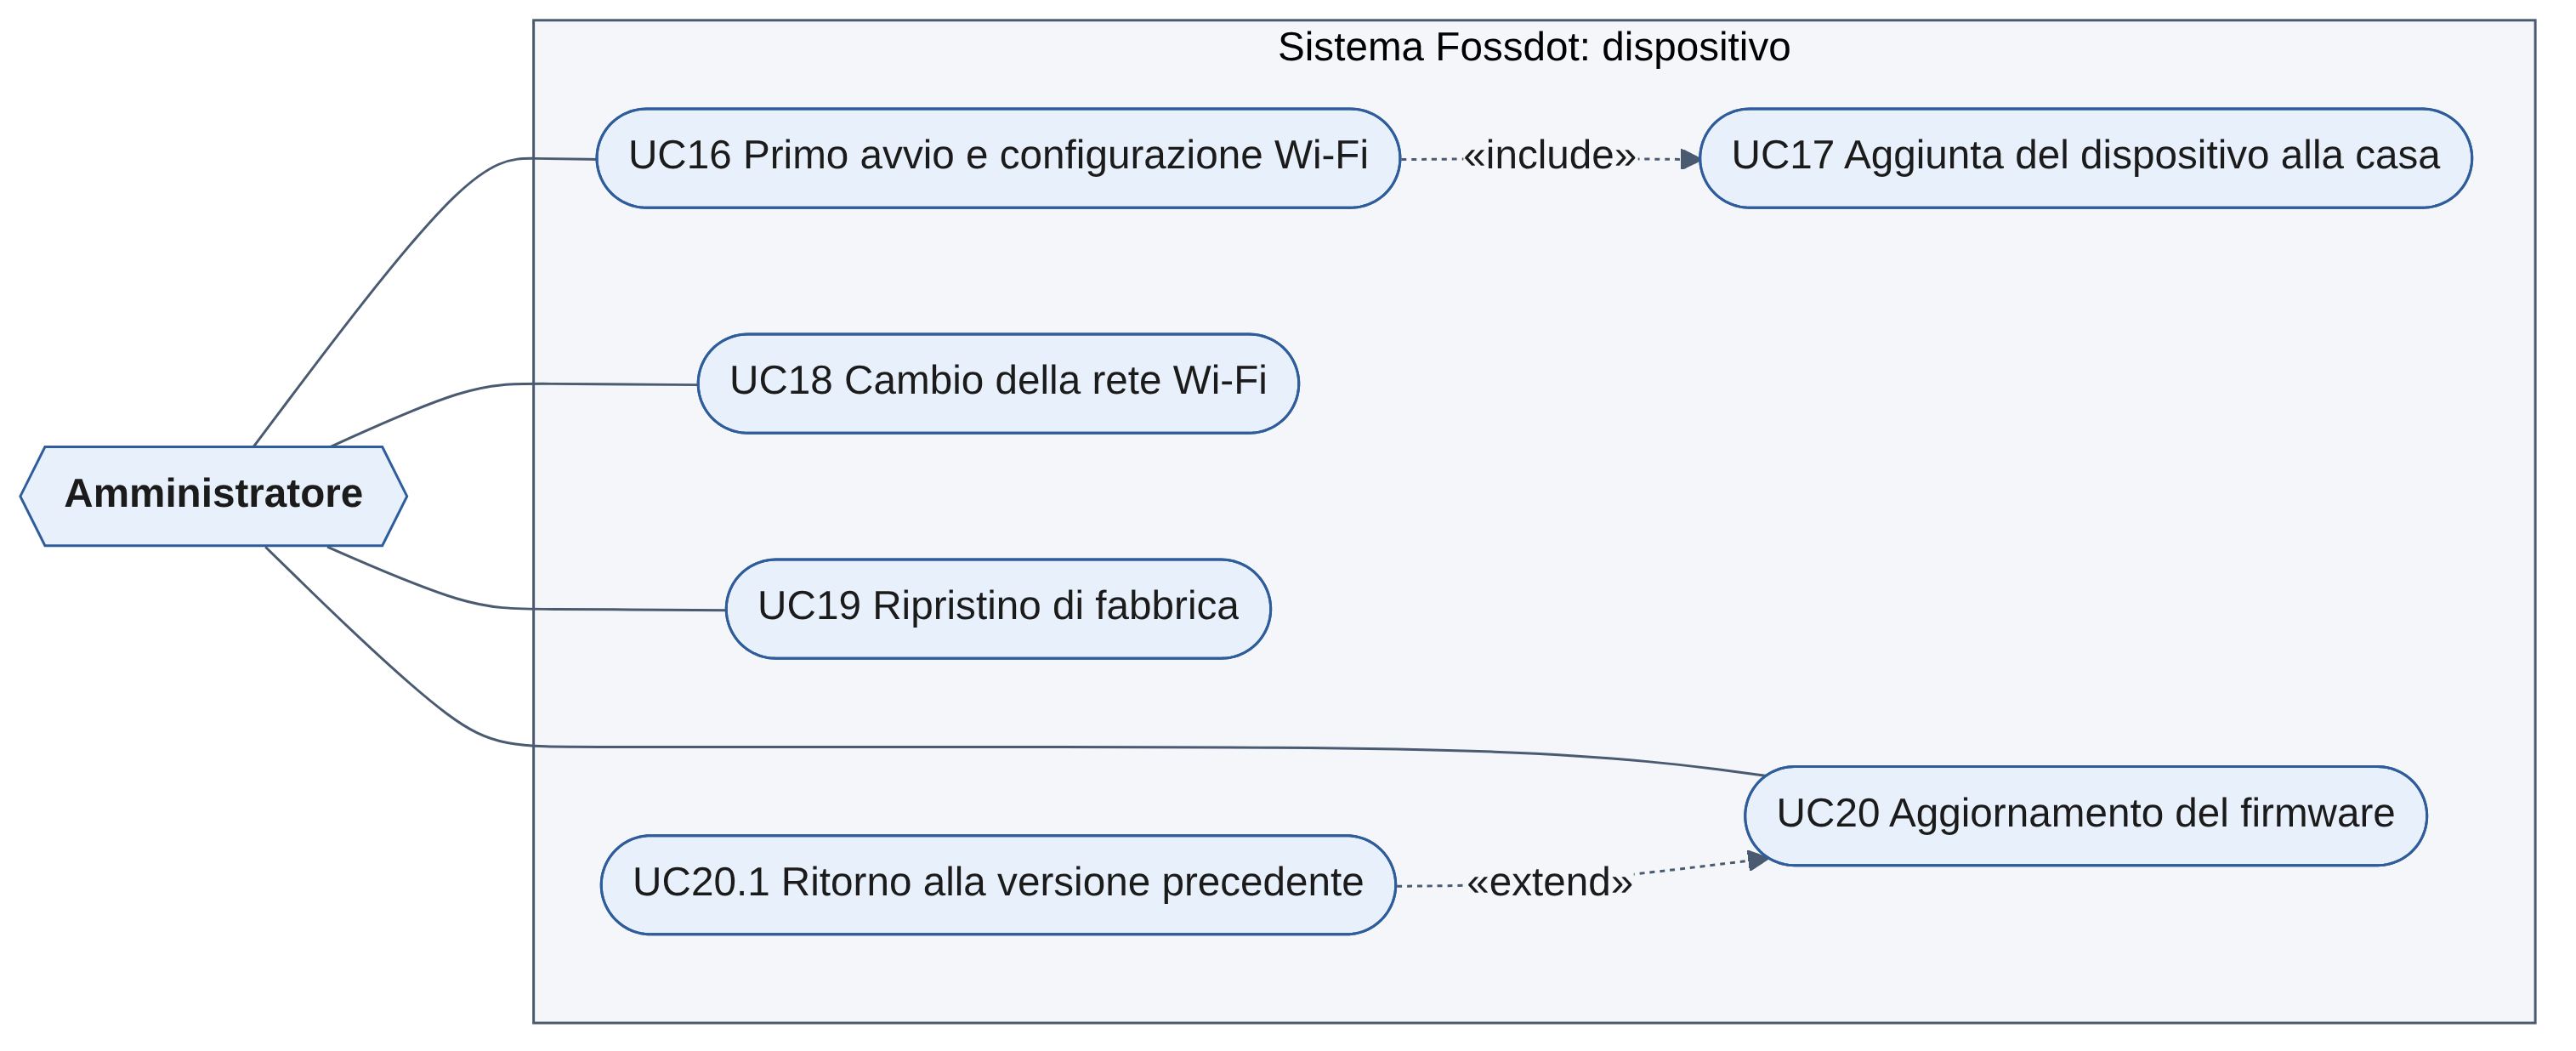
\includegraphics[width=\linewidth,height=0.62\textheight,keepaspectratio]{img_adr/11-uc-dispositivo.png}
\caption{Casi d'uso del dispositivo (UC16--UC20)}
\end{figure}

\begin{figure}[H]
\centering
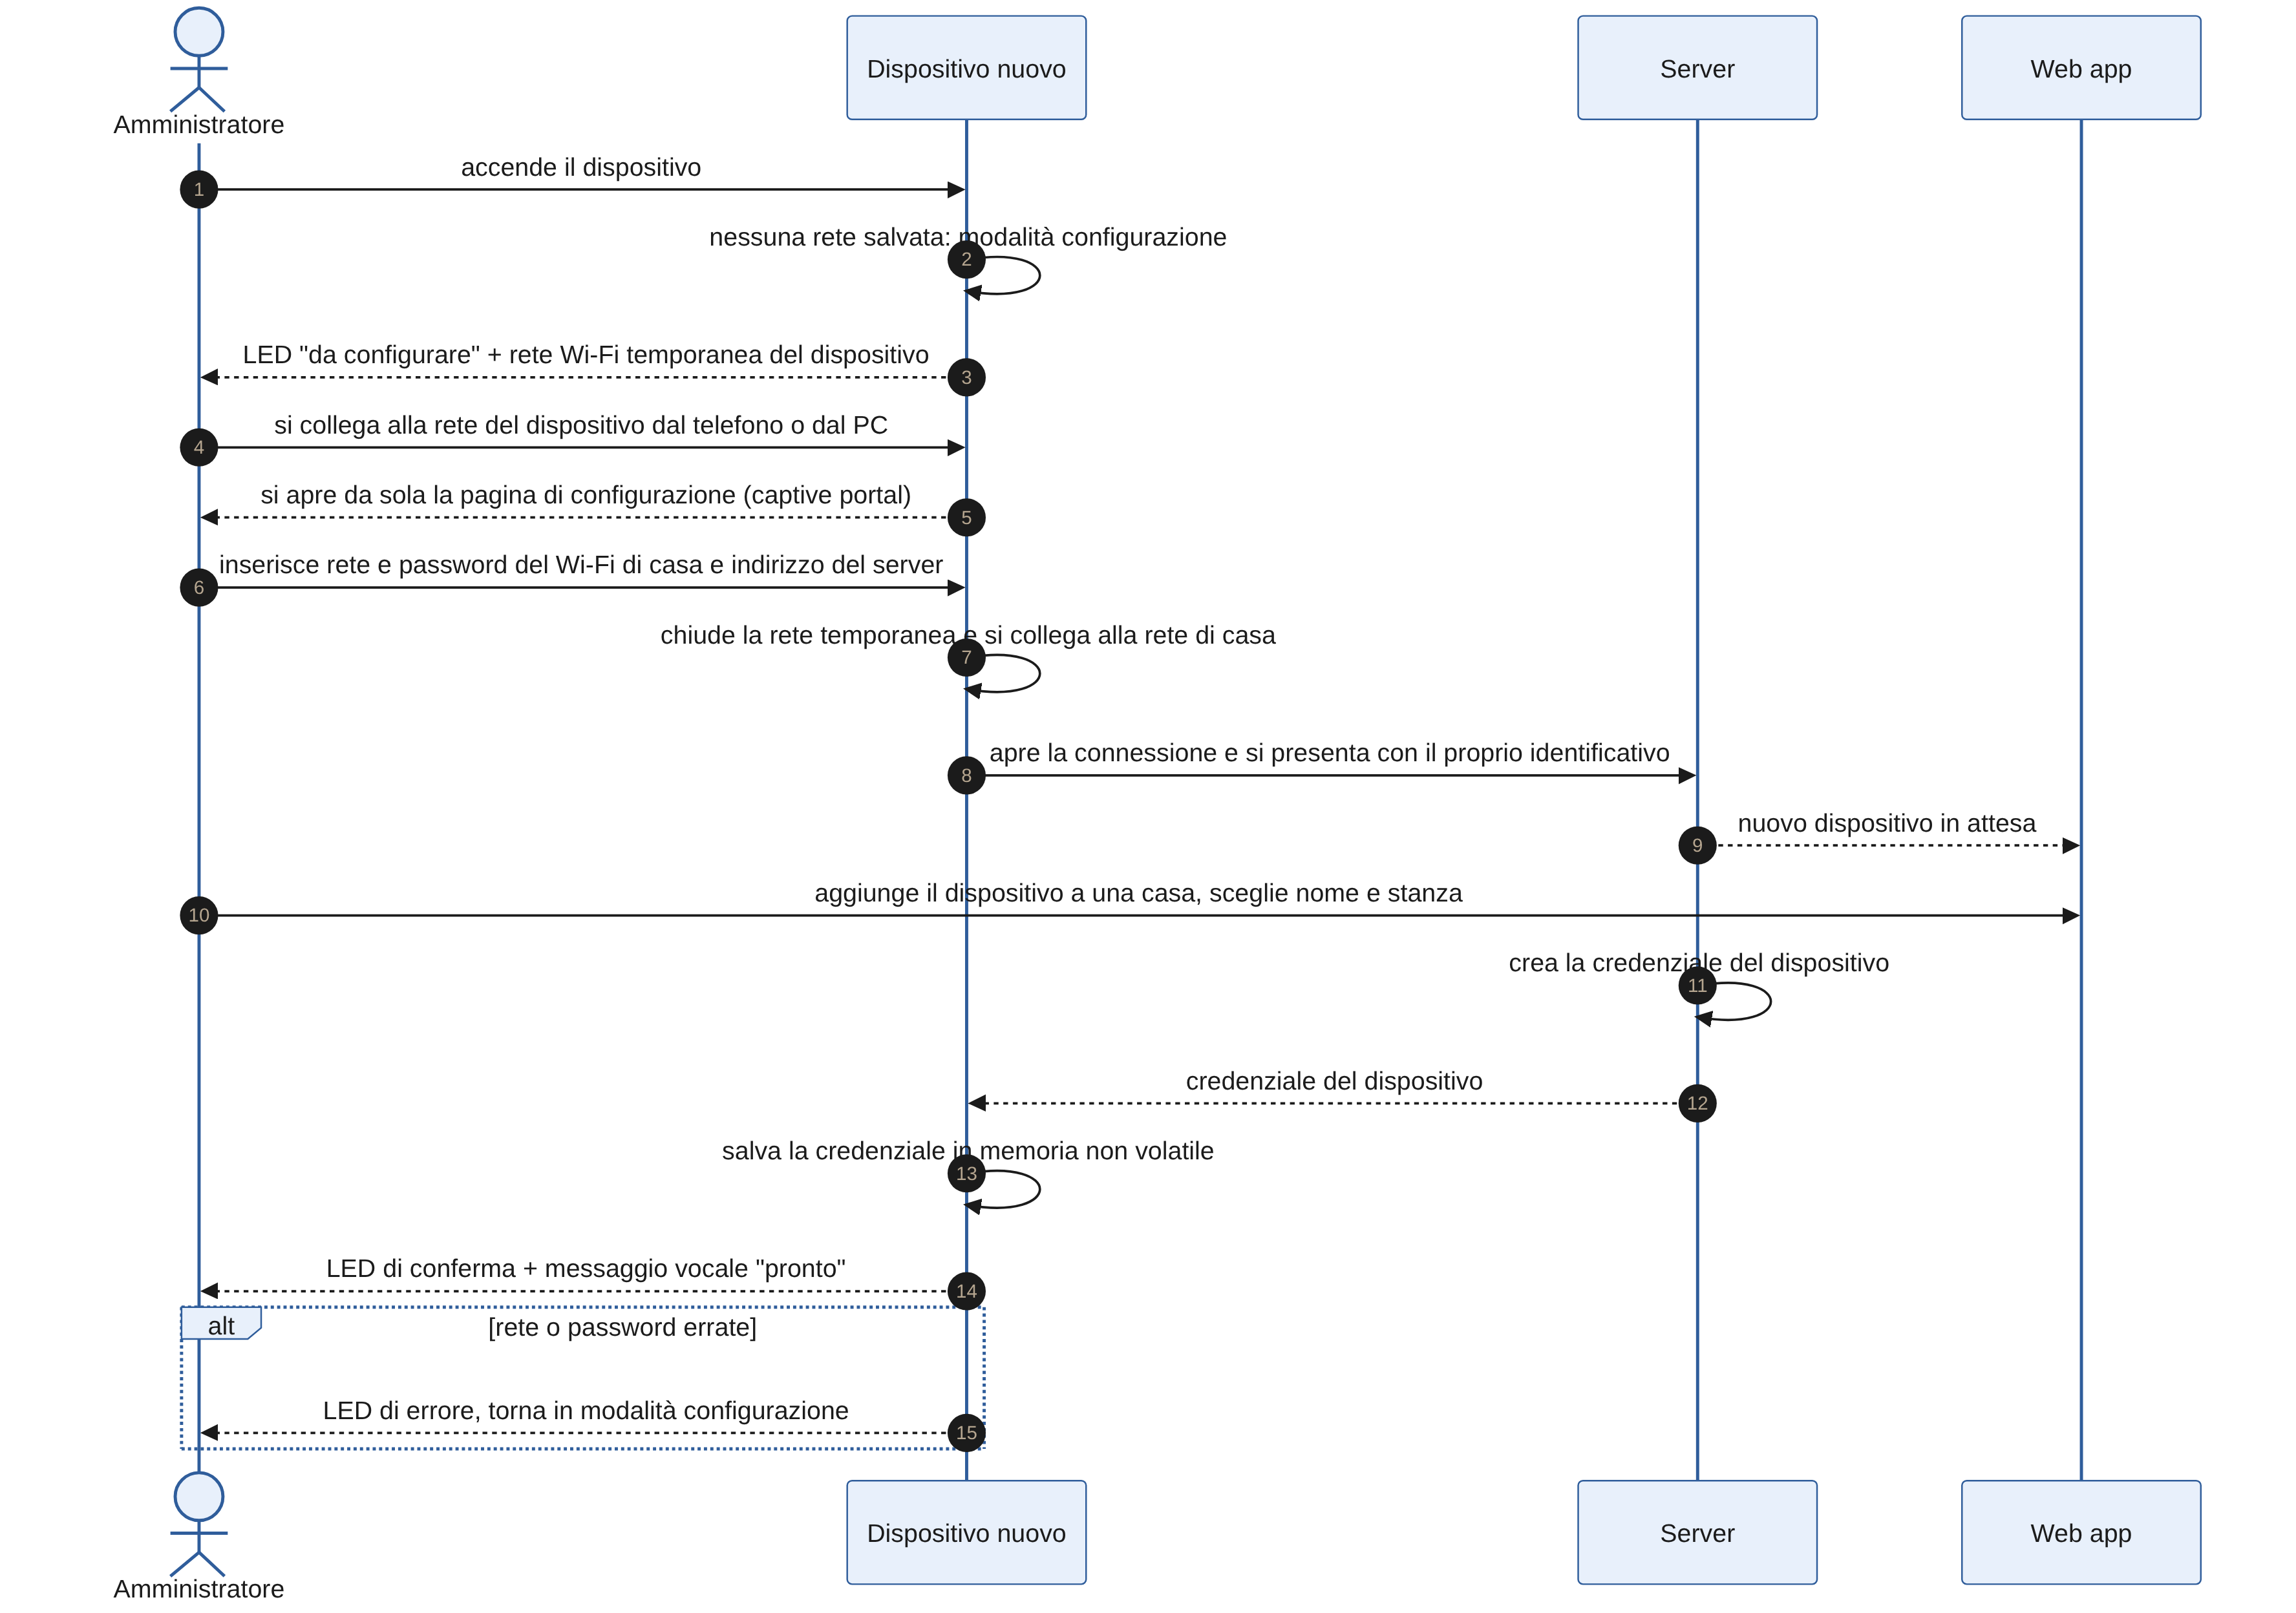
\includegraphics[width=\linewidth,height=0.62\textheight,keepaspectratio]{img_adr/07-sequenza-onboarding.png}
\caption{Sequenza dell'\emph{onboarding} del dispositivo (UC16, UC17)}
\end{figure}

\subsubsection{UC16 -- Primo avvio e configurazione del Wi-Fi}
\begin{itemize}
\tightlist
\item \textbf{Attore primario:} Amministratore.
\item \textbf{Precondizioni:} il dispositivo non ha una rete salvata (nuovo o ripristinato) ed è nello stato \emph{Onboarding} (ST-2); l'Amministratore ha un account.
\item \textbf{Postcondizioni:} il dispositivo ha una rete salvata, è connesso al server ed è associato alla casa dell'Amministratore.
\item \textbf{Scenario principale:}
\begin{enumerate}
\tightlist
\item L'Amministratore accende il dispositivo, che segnala con i LED lo stato \emph{Onboarding}.
\item Il dispositivo crea una propria rete Wi-Fi temporanea.
\item L'Amministratore si collega a questa rete dal telefono o dal PC; la pagina di configurazione si apre da sola (\emph{captive portal}), senza installare \emph{software}.
\item L'Amministratore inserisce rete e password del Wi-Fi di casa e l'indirizzo del server.
\item Il dispositivo chiude la rete temporanea, si collega alla rete di casa e al server.
\item L'Amministratore aggiunge il dispositivo a una casa dalla web app (UC17).
\item Il dispositivo conferma con LED e messaggio vocale e passa a \emph{Inattivo}.
\end{enumerate}
\item \textbf{Inclusioni:} UC17 (passo 6).
\item \textbf{Estensioni:} al passo 5, rete o password errate: UC16.1.
\item \textbf{Fonte:} Capitolato (registrazione del dispositivo), VE 21/10 (\emph{onboarding} molto curato).
\end{itemize}

\paragraph{UC16.1 -- Rete o password errate}
\begin{itemize}
\tightlist
\item \textbf{Attore primario:} Amministratore.
\item \textbf{Precondizioni:} il dispositivo non riesce a collegarsi alla rete indicata.
\item \textbf{Postcondizioni:} il dispositivo è di nuovo in \emph{Onboarding} (ST-2), con la pagina di configurazione disponibile.
\item \textbf{Scenario principale:} il dispositivo mostra l'errore con i LED e torna al passo 2 di UC16.
\item \textbf{Estende:} UC16, al passo 5.
\item \textbf{Fonte:} VE 21/10.
\end{itemize}

\subsubsection{UC17 -- Aggiunta del dispositivo alla casa}
\begin{itemize}
\tightlist
\item \textbf{Attore primario:} Amministratore.
\item \textbf{Precondizioni:} l'Amministratore è autenticato nella web app; il dispositivo è connesso al server (ST-3) ma non appartiene ancora a nessuna casa.
\item \textbf{Postcondizioni:} il dispositivo appartiene alla casa, ha una credenziale propria e compare nell'elenco dei dispositivi.
\item \textbf{Scenario principale:}
\begin{enumerate}
\tightlist
\item Il dispositivo si presenta al server con il proprio identificativo.
\item La web app mostra all'Amministratore il nuovo dispositivo in attesa di essere aggiunto.
\item L'Amministratore lo aggiunge a una delle sue case e ne sceglie nome e stanza.
\item Il server assegna al dispositivo una credenziale propria, che il dispositivo conserva e usa a ogni connessione.
\end{enumerate}
\item \textbf{Scenario alternativo:} al passo 3 l'Amministratore rifiuta il dispositivo, che resta senza casa e non può usare il server.
\item \textbf{Fonte:} Capitolato (registrazione e autenticazione del dispositivo), VE 21/10.
\end{itemize}

\subsubsection{UC18 -- Cambio della rete Wi-Fi}
\begin{itemize}
\tightlist
\item \textbf{Attore primario:} Amministratore.
\item \textbf{Precondizioni:} il dispositivo è associato a una casa.
\item \textbf{Postcondizioni:} il dispositivo è connesso alla nuova rete e resta associato alla stessa casa.
\item \textbf{Scenario principale:}
\begin{enumerate}
\tightlist
\item L'Amministratore riporta il dispositivo in \emph{Onboarding} con un comando fisico.
\item L'Amministratore inserisce la nuova rete e la password dalla pagina di configurazione.
\item Il dispositivo si collega alla nuova rete e al server senza ripetere l'associazione.
\end{enumerate}
\item \textbf{Estensioni:} al passo 3, rete o password errate: come UC16.1.
\item \textbf{Fonte:} Interna.
\end{itemize}

\subsubsection{UC19 -- Ripristino di fabbrica}
\begin{itemize}
\tightlist
\item \textbf{Attore primario:} Amministratore.
\item \textbf{Precondizioni:} il dispositivo è acceso.
\item \textbf{Postcondizioni:} sul dispositivo non restano rete, credenziali né configurazione; il dispositivo è in \emph{Onboarding} (ST-2).
\item \textbf{Scenario principale:}
\begin{enumerate}
\tightlist
\item L'Amministratore esegue la combinazione di comandi fisici prevista per il ripristino.
\item Il dispositivo cancella rete, credenziali e configurazione e si riavvia.
\item Al primo tentativo di accesso fallito il server segna il dispositivo come dissociato.
\end{enumerate}
\item \textbf{Scenario alternativo:} al passo 3 l'Amministratore rimuove il dispositivo dalla web app (UC30.5).
\item \textbf{Fonte:} Interna.
\end{itemize}

\subsubsection{UC20 -- Aggiornamento del firmware}
\begin{itemize}
\tightlist
\item \textbf{Attore primario:} Amministratore. \textbf{Servizi coinvolti:} servizio di aggiornamento del \emph{firmware}.
\item \textbf{Precondizioni:} è disponibile una versione del \emph{firmware} più recente di quella installata; il dispositivo è \emph{Inattivo} (ST-4).
\item \textbf{Postcondizioni:} il dispositivo esegue la nuova versione e il server ne conosce il numero.
\item \textbf{Scenario principale:}
\begin{enumerate}
\tightlist
\item L'Amministratore avvia l'aggiornamento dalla web app (UC38).
\item Il dispositivo passa ad \emph{Aggiornamento} (ST-12), scarica l'immagine e ne verifica la firma.
\item Il dispositivo installa l'immagine nella partizione libera e si riavvia.
\item Dopo il riavvio il dispositivo comunica al server la nuova versione.
\end{enumerate}
\item \textbf{Scenario alternativo:} al passo 1 l'aggiornamento parte da solo perché l'Amministratore ha attivato gli aggiornamenti automatici.
\item \textbf{Estensioni:} ai passi 2--4, verifica fallita o avvio non riuscito: UC20.1.
\item \textbf{Fonte:} Capitolato (versione completa).
\end{itemize}

\paragraph{UC20.1 -- Ritorno alla versione precedente}
\begin{itemize}
\tightlist
\item \textbf{Attore primario:} Amministratore.
\item \textbf{Precondizioni:} la firma dell'immagine non è valida, oppure la nuova versione non si avvia correttamente.
\item \textbf{Postcondizioni:} il dispositivo esegue la versione precedente; la web app mostra l'esito negativo dell'aggiornamento.
\item \textbf{Scenario principale:} il dispositivo scarta la nuova immagine o torna alla partizione precedente, si riavvia e segnala l'errore al server.
\item \textbf{Estende:} UC20, ai passi 2--4.
\item \textbf{Fonte:} Capitolato.
\end{itemize}

\subsection{Web app}

\begin{figure}[H]
\centering
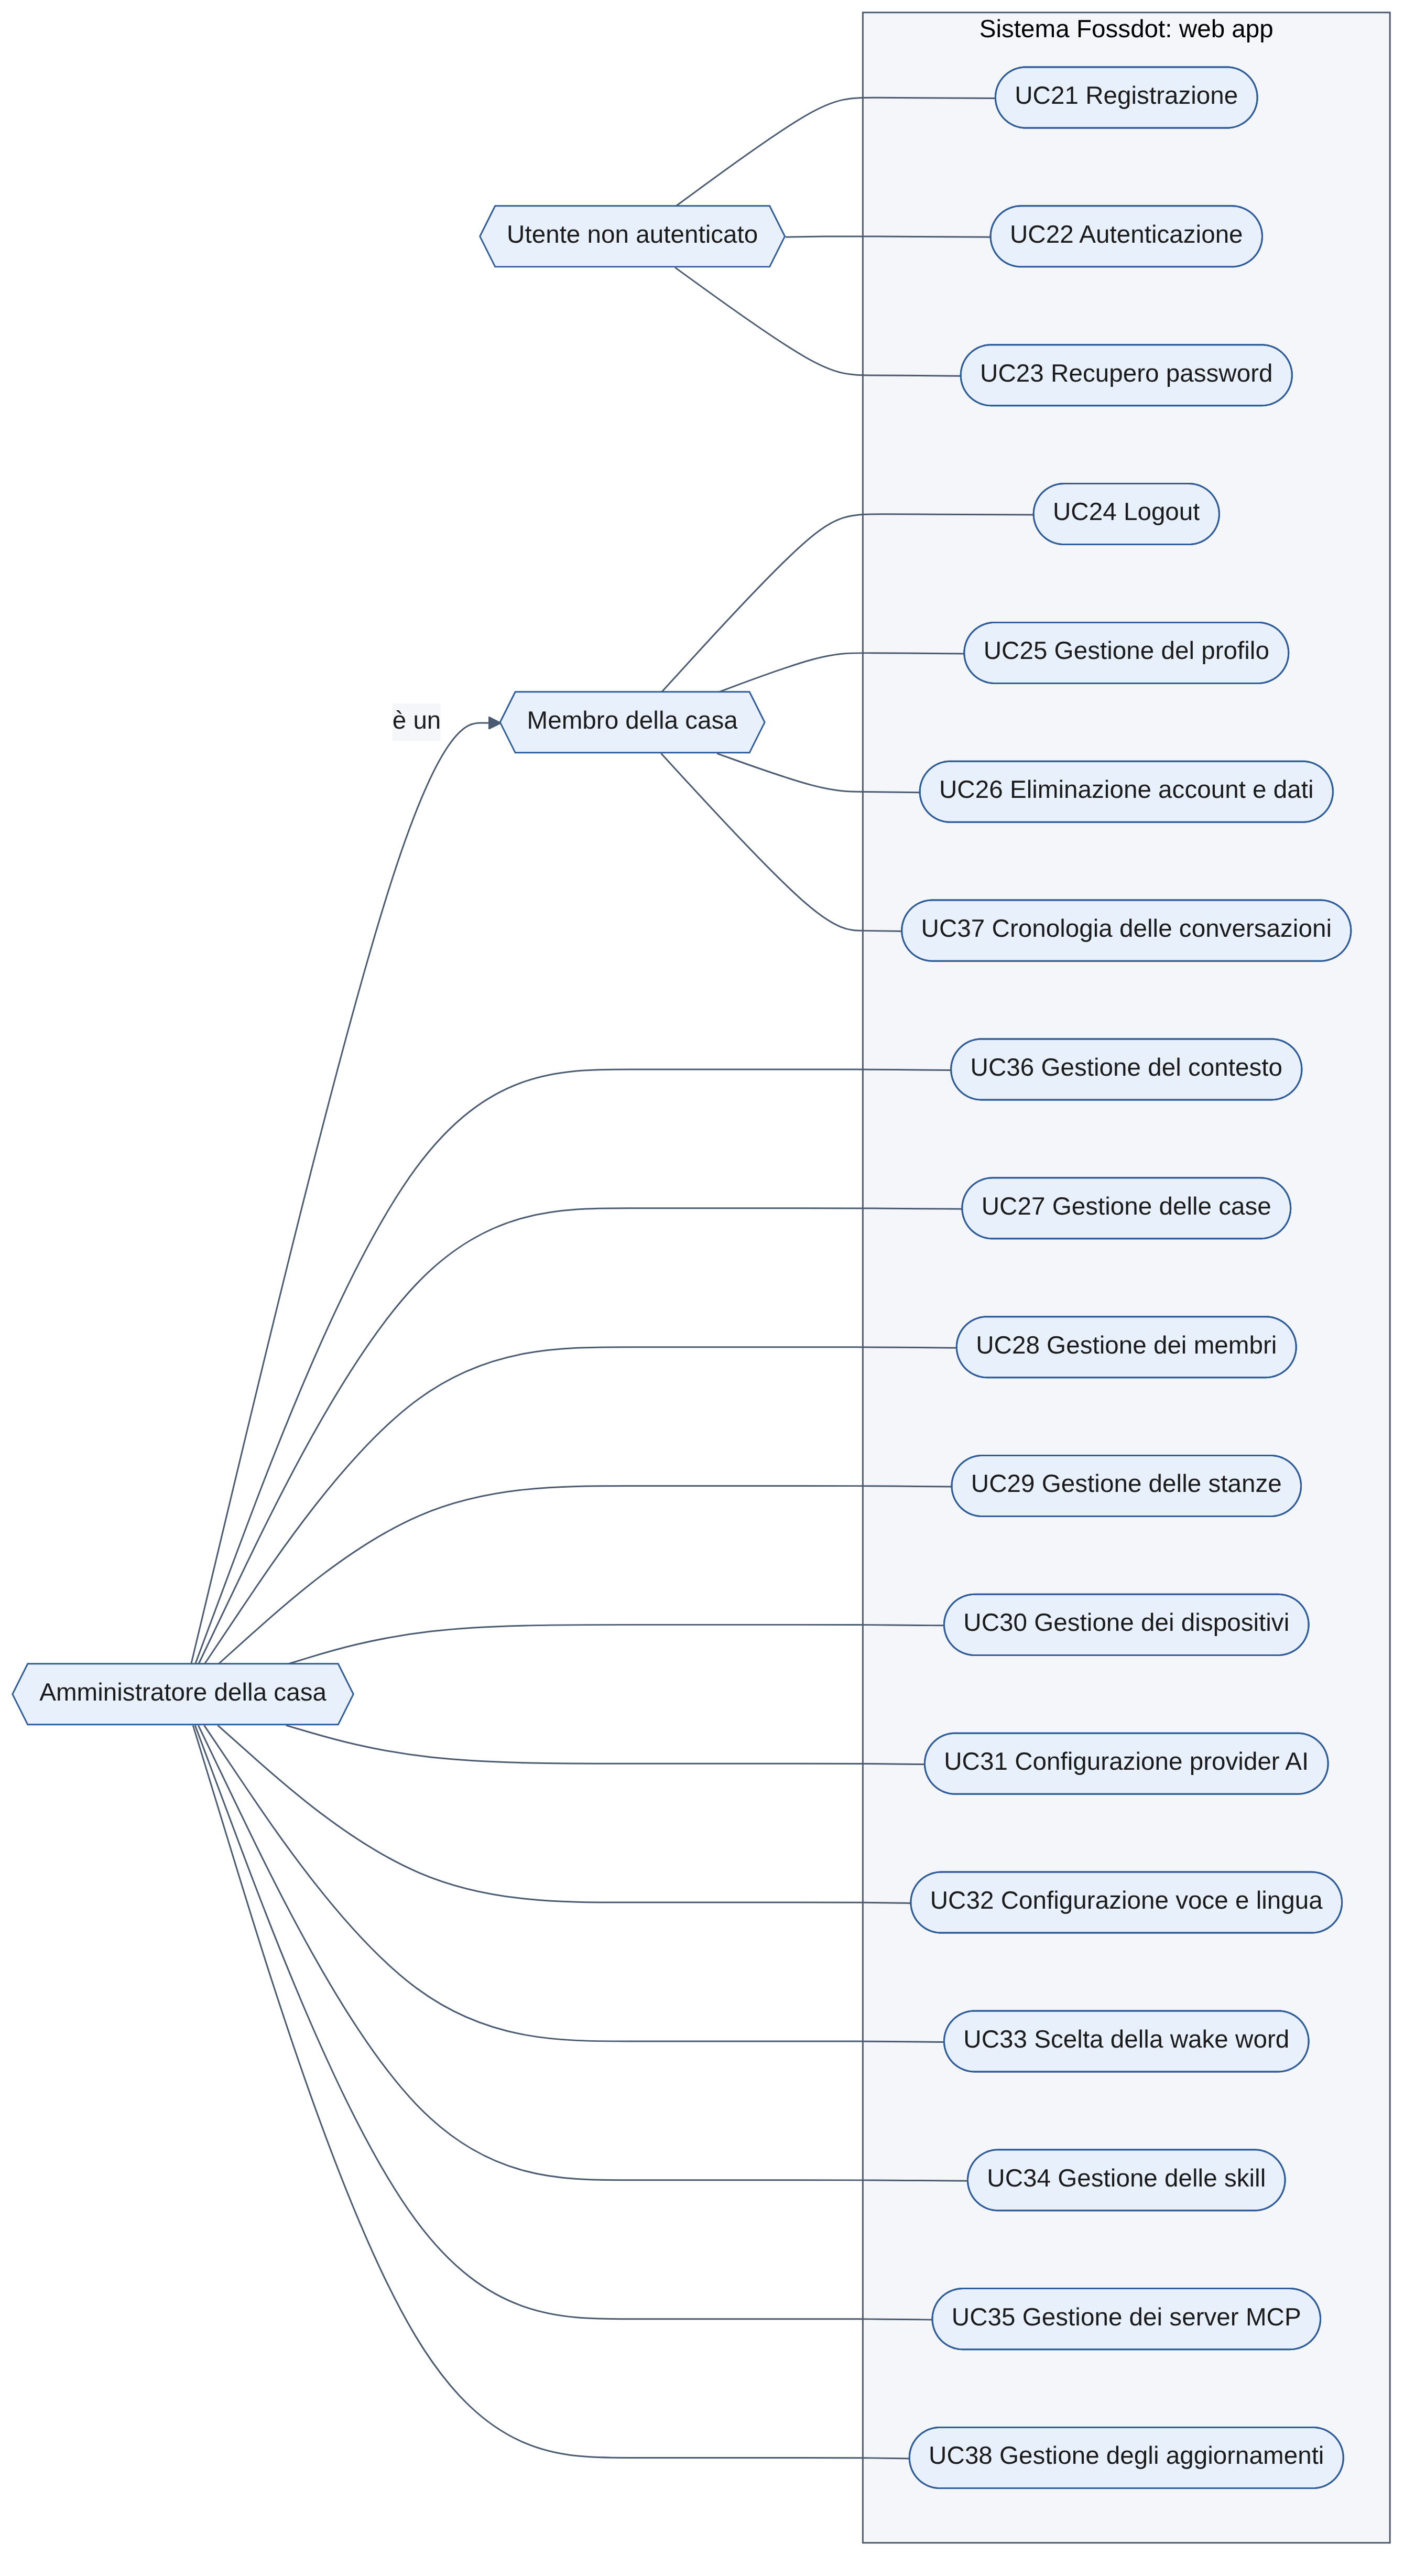
\includegraphics[width=\linewidth,height=0.62\textheight,keepaspectratio]{img_adr/12-uc-web.png}
\caption{Casi d'uso della web app (UC21--UC38)}
\end{figure}

Salvo diversa indicazione, nei casi d'uso di questa sezione la precondizione comune è che l'attore sia autenticato nella web app e appartenga alla casa su cui opera.

\subsubsection{UC21 -- Registrazione}
\begin{itemize}
\tightlist
\item \textbf{Attore primario:} Utente non autenticato.
\item \textbf{Precondizioni:} l'utente non ha una sessione attiva.
\item \textbf{Postcondizioni:} esiste un nuovo account, con una casa predefinita di cui l'utente è Amministratore.
\item \textbf{Scenario principale:}
\begin{enumerate}
\tightlist
\item L'utente inserisce nome, email e password.
\item Il sistema verifica i dati.
\item Il sistema crea l'account e la casa predefinita.
\end{enumerate}
\item \textbf{Estensioni:} al passo 2, dati non validi: UC21.1; email già registrata: UC21.2.
\item \textbf{Fonte:} Capitolato, Interna.
\end{itemize}

\paragraph{UC21.1 -- Dati di registrazione non validi}
\begin{itemize}
\tightlist
\item \textbf{Attore primario:} Utente non autenticato.
\item \textbf{Precondizioni:} l'email è malformata o la password non rispetta i criteri di robustezza.
\item \textbf{Postcondizioni:} nessun account è creato.
\item \textbf{Scenario principale:} il sistema indica il campo errato e il motivo; l'utente può correggerlo.
\item \textbf{Estende:} UC21, al passo 2.
\item \textbf{Fonte:} Interna.
\end{itemize}

\paragraph{UC21.2 -- Email già registrata}
\begin{itemize}
\tightlist
\item \textbf{Attore primario:} Utente non autenticato.
\item \textbf{Precondizioni:} esiste già un account con l'email indicata.
\item \textbf{Postcondizioni:} nessun account è creato.
\item \textbf{Scenario principale:} il sistema mostra un errore senza rivelare dati dell'account esistente.
\item \textbf{Estende:} UC21, al passo 2.
\item \textbf{Fonte:} Interna.
\end{itemize}

\subsubsection{UC22 -- Autenticazione}
\begin{itemize}
\tightlist
\item \textbf{Attore primario:} Utente non autenticato.
\item \textbf{Precondizioni:} l'utente ha un account e non ha una sessione attiva.
\item \textbf{Postcondizioni:} l'utente ha una sessione attiva e opera come Membro o Amministratore della propria casa.
\item \textbf{Scenario principale:}
\begin{enumerate}
\tightlist
\item L'utente inserisce email e password.
\item Il sistema verifica le credenziali.
\item Il sistema apre la sessione e mostra la casa.
\end{enumerate}
\item \textbf{Estensioni:} al passo 2, credenziali errate: UC22.1.
\item \textbf{Fonte:} Capitolato.
\end{itemize}

\paragraph{UC22.1 -- Credenziali errate}
\begin{itemize}
\tightlist
\item \textbf{Attore primario:} Utente non autenticato.
\item \textbf{Precondizioni:} email o password non corrispondono a un account.
\item \textbf{Postcondizioni:} nessuna sessione è aperta; il tentativo fallito è conteggiato.
\item \textbf{Scenario principale:} il sistema mostra un messaggio generico, senza indicare quale dato è sbagliato; dopo diversi tentativi falliti rallenta i successivi.
\item \textbf{Estende:} UC22, al passo 2.
\item \textbf{Fonte:} Interna.
\end{itemize}

\subsubsection{UC23 -- Recupero della password}
\begin{itemize}
\tightlist
\item \textbf{Attore primario:} Utente non autenticato.
\item \textbf{Precondizioni:} l'utente ha un account ma non ricorda la password.
\item \textbf{Postcondizioni:} l'account ha una nuova password; le sessioni precedenti non sono più valide.
\item \textbf{Scenario principale:}
\begin{enumerate}
\tightlist
\item L'utente chiede il recupero indicando l'email.
\item Il sistema invia un collegamento con scadenza.
\item L'utente apre il collegamento e imposta una nuova password.
\end{enumerate}
\item \textbf{Scenario alternativo:} il server \emph{self-hosted} non ha un servizio email; il recupero avviene da riga di comando sul server.
\item \textbf{Fonte:} Interna.
\end{itemize}

\subsubsection{UC24 -- Logout}
\begin{itemize}
\tightlist
\item \textbf{Attore primario:} Membro.
\item \textbf{Precondizioni:} il Membro ha una sessione attiva.
\item \textbf{Postcondizioni:} la sessione è chiusa e il suo token non è più valido.
\item \textbf{Scenario principale:} il Membro sceglie ``Esci''; il sistema invalida la sessione e mostra la pagina di accesso.
\item \textbf{Fonte:} Interna.
\end{itemize}

\subsubsection{UC25 -- Gestione del profilo}
\begin{itemize}
\tightlist
\item \textbf{Attore primario:} Membro.
\item \textbf{Postcondizioni:} nome, email o password del Membro sono aggiornati.
\item \textbf{Scenario principale:} il Membro modifica nome, email o password e conferma; il sistema salva i dati.
\item \textbf{Scenario alternativo:} per cambiare la password il Membro deve inserire quella attuale; se è errata la modifica è rifiutata.
\item \textbf{Fonte:} Interna.
\end{itemize}

\subsubsection{UC26 -- Eliminazione dell'account e dei dati}
\begin{itemize}
\tightlist
\item \textbf{Attore primario:} Membro.
\item \textbf{Postcondizioni:} l'account e i dati personali collegati (contesto, cronologia) non esistono più; ogni casa del Membro ha ancora almeno un Amministratore.
\item \textbf{Scenario principale:}
\begin{enumerate}
\tightlist
\item Il Membro chiede l'eliminazione dell'account.
\item Il sistema chiede conferma con la password.
\item Il sistema elimina l'account e i dati personali collegati e chiude la sessione.
\end{enumerate}
\item \textbf{Scenario alternativo:} al passo 2 il Membro è l'ultimo Amministratore di una casa con altri membri; il sistema chiede prima di nominare un nuovo Amministratore.
\item \textbf{Fonte:} Capitolato (GDPR), VE 13/11 (permanenza del dato).
\end{itemize}

\subsubsection{UC27 -- Gestione delle case}
\begin{itemize}
\tightlist
\item \textbf{Attore primario:} Amministratore.
\item \textbf{Postcondizioni:} l'elenco delle case dell'Amministratore riflette la modifica.
\item \textbf{Sottocasi:}
\begin{itemize}
\tightlist
\item \textbf{UC27.1 -- Creazione:} l'Amministratore indica nome, lingua e fuso orario; il sistema crea la casa e lo nomina Amministratore.
\item \textbf{UC27.2 -- Modifica:} l'Amministratore rinomina la casa o ne cambia le impostazioni.
\item \textbf{UC27.3 -- Eliminazione:} possibile solo se alla casa non sono associati dispositivi, previa conferma.
\end{itemize}
\item \textbf{Fonte:} VE 21/10 (``se possibile di più case'').
\end{itemize}

\subsubsection{UC28 -- Gestione dei membri}
\begin{itemize}
\tightlist
\item \textbf{Attore primario:} Amministratore.
\item \textbf{Postcondizioni:} l'elenco dei membri della casa e i loro ruoli riflettono la modifica; la casa ha almeno un Amministratore.
\item \textbf{Sottocasi:}
\begin{itemize}
\tightlist
\item \textbf{UC28.1 -- Invito:} l'Amministratore invita un utente con un collegamento o un codice; l'utente entra nella casa come Membro.
\item \textbf{UC28.2 -- Cambio di ruolo:} l'Amministratore cambia il ruolo di un membro (Membro $\leftrightarrow$ Amministratore).
\item \textbf{UC28.3 -- Rimozione:} il membro rimosso perde l'accesso alla casa.
\end{itemize}
\item \textbf{Fonte:} VE 21/10 (gestione di più utenti).
\end{itemize}

\subsubsection{UC29 -- Gestione delle stanze}
\begin{itemize}
\tightlist
\item \textbf{Attore primario:} Amministratore.
\item \textbf{Postcondizioni:} l'elenco delle stanze della casa riflette la modifica.
\item \textbf{Sottocasi:} \textbf{UC29.1 -- Creazione}; \textbf{UC29.2 -- Rinomina}; \textbf{UC29.3 -- Eliminazione} (i dispositivi della stanza restano senza stanza).
\item \textbf{Fonte:} Capitolato (stanze nella versione completa), Interna.
\end{itemize}

\subsubsection{UC30 -- Gestione dei dispositivi}
\begin{itemize}
\tightlist
\item \textbf{Attore primario:} Amministratore (il Membro può solo consultare l'elenco e il dettaglio).
\item \textbf{Postcondizioni:} la configurazione dei dispositivi della casa riflette la modifica.
\item \textbf{Sottocasi:}
\begin{itemize}
\tightlist
\item \textbf{UC30.1 -- Elenco:} nome, stanza, stato (in linea o no), versione del \emph{firmware}, ultimo contatto.
\item \textbf{UC30.2 -- Dettaglio:} configurazione corrente (\emph{provider}, voce, \emph{skill} abilitate).
\item \textbf{UC30.3 -- Rinomina.}
\item \textbf{UC30.4 -- Assegnazione a una stanza:} un dispositivo appartiene al più a una stanza.
\item \textbf{UC30.5 -- Dissociazione:} le credenziali del dispositivo sono revocate e il dispositivo non può più collegarsi al server.
\item \textbf{UC30.6 -- Aggiunta:} avvia UC17.
\end{itemize}
\item \textbf{Fonte:} Capitolato, VE 21/10.
\end{itemize}

\subsubsection{UC31 -- Configurazione del provider AI}
\begin{itemize}
\tightlist
\item \textbf{Attore primario:} Amministratore. \textbf{Servizi coinvolti:} \emph{provider} AI.
\item \textbf{Postcondizioni:} la casa (o il dispositivo) ha un \emph{provider} AI e un modello assegnati, validi dalla richiesta successiva.
\item \textbf{Scenario principale:}
\begin{enumerate}
\tightlist
\item L'Amministratore sceglie il \emph{provider} da un elenco predefinito (UC31.1) o indica un \emph{endpoint} personalizzato (UC31.2).
\item L'Amministratore inserisce la chiave API (UC31.3).
\item L'Amministratore sceglie il modello (UC31.4).
\item Il sistema verifica la connessione (UC31.6).
\item L'Amministratore assegna il \emph{provider} alla casa o a un dispositivo (UC31.5) e salva.
\end{enumerate}
\item \textbf{Sottocasi:}
\begin{itemize}
\tightlist
\item \textbf{UC31.1 -- Scelta da elenco predefinito:} OpenAI, Anthropic, OpenRouter, DeepSeek, Ollama.
\item \textbf{UC31.2 -- Endpoint personalizzato:} URL compatibile OpenAI (ad esempio un Ollama sulla rete di casa).
\item \textbf{UC31.3 -- Chiave API:} inserita una volta, poi mostrata solo mascherata.
\item \textbf{UC31.4 -- Scelta del modello:} dall'elenco esposto dal \emph{provider} o inserito a mano.
\item \textbf{UC31.5 -- Assegnazione:} \emph{provider} predefinito della casa e, se serve, \emph{provider} specifico per un dispositivo.
\item \textbf{UC31.6 -- Verifica della connessione:} il sistema prova una richiesta minima e mostra l'esito.
\item \textbf{UC31.8 -- Più provider configurati:} più \emph{provider} configurati insieme, commutabili senza riavviare il server.
\end{itemize}
\item \textbf{Estensioni:} al passo 4, verifica non riuscita: UC31.7.
\item \textbf{Fonte:} Capitolato (MVP: \emph{provider} configurabile; versione completa: più \emph{provider} commutabili), VE 21/10, VE 13/11 (modello configurabile per contenere i costi).
\end{itemize}

\paragraph{UC31.7 -- Verifica del provider non riuscita}
\begin{itemize}
\tightlist
\item \textbf{Attore primario:} Amministratore.
\item \textbf{Precondizioni:} la richiesta di prova al \emph{provider} fallisce (indirizzo non raggiungibile, chiave non valida, modello inesistente, tempo scaduto).
\item \textbf{Postcondizioni:} la configurazione precedente resta in uso; la web app mostra il motivo dell'errore.
\item \textbf{Scenario principale:} il sistema mostra il motivo del fallimento e chiede all'Amministratore se correggere i dati o salvare comunque la configurazione senza assegnarla.
\item \textbf{Estende:} UC31, al passo 4.
\item \textbf{Fonte:} Interna.
\end{itemize}

\subsubsection{UC32 -- Configurazione di voce e lingua}
\begin{itemize}
\tightlist
\item \textbf{Attore primario:} Amministratore.
\item \textbf{Postcondizioni:} lingua e voce della sintesi sono aggiornate per la casa o per il dispositivo e valgono dalla richiesta successiva.
\item \textbf{Scenario principale:} l'Amministratore sceglie per la casa o per un dispositivo la lingua e la voce della sintesi vocale e salva. I motori di trascrizione e di sintesi sono quelli del server e non si scelgono dalla web app.
\item \textbf{Fonte:} Interna.
\end{itemize}

\subsubsection{UC33 -- Scelta della wake word}
\begin{itemize}
\tightlist
\item \textbf{Attore primario:} Amministratore.
\item \textbf{Postcondizioni:} il dispositivo usa la nuova \emph{wake word}.
\item \textbf{Scenario principale:} l'Amministratore sceglie la \emph{wake word} da un elenco di modelli disponibili; il dispositivo la riceve con la configurazione o con un aggiornamento.
\item \textbf{Fonte:} Interna, da chiedere a Uranion.
\end{itemize}

\subsubsection{UC34 -- Gestione delle skill}
\begin{itemize}
\tightlist
\item \textbf{Attore primario:} Amministratore.
\item \textbf{Postcondizioni:} l'insieme delle \emph{skill} installate, la loro configurazione e la loro abilitazione per dispositivo riflettono la modifica.
\item \textbf{Sottocasi:}
\begin{itemize}
\tightlist
\item \textbf{UC34.1 -- Elenco:} \emph{skill} installate con nome, descrizione, versione e dispositivi su cui sono attive.
\item \textbf{UC34.2 -- Caricamento:} l'Amministratore carica il file della \emph{skill} nel formato standard; il sistema la valida e la installa.
\item \textbf{UC34.4 -- Configurazione dei parametri:} ad esempio città predefinita per il meteo, chiave di un servizio.
\item \textbf{UC34.5 -- Abilitazione per dispositivo.}
\item \textbf{UC34.6 -- Rimozione.}
\item \textbf{UC34.7 -- Autorizzazione esterna:} la \emph{skill} reindirizza a un sito esterno e riceve una \emph{callback} (predisposizione per l'IoT, VE 21/10).
\end{itemize}
\item \textbf{Estensioni:} in UC34.2, file non valido: UC34.3.
\item \textbf{Fonte:} Capitolato, VE 21/10.
\end{itemize}

\paragraph{UC34.3 -- Formato della skill non valido}
\begin{itemize}
\tightlist
\item \textbf{Attore primario:} Amministratore.
\item \textbf{Precondizioni:} il file caricato non rispetta il formato standard delle \emph{skill}.
\item \textbf{Postcondizioni:} la \emph{skill} non è installata.
\item \textbf{Scenario principale:} il sistema rifiuta il file e indica l'errore trovato.
\item \textbf{Estende:} UC34.2, alla validazione.
\item \textbf{Fonte:} Interna.
\end{itemize}

\subsubsection{UC35 -- Gestione dei server MCP}
\begin{itemize}
\tightlist
\item \textbf{Attore primario:} Amministratore. \textbf{Servizi coinvolti:} server MCP.
\item \textbf{Postcondizioni:} l'insieme dei server MCP configurati e degli strumenti offerti al modello riflette la modifica.
\item \textbf{Sottocasi:}
\begin{itemize}
\tightlist
\item \textbf{UC35.1 -- Aggiunta:} nome, URL o comando, eventuale autenticazione.
\item \textbf{UC35.2 -- Visualizzazione e selezione degli strumenti} esposti dal server.
\item \textbf{UC35.3 -- Rimozione.}
\end{itemize}
\item \textbf{Estensioni:} server non raggiungibile: UC35.4.
\item \textbf{Fonte:} Capitolato.
\end{itemize}

\paragraph{UC35.4 -- Server MCP non raggiungibile}
\begin{itemize}
\tightlist
\item \textbf{Attore primario:} Amministratore.
\item \textbf{Precondizioni:} un server MCP configurato non risponde.
\item \textbf{Postcondizioni:} il server MCP è segnato in errore e i suoi strumenti non sono offerti al modello.
\item \textbf{Scenario principale:} la web app mostra lo stato di errore del server MCP; l'Amministratore può correggerne i dati o rimuoverlo.
\item \textbf{Estende:} UC35.1 e UC35.2.
\item \textbf{Fonte:} Interna.
\end{itemize}

\subsubsection{UC36 -- Gestione del contesto}
\begin{itemize}
\tightlist
\item \textbf{Attore primario:} Amministratore.
\item \textbf{Postcondizioni:} il testo di contesto del dispositivo è aggiornato o cancellato e vale dalla richiesta successiva.
\item \textbf{Scenario principale:} l'Amministratore apre il contesto (testo Markdown) di un dispositivo, lo modifica o lo cancella e salva.
\item \textbf{Fonte:} VE 13/11.
\end{itemize}

\subsubsection{UC37 -- Cronologia delle conversazioni}
\begin{itemize}
\tightlist
\item \textbf{Attore primario:} Membro.
\item \textbf{Precondizioni:} la conservazione delle trascrizioni è attiva per il dispositivo.
\item \textbf{Postcondizioni:} le trascrizioni scelte sono state consultate o cancellate.
\item \textbf{Scenario principale:} il Membro consulta le trascrizioni recenti di un dispositivo e può cancellarle singolarmente o tutte.
\item \textbf{Scenario alternativo:} l'Amministratore disattiva la conservazione o ne cambia la durata massima.
\item \textbf{Fonte:} VE 13/11 (indagine sulla permanenza del dato), Capitolato (GDPR). Da confermare con Uranion.
\end{itemize}

\subsubsection{UC38 -- Gestione degli aggiornamenti del firmware}
\begin{itemize}
\tightlist
\item \textbf{Attore primario:} Amministratore.
\item \textbf{Postcondizioni:} l'aggiornamento è avviato, oppure è cambiata l'impostazione degli aggiornamenti automatici.
\item \textbf{Scenario principale:} l'Amministratore vede la versione installata su ogni dispositivo e quella disponibile e avvia l'aggiornamento (UC20).
\item \textbf{Scenario alternativo:} l'Amministratore attiva o disattiva gli aggiornamenti automatici.
\item \textbf{Fonte:} Capitolato.
\end{itemize}

\subsection{Priorità e fasi dei casi d'uso}\label{sec:fasi}

La tabella riporta, per ogni caso d'uso, la priorità e la fase in cui il gruppo prevede di realizzarlo: \emph{PoC} (\emph{Proof of Concept}, gennaio 2027) oppure \emph{MVP} (26/03/2027). Nessun caso d'uso è rimandato a dopo l'\emph{MVP}. La divisione va confermata con \emph{Uranion} (Q2).

\begin{center}
\begin{tabularx}{0.75\linewidth}{X>{\centering\arraybackslash}p{1.4cm}>{\centering\arraybackslash}p{1.4cm}>{\centering\arraybackslash}p{1.4cm}>{\centering\arraybackslash}p{1.4cm}}
\rowcolor{bfblue}\thc{Fase} & \thc{Obb} & \thc{Des} & \thc{Opz} & \thc{Totale} \\
PoC & 20 & 6 & 0 & \textbf{26} \rl
MVP & 20 & 41 & 3 & \textbf{64} \rl
\textbf{Totale} & \textbf{40} & \textbf{47} & \textbf{3} & \textbf{90} \rl
\end{tabularx}
\end{center}

I casi d'uso sono 90: 38 principali e 52 sottocasi. Nel \emph{PoC} ci sono 14 casi d'uso principali, nell'\emph{MVP} 24.

\begin{longtable}{>{\raggedright\arraybackslash}p{\dimexpr(\linewidth-8\tabcolsep)*150/1000\relax}>{\raggedright\arraybackslash}p{\dimexpr(\linewidth-8\tabcolsep)*580/1000\relax}>{\centering\arraybackslash}p{\dimexpr(\linewidth-8\tabcolsep)*130/1000\relax}>{\centering\arraybackslash}p{\dimexpr(\linewidth-8\tabcolsep)*140/1000\relax}}
\rowcolor{bfblue}\thc{Caso d'uso} & \thc{Nome} & \thc{Priorità} & \thc{Fase} \\
\endfirsthead
\rowcolor{bfblue}\thc{Caso d'uso} & \thc{Nome} & \thc{Priorità} & \thc{Fase} \\
\endhead
\textbf{UC1} & \textbf{Attivazione dell'ascolto} & Obb & PoC \rl
\hspace{1em}UC1.1 & Attivazione con wake word & Obb & PoC \rl
\hspace{1em}UC1.2 & Attivazione con pulsante (push-to-talk) & Des & PoC \rl
\textbf{UC2} & \textbf{Richiesta vocale con risposta} & Obb & PoC \rl
\hspace{1em}UC2.1 & Acquisizione della richiesta e rilevamento della fine & Obb & PoC \rl
\hspace{1em}UC2.2 & Ricezione della risposta vocale & Obb & PoC \rl
\textbf{UC3} & \textbf{Nessun parlato dopo l'attivazione} & Obb & PoC \rl
\textbf{UC4} & \textbf{Richiesta non compresa} & Obb & PoC \rl
\textbf{UC5} & \textbf{Interruzione della risposta con ``Ehi Fossdot''} & Obb & PoC \rl
\textbf{UC6} & \textbf{Sostituzione della richiesta in corso} & Des & PoC \rl
\textbf{UC7} & \textbf{Servizio non disponibile} & Obb & PoC \rl
\textbf{UC8} & \textbf{Mute dei microfoni} & Obb & PoC \rl
\textbf{UC9} & \textbf{Regolazione del volume} & Des & MVP \rl
\hspace{1em}UC9.1 & Impostazione del volume con i tasti & Des & PoC \rl
\hspace{1em}UC9.2 & Impostazione del volume a voce & Des & MVP \rl
\textbf{UC10} & \textbf{Invocazione di una skill} & Obb & MVP \rl
\hspace{1em}UC10.1 & Errore nell'esecuzione di una skill & Des & MVP \rl
\hspace{1em}UC10.2 & Richiesta di un dato mancante & Des & MVP \rl
\hspace{1em}UC10.3 & Conferma di un'azione con effetti esterni & Obb & MVP \rl
\textbf{UC11} & \textbf{Attività multi-step (agent)} & Des & MVP \rl
\textbf{UC12} & \textbf{Uso di uno strumento MCP} & Obb & MVP \rl
\textbf{UC13} & \textbf{Aggiornamento del contesto a voce} & Opz & MVP \rl
\textbf{UC14} & \textbf{Chiamata tra dispositivi} & Des & MVP \rl
\hspace{1em}UC14.1 & Avvio di una chiamata & Des & MVP \rl
\hspace{1em}UC14.2 & Ricezione di una chiamata & Des & MVP \rl
\hspace{1em}UC14.3 & Termine della chiamata & Des & MVP \rl
\hspace{1em}UC14.4 & Dispositivo da chiamare non disponibile & Des & MVP \rl
\textbf{UC15} & \textbf{Messaggio vocale verso un altro dispositivo} & Des & MVP \rl
\textbf{UC16} & \textbf{Primo avvio e configurazione del Wi-Fi} & Obb & PoC \rl
\hspace{1em}UC16.1 & Rete o password errate & Obb & PoC \rl
\textbf{UC17} & \textbf{Aggiunta del dispositivo alla casa} & Obb & MVP \rl
\textbf{UC18} & \textbf{Cambio della rete Wi-Fi} & Des & MVP \rl
\textbf{UC19} & \textbf{Ripristino di fabbrica} & Des & PoC \rl
\textbf{UC20} & \textbf{Aggiornamento del firmware} & Des & MVP \rl
\hspace{1em}UC20.1 & Ritorno alla versione precedente & Des & MVP \rl
\textbf{UC21} & \textbf{Registrazione} & Obb & PoC \rl
\hspace{1em}UC21.1 & Dati di registrazione non validi & Obb & PoC \rl
\hspace{1em}UC21.2 & Email già registrata & Obb & PoC \rl
\textbf{UC22} & \textbf{Autenticazione} & Obb & PoC \rl
\hspace{1em}UC22.1 & Credenziali errate & Obb & PoC \rl
\textbf{UC23} & \textbf{Recupero della password} & Des & MVP \rl
\textbf{UC24} & \textbf{Logout} & Obb & PoC \rl
\textbf{UC25} & \textbf{Gestione del profilo} & Des & MVP \rl
\textbf{UC26} & \textbf{Eliminazione dell'account e dei dati} & Obb & MVP \rl
\textbf{UC27} & \textbf{Gestione delle case} & Des & MVP \rl
\hspace{1em}UC27.1 & Creazione & Des & MVP \rl
\hspace{1em}UC27.2 & Modifica & Des & MVP \rl
\hspace{1em}UC27.3 & Eliminazione & Des & MVP \rl
\textbf{UC28} & \textbf{Gestione dei membri} & Des & MVP \rl
\hspace{1em}UC28.1 & Invito & Des & MVP \rl
\hspace{1em}UC28.2 & Cambio di ruolo & Des & MVP \rl
\hspace{1em}UC28.3 & Rimozione & Des & MVP \rl
\textbf{UC29} & \textbf{Gestione delle stanze} & Des & MVP \rl
\hspace{1em}UC29.1 & Creazione & Des & MVP \rl
\hspace{1em}UC29.2 & Rinomina & Des & MVP \rl
\hspace{1em}UC29.3 & Eliminazione & Des & MVP \rl
\textbf{UC30} & \textbf{Gestione dei dispositivi} & Obb & MVP \rl
\hspace{1em}UC30.1 & Elenco & Obb & MVP \rl
\hspace{1em}UC30.2 & Dettaglio & Des & MVP \rl
\hspace{1em}UC30.3 & Rinomina & Obb & MVP \rl
\hspace{1em}UC30.4 & Assegnazione a una stanza & Des & MVP \rl
\hspace{1em}UC30.5 & Dissociazione & Obb & MVP \rl
\hspace{1em}UC30.6 & Aggiunta & Obb & MVP \rl
\textbf{UC31} & \textbf{Configurazione del provider AI} & Obb & PoC \rl
\hspace{1em}UC31.1 & Scelta da elenco predefinito & Obb & MVP \rl
\hspace{1em}UC31.2 & Endpoint personalizzato & Obb & MVP \rl
\hspace{1em}UC31.3 & Chiave API & Obb & PoC \rl
\hspace{1em}UC31.4 & Scelta del modello & Obb & MVP \rl
\hspace{1em}UC31.5 & Assegnazione & Des & MVP \rl
\hspace{1em}UC31.6 & Verifica della connessione & Des & PoC \rl
\hspace{1em}UC31.7 & Verifica del provider non riuscita & Des & PoC \rl
\hspace{1em}UC31.8 & Più provider configurati & Des & MVP \rl
\textbf{UC32} & \textbf{Configurazione di voce e lingua} & Obb & MVP \rl
\textbf{UC33} & \textbf{Scelta della wake word} & Opz & MVP \rl
\textbf{UC34} & \textbf{Gestione delle skill} & Des & MVP \rl
\hspace{1em}UC34.1 & Elenco & Des & MVP \rl
\hspace{1em}UC34.2 & Caricamento & Des & MVP \rl
\hspace{1em}UC34.3 & Formato della skill non valido & Des & MVP \rl
\hspace{1em}UC34.4 & Configurazione dei parametri & Des & MVP \rl
\hspace{1em}UC34.5 & Abilitazione per dispositivo & Des & MVP \rl
\hspace{1em}UC34.6 & Rimozione & Des & MVP \rl
\hspace{1em}UC34.7 & Autorizzazione esterna & Opz & MVP \rl
\textbf{UC35} & \textbf{Gestione dei server MCP} & Obb & MVP \rl
\hspace{1em}UC35.1 & Aggiunta & Obb & MVP \rl
\hspace{1em}UC35.2 & Visualizzazione e selezione degli strumenti & Obb & MVP \rl
\hspace{1em}UC35.3 & Rimozione & Obb & MVP \rl
\hspace{1em}UC35.4 & Server MCP non raggiungibile & Obb & MVP \rl
\textbf{UC36} & \textbf{Gestione del contesto} & Des & MVP \rl
\textbf{UC37} & \textbf{Cronologia delle conversazioni} & Obb & MVP \rl
\textbf{UC38} & \textbf{Gestione degli aggiornamenti del firmware} & Des & MVP \rl
\end{longtable}

Note sulla divisione:
\begin{itemize}
\tightlist
\item \textbf{UC9.} UC9.1 (volume con i tasti) è nel \emph{PoC} solo se il gruppo salda i tasti, altrimenti passa all'\emph{MVP}. Per questo UC9 principale è nell'\emph{MVP}; se i tasti vengono saldati, UC9 passa nel \emph{PoC}.
\item \textbf{UC16 e UC17.} UC16 è nel \emph{PoC} ma include UC17 (aggiunta del dispositivo alla casa, passo 6), che è nell'\emph{MVP}. Nel \emph{PoC} il passo 6 si salta, oppure UC17 va anticipato insieme agli account (UC21, UC22, UC24).
\item \textbf{UC31.} Nel \emph{PoC} è previsto un solo \emph{provider} fisso; la scelta da elenco, l'\emph{endpoint} personalizzato, la scelta del modello, l'assegnazione e più \emph{provider} insieme (UC31.1, UC31.2, UC31.4, UC31.5, UC31.8) sono nell'\emph{MVP}.
\item \textbf{Sottocasi di UC14, UC21 e UC22.} Seguono il loro caso principale.
\end{itemize}

\subsection{Modello di dominio}

Le entità che i casi d'uso manipolano, utili per verificare che non manchino casi di gestione. \ph{Modello da verificare con il gruppo.}

\begin{figure}[H]
\centering
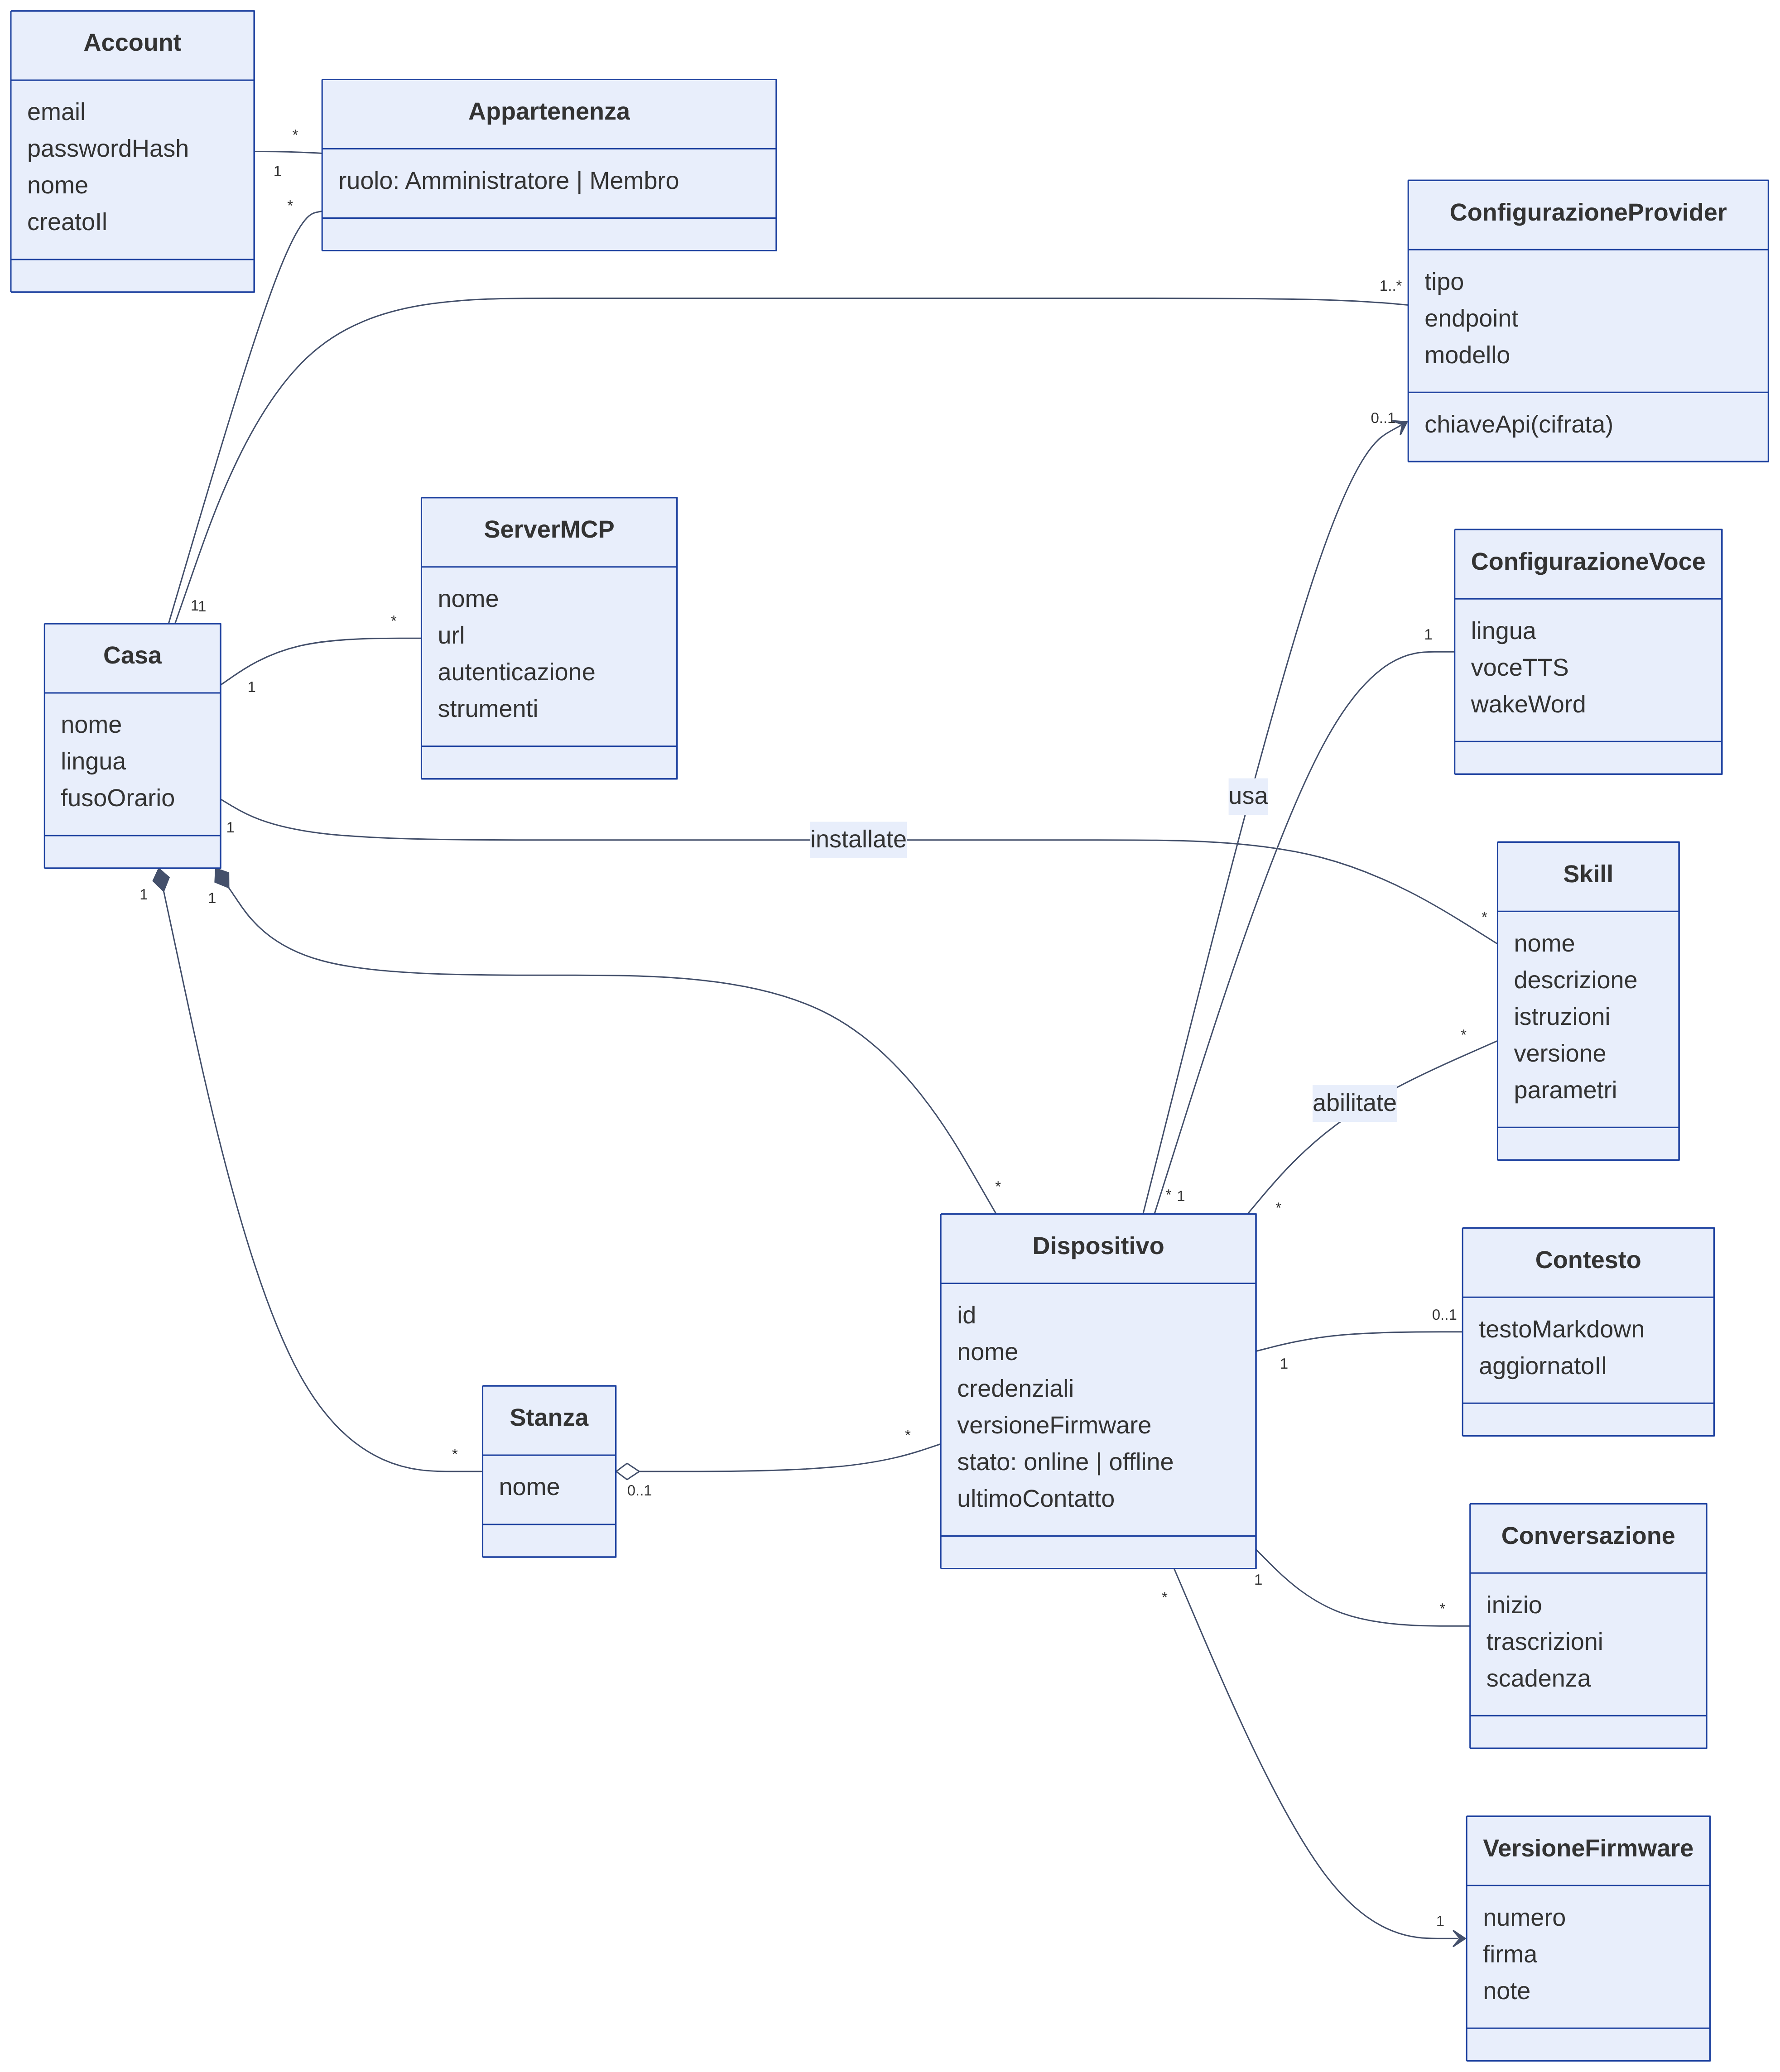
\includegraphics[width=\linewidth,height=0.62\textheight,keepaspectratio]{img_adr/14-dominio.png}
\caption{Modello di dominio}
\end{figure}

\section{Requisiti}\label{sec:requisiti}

Legenda della colonna \textbf{Comp.}: D = dispositivo (\emph{firmware}), H = \emph{hardware}, S = server di bridging, W = web app, T = trasversale. La colonna \textbf{Ver.} indica il metodo di verifica (T test, D dimostrazione, I ispezione, A analisi).

\subsection{Requisiti funzionali}

\subsubsection{Interazione vocale}

\begin{longtable}{>{\raggedright\arraybackslash}p{\dimexpr(\linewidth-10\tabcolsep)*140/1000\relax}>{\raggedright\arraybackslash}p{\dimexpr(\linewidth-10\tabcolsep)*530/1000\relax}>{\raggedright\arraybackslash}p{\dimexpr(\linewidth-10\tabcolsep)*175/1000\relax}>{\raggedright\arraybackslash}p{\dimexpr(\linewidth-10\tabcolsep)*85/1000\relax}>{\centering\arraybackslash}p{\dimexpr(\linewidth-10\tabcolsep)*70/1000\relax}}
\rowcolor{bfblue}\thc{Codice} & \thc{Descrizione} & \thc{Fonti} & \thc{Comp.} & \thc{Ver.} \\
\endfirsthead
\rowcolor{bfblue}\thc{Codice} & \thc{Descrizione} & \thc{Fonti} & \thc{Comp.} & \thc{Ver.} \\
\endhead
RF-1-Obb & Il dispositivo deve riconoscere la \emph{wake word} in locale, in modo continuo, senza inviare audio all'esterno. & Capitolato, VE 21/10, UC1.1 & D & T \rl
RF-2-Des & L'utente deve poter attivare l'ascolto premendo un pulsante (\emph{push-to-talk}). & Capitolato, UC1.2 & D, H & D \rl
RF-3-Obb & All'attivazione il dispositivo deve emettere un suono breve e mostrare lo stato ``in ascolto'' sui LED. & UC1 & D & D \rl
RF-4-Obb & Dopo l'attivazione il dispositivo deve acquisire l'audio della richiesta dai microfoni. & Capitolato, UC2.1 & D & T \rl
RF-5-Obb & Il dispositivo deve inviare l'audio al server in \emph{streaming}, a frame di durata fissa, solo dopo l'attivazione. & Capitolato, VE 21/10, UC2 & D, S & T \rl
RF-6-Obb & Il protocollo tra dispositivo e server deve distinguere i dati audio dai messaggi di controllo (inizio sessione, fine ascolto, annullamento, fine risposta, stato, comandi LED). & VE 13/11, UC2, UC5 & D, S & T \rl
RF-7-Obb & Il dispositivo deve mantenere sempre aperta una connessione WebSocket bidirezionale con il server, usata anche quando il dispositivo è inattivo per ricevere comandi e avvisi (ad esempio un nuovo \emph{firmware}). & VE 13/11, Interna & D, S & T \rl
RF-8-Obb & Il server deve rilevare la fine della richiesta in base al silenzio e alla durata massima. & UC2.1, Interna & S & T \rl
RF-9-Obb & Il server deve trascrivere l'audio della richiesta in testo (STT). & Capitolato, UC2 & S & T \rl
RF-10-Obb & Il server deve inviare la trascrizione al \emph{provider} AI configurato per il dispositivo, insieme al prompt di sistema. & Capitolato, UC2 & S & T \rl
RF-11-Obb & Il server deve convertire la risposta del modello in audio (TTS). & Capitolato, UC2 & S & T \rl
RF-12-Obb & Il server deve inviare l'audio della risposta in \emph{streaming}, iniziando prima che la risposta del modello sia completa. & UC2.2, Interna & S & T \rl
RF-13-Obb & Il dispositivo deve riprodurre l'audio della risposta mostrando lo stato ``risposta'' sui LED. & Capitolato, UC2 & D & D \rl
RF-14-Obb & Se l'utente non parla entro il tempo di attesa, il sistema deve chiudere la sessione senza contattare il \emph{provider}. & UC3 & S & T \rl
RF-15-Obb & Se la trascrizione è vuota o non valida, il dispositivo deve riprodurre un messaggio di mancata comprensione. & UC4 & S & T \rl
RF-16-Obb & Se il \emph{provider}, l'STT o il TTS falliscono o superano il tempo massimo, il dispositivo deve riprodurre un messaggio vocale di errore. & UC7 & S, D & T \rl
RF-17-Obb & Se il server non è raggiungibile, il dispositivo deve segnalarlo con i LED e con un suono memorizzato sul dispositivo. & UC7 & D & T \rl
RF-18-Des & Il server deve mantenere il contesto della conversazione tra richieste ravvicinate dello stesso dispositivo (dialogo multi-turno). & UC2, Interna & S & T \rl
RF-20-Obb & Durante la riproduzione il dispositivo deve continuare a riconoscere in locale la \emph{wake word} e, se la riconosce, fermare subito l'audio; non è prevista una parola ``stop'' separata. & VE 13/11, UC5 & D & T \rl
RF-21-Obb & Ricevuto l'annullamento, il server deve interrompere la generazione del modello e la sintesi e scartare l'audio residuo. & VE 13/11, UC5 & S & T \rl
RF-22-Des & Una nuova \emph{wake word} durante l'elaborazione o la risposta deve annullare la richiesta in corso e avviarne una nuova. & VE 13/11, UC6 & D, S & T \rl
RF-23-Des & Il dispositivo non deve attivarsi né interrompersi a causa della propria voce (cancellazione dell'eco). & VE 21/10, VE 13/11 & D, H & T \rl
RF-24-Obb & Il server deve applicare un tempo massimo a ogni chiamata verso \emph{provider}, STT e TTS. & UC7 & S & T \rl
RF-25-Obb & Il prompt di sistema deve chiedere al modello risposte adatte alla voce: brevi, senza formattazione, nella lingua configurata. & Interna & S & T \rl
RF-26-Obb & I LED devono indicare in modo distinguibile almeno questi stati: da configurare, connessione, inattivo, in ascolto, elaborazione, risposta, muto, errore, non connesso, aggiornamento, chiamata. & Capitolato, UC1, UC8, UC16 & D, H & D \rl
RF-27-Obb & Il dispositivo deve avere un comando fisico per disattivare e riattivare i microfoni. & Interna, UC8 & D, H & D \rl
RF-28-Obb & In mute il dispositivo non deve acquisire né inviare audio, \emph{wake word} compresa, e deve mostrare un LED dedicato. & UC8 & D & T \rl
RF-29-Des & Il pulsante azione deve permettere di interrompere la risposta, attivare l'ascolto e chiudere una chiamata. & UC1.2, UC5, UC14.3 & D, H & D \rl
RF-30-Des & L'utente deve poter regolare il volume con i tasti del dispositivo. & UC9.1 & D, H & D \rl
RF-31-Obb & Il dispositivo deve riprodurre suoni di riscontro per attivazione, errore e conferma. & UC1, UC7 & D & D \rl
RF-32-Des & Il livello del volume deve restare memorizzato dopo un riavvio. & UC9 & D & T \rl
RF-33-Des & L'utente deve poter regolare il volume a voce. & UC9.2 & D, S & D \rl
\end{longtable}

\subsubsection{Onboarding, connessione e stato}

\begin{longtable}{>{\raggedright\arraybackslash}p{\dimexpr(\linewidth-10\tabcolsep)*140/1000\relax}>{\raggedright\arraybackslash}p{\dimexpr(\linewidth-10\tabcolsep)*530/1000\relax}>{\raggedright\arraybackslash}p{\dimexpr(\linewidth-10\tabcolsep)*175/1000\relax}>{\raggedright\arraybackslash}p{\dimexpr(\linewidth-10\tabcolsep)*85/1000\relax}>{\centering\arraybackslash}p{\dimexpr(\linewidth-10\tabcolsep)*70/1000\relax}}
\rowcolor{bfblue}\thc{Codice} & \thc{Descrizione} & \thc{Fonti} & \thc{Comp.} & \thc{Ver.} \\
\endfirsthead
\rowcolor{bfblue}\thc{Codice} & \thc{Descrizione} & \thc{Fonti} & \thc{Comp.} & \thc{Ver.} \\
\endhead
RF-40-Obb & Al primo avvio, o dopo un ripristino, il dispositivo deve entrare in modalità configurazione e segnalarlo con i LED. & Capitolato, VE 21/10, UC16 & D & D \rl
RF-41-Obb & In modalità configurazione il dispositivo deve creare una propria rete Wi-Fi temporanea; collegandosi a questa rete da un telefono o da un PC, senza installare \emph{software}, l'utente deve trovare una pagina di configurazione (\emph{captive portal}) in cui inserire rete e password del Wi-Fi di casa. & VE 21/10, UC16 & D & D \rl
RF-42-Obb & L'utente deve poter indicare l'indirizzo del server a cui collegare il dispositivo. & UC16, Interna (\emph{self-hosted}) & D & T \rl
RF-43-Obb & Un dispositivo connesso al server e non ancora aggiunto a una casa deve comparire nella web app, e l'Amministratore deve poterlo aggiungere a una delle sue case o rifiutarlo. & UC17, UC30.6 & W, S & T \rl
RF-44-Obb & Il server deve assegnare al dispositivo aggiunto una credenziale propria; il dispositivo deve conservarla in memoria non volatile e usarla per autenticarsi a ogni connessione, anche dopo un'interruzione di corrente. & Capitolato, UC17 & S, D & T \rl
RF-45-Obb & Se rete o password sono errate, il dispositivo deve segnalarlo e tornare in modalità configurazione. & VE 21/10, UC16.1 & D & D \rl
RF-46-Des & L'utente deve poter cambiare la rete Wi-Fi senza ripetere l'associazione. & UC18 & D & D \rl
RF-47-Des & Il dispositivo deve offrire un ripristino di fabbrica che cancella rete e credenziali. & UC19 & D & D \rl
RF-48-Obb & Se la connessione si interrompe, il dispositivo deve riconnettersi da solo, con attese crescenti tra i tentativi. & Interna & D & T \rl
RF-49-Obb & Il dispositivo deve comunicare al server il proprio stato e la versione del \emph{firmware}. & UC30.1 & D, S & T \rl
\end{longtable}

\subsubsection{Aggiornamenti del firmware}

\begin{longtable}{>{\raggedright\arraybackslash}p{\dimexpr(\linewidth-10\tabcolsep)*140/1000\relax}>{\raggedright\arraybackslash}p{\dimexpr(\linewidth-10\tabcolsep)*530/1000\relax}>{\raggedright\arraybackslash}p{\dimexpr(\linewidth-10\tabcolsep)*175/1000\relax}>{\raggedright\arraybackslash}p{\dimexpr(\linewidth-10\tabcolsep)*85/1000\relax}>{\centering\arraybackslash}p{\dimexpr(\linewidth-10\tabcolsep)*70/1000\relax}}
\rowcolor{bfblue}\thc{Codice} & \thc{Descrizione} & \thc{Fonti} & \thc{Comp.} & \thc{Ver.} \\
\endfirsthead
\rowcolor{bfblue}\thc{Codice} & \thc{Descrizione} & \thc{Fonti} & \thc{Comp.} & \thc{Ver.} \\
\endhead
RF-50-Des & Il server deve rendere disponibili le nuove versioni del \emph{firmware}. & Capitolato, UC20 & S & T \rl
RF-51-Des & Quando è disponibile una nuova versione del \emph{firmware}, il server deve avvisare subito i dispositivi connessi, sulla connessione sempre aperta (RF-7). & Capitolato, UC20 & S, D & T \rl
RF-52-Des & Il dispositivo deve verificare la firma dell'immagine prima di installarla. & Capitolato, UC20 & D & T \rl
RF-53-Des & L'installazione deve avvenire solo quando il dispositivo è inattivo. & UC20 & D & T \rl
RF-54-Des & Se la nuova versione non si avvia correttamente, il dispositivo deve tornare da solo alla precedente. & Capitolato, UC20.1 & D & T \rl
RF-55-Des & La web app deve mostrare la versione installata e quella disponibile e permettere di avviare l'aggiornamento. & UC38 & W, S & T \rl
\end{longtable}

\subsubsection{Più dispositivi}

\begin{longtable}{>{\raggedright\arraybackslash}p{\dimexpr(\linewidth-10\tabcolsep)*140/1000\relax}>{\raggedright\arraybackslash}p{\dimexpr(\linewidth-10\tabcolsep)*530/1000\relax}>{\raggedright\arraybackslash}p{\dimexpr(\linewidth-10\tabcolsep)*175/1000\relax}>{\raggedright\arraybackslash}p{\dimexpr(\linewidth-10\tabcolsep)*85/1000\relax}>{\centering\arraybackslash}p{\dimexpr(\linewidth-10\tabcolsep)*70/1000\relax}}
\rowcolor{bfblue}\thc{Codice} & \thc{Descrizione} & \thc{Fonti} & \thc{Comp.} & \thc{Ver.} \\
\endfirsthead
\rowcolor{bfblue}\thc{Codice} & \thc{Descrizione} & \thc{Fonti} & \thc{Comp.} & \thc{Ver.} \\
\endhead
RF-60-Des & Se più dispositivi della stessa casa sentono la stessa richiesta, il sistema deve eseguirla una sola volta, dando la precedenza al primo che la intercetta. & VE 21/10 & S & T \rl
RF-61-Des & Un utente deve poter avviare a voce una chiamata in tempo reale verso un altro dispositivo della casa, indicandone il nome o la stanza. & VE 21/10, Capitolato, UC14.1 & S, D & D \rl
RF-62-Des & Il dispositivo chiamato deve segnalare la chiamata con un suono e con i LED e aprire subito l'audio nei due sensi. & VE 21/10, UC14.2 & D & D \rl
RF-63-Des & Durante la chiamata il server deve inoltrare l'audio tra i due dispositivi in tempo reale. & VE 21/10, UC14 & S & D \rl
RF-64-Des & Ciascun utente deve poter chiudere la chiamata a voce o con il pulsante. & UC14.3 & D & D \rl
RF-65-Des & Se il dispositivo richiesto non esiste o non è connesso, il sistema deve avvisare a voce. & UC14.4 & S & T \rl
RF-66-Des & Un utente deve poter registrare un messaggio vocale destinato a un altro dispositivo, che lo riproduce. & VE 21/10, UC15 & S, D & D \rl
RF-67-Opz & Un utente deve poter inviare un annuncio a tutti i dispositivi della casa. & Capitolato & S, D & D \rl
RF-68-Opz & Più dispositivi devono poter riprodurre lo stesso audio in modo sincronizzato. & Capitolato & S, D & D \rl
\end{longtable}

\subsubsection{Conversazione, contesto e strumenti}

\begin{longtable}{>{\raggedright\arraybackslash}p{\dimexpr(\linewidth-10\tabcolsep)*140/1000\relax}>{\raggedright\arraybackslash}p{\dimexpr(\linewidth-10\tabcolsep)*530/1000\relax}>{\raggedright\arraybackslash}p{\dimexpr(\linewidth-10\tabcolsep)*175/1000\relax}>{\raggedright\arraybackslash}p{\dimexpr(\linewidth-10\tabcolsep)*85/1000\relax}>{\centering\arraybackslash}p{\dimexpr(\linewidth-10\tabcolsep)*70/1000\relax}}
\rowcolor{bfblue}\thc{Codice} & \thc{Descrizione} & \thc{Fonti} & \thc{Comp.} & \thc{Ver.} \\
\endfirsthead
\rowcolor{bfblue}\thc{Codice} & \thc{Descrizione} & \thc{Fonti} & \thc{Comp.} & \thc{Ver.} \\
\endhead
RF-70-Des & Il server deve includere nel prompt il testo di contesto associato al dispositivo. & VE 13/11, UC36 & S & T \rl
RF-71-Des & Il contesto deve essere memorizzato sul server come testo Markdown, non presso il \emph{provider}. & VE 13/11 & S & T \rl
RF-72-Opz & Una \emph{skill} di sistema deve permettere di aggiungere informazioni al contesto a voce; a voce non si possono modificare né cancellare le parti già presenti, che gestisce solo l'Amministratore dalla web app. & VE 13/11, UC13 & S & T \rl
RF-73-Des & Il server deve dichiarare al modello gli strumenti disponibili (\emph{skill} abilitate e strumenti MCP). & Capitolato, UC10, UC12 & S & T \rl
RF-74-Des & Il server deve eseguire le \emph{tool call} richieste dal modello e restituirgli il risultato. & Capitolato, UC10, UC11 & S & T \rl
RF-75-Des & Il ciclo delle \emph{tool call} deve avere un numero massimo di passi e un tempo massimo. & UC11, Interna & S & T \rl
RF-76-Des & Se uno strumento fallisce, l'utente deve ricevere un messaggio vocale comprensibile. & UC10.1, UC12 & S & T \rl
RF-77-Obb & Il sistema deve rispondere nella lingua configurata per la casa o per il dispositivo. & UC32 & S & T \rl
\end{longtable}

\subsubsection{Account e autenticazione}

\begin{longtable}{>{\raggedright\arraybackslash}p{\dimexpr(\linewidth-10\tabcolsep)*140/1000\relax}>{\raggedright\arraybackslash}p{\dimexpr(\linewidth-10\tabcolsep)*530/1000\relax}>{\raggedright\arraybackslash}p{\dimexpr(\linewidth-10\tabcolsep)*175/1000\relax}>{\raggedright\arraybackslash}p{\dimexpr(\linewidth-10\tabcolsep)*85/1000\relax}>{\centering\arraybackslash}p{\dimexpr(\linewidth-10\tabcolsep)*70/1000\relax}}
\rowcolor{bfblue}\thc{Codice} & \thc{Descrizione} & \thc{Fonti} & \thc{Comp.} & \thc{Ver.} \\
\endfirsthead
\rowcolor{bfblue}\thc{Codice} & \thc{Descrizione} & \thc{Fonti} & \thc{Comp.} & \thc{Ver.} \\
\endhead
RF-80-Obb & Un utente non autenticato deve potersi registrare con nome, email e password. & Capitolato, UC21 & W, S & T \rl
RF-81-Obb & Il sistema deve verificare il formato dell'email e la robustezza della password, indicando il campo errato. & UC21.1 & W, S & T \rl
RF-82-Obb & Il sistema deve rifiutare la registrazione con un'email già usata. & UC21.2 & S & T \rl
RF-83-Obb & L'utente deve potersi autenticare con email e password. & Capitolato, UC22 & W, S & T \rl
RF-84-Obb & In caso di credenziali errate il sistema deve mostrare un messaggio generico, senza indicare quale dato è sbagliato. & UC22.1 & W, S & T \rl
RF-85-Obb & L'utente autenticato deve poter terminare la sessione. & UC24 & W, S & T \rl
RF-86-Des & L'utente deve poter recuperare l'accesso se dimentica la password. & UC23 & W, S & T \rl
RF-87-Des & L'utente deve poter modificare nome, email e password. & UC25 & W, S & T \rl
RF-88-Obb & L'utente deve poter eliminare il proprio account e i dati personali collegati. & Capitolato (GDPR), UC26 & W, S & T \rl
RF-89-Des & Dopo ripetuti accessi falliti il sistema deve rallentare i tentativi. & UC22.1 & S & T \rl
\end{longtable}

\subsubsection{Case, membri e stanze}

\begin{longtable}{>{\raggedright\arraybackslash}p{\dimexpr(\linewidth-10\tabcolsep)*140/1000\relax}>{\raggedright\arraybackslash}p{\dimexpr(\linewidth-10\tabcolsep)*530/1000\relax}>{\raggedright\arraybackslash}p{\dimexpr(\linewidth-10\tabcolsep)*175/1000\relax}>{\raggedright\arraybackslash}p{\dimexpr(\linewidth-10\tabcolsep)*85/1000\relax}>{\centering\arraybackslash}p{\dimexpr(\linewidth-10\tabcolsep)*70/1000\relax}}
\rowcolor{bfblue}\thc{Codice} & \thc{Descrizione} & \thc{Fonti} & \thc{Comp.} & \thc{Ver.} \\
\endfirsthead
\rowcolor{bfblue}\thc{Codice} & \thc{Descrizione} & \thc{Fonti} & \thc{Comp.} & \thc{Ver.} \\
\endhead
RF-90-Obb & Alla registrazione il sistema deve creare una casa predefinita di cui l'utente è Amministratore. & UC21 & S & T \rl
RF-91-Des & L'Amministratore deve poter creare altre case. & VE 21/10, UC27.1 & W, S & T \rl
RF-92-Des & L'Amministratore deve poter rinominare ed eliminare una casa senza dispositivi. & UC27.2, UC27.3 & W, S & T \rl
RF-93-Des & L'Amministratore deve poter invitare altri utenti nella casa. & VE 21/10, UC28.1 & W, S & T \rl
RF-94-Des & Ogni membro deve avere un ruolo (Amministratore o Membro) modificabile dall'Amministratore. & VE 21/10, UC28.2 & W, S & T \rl
RF-95-Des & L'Amministratore deve poter rimuovere un membro dalla casa. & UC28.3 & W, S & T \rl
RF-96-Des & L'Amministratore deve poter creare, rinominare ed eliminare stanze. & Capitolato, UC29.1, UC29.2, UC29.3 & W, S & T \rl
RF-97-Des & Un dispositivo deve appartenere al più a una stanza. & UC30.4 & S & T \rl
RF-98-Des & Un Membro deve poter vedere i dispositivi della casa senza modificarne la configurazione. & UC30 & W, S & T \rl
RF-99-Des & Una casa non deve restare senza Amministratore. & UC26, UC28 & S & T \rl
\end{longtable}

\subsubsection{Provider AI}

\begin{longtable}{>{\raggedright\arraybackslash}p{\dimexpr(\linewidth-10\tabcolsep)*140/1000\relax}>{\raggedright\arraybackslash}p{\dimexpr(\linewidth-10\tabcolsep)*530/1000\relax}>{\raggedright\arraybackslash}p{\dimexpr(\linewidth-10\tabcolsep)*175/1000\relax}>{\raggedright\arraybackslash}p{\dimexpr(\linewidth-10\tabcolsep)*85/1000\relax}>{\centering\arraybackslash}p{\dimexpr(\linewidth-10\tabcolsep)*70/1000\relax}}
\rowcolor{bfblue}\thc{Codice} & \thc{Descrizione} & \thc{Fonti} & \thc{Comp.} & \thc{Ver.} \\
\endfirsthead
\rowcolor{bfblue}\thc{Codice} & \thc{Descrizione} & \thc{Fonti} & \thc{Comp.} & \thc{Ver.} \\
\endhead
RF-100-Obb & L'Amministratore deve poter configurare almeno un \emph{provider} AI. & Capitolato, UC31 & W, S & T \rl
RF-101-Obb & Il sistema deve supportare i \emph{provider} con API compatibili OpenAI (OpenAI, Ollama, DeepSeek, OpenRouter). & VE 21/10, UC31.1 & S & T \rl
RF-102-Obb & L'Amministratore deve poter indicare un \emph{endpoint} personalizzato compatibile OpenAI. & VE 21/10, UC31.2 & W, S & T \rl
RF-103-Obb & L'Amministratore deve poter scegliere il modello da usare. & VE 13/11, UC31.4 & W, S & T \rl
RF-104-Des & Il sistema deve verificare la connessione al \emph{provider} e mostrarne l'esito. & UC31.6, UC31.7 & W, S & T \rl
RF-105-Des & Devono poter coesistere più \emph{provider} configurati, commutabili senza riavviare il server. & Capitolato, UC31.8 & S & T \rl
RF-106-Des & L'Amministratore deve poter assegnare un \emph{provider} specifico a un singolo dispositivo. & Capitolato, UC31.5 & W, S & T \rl
RF-107-Des & Il \emph{provider} predefinito deve poter essere impostato per casa (o per utente). & Capitolato, UC31.5 & W, S & T \rl
RF-108-Des & Il sistema deve funzionare con un modello eseguito in locale (ad esempio Ollama). & Capitolato, VE 21/10 & S & D \rl
RF-109-Des & Le \emph{tool call} devono funzionare almeno con i modelli di OpenAI e di Anthropic. & VE 21/10 & S & D \rl
RF-110-Obb & Dopo il salvataggio la chiave API non deve più essere mostrata in chiaro. & UC31.3 & W, S & T \rl
RF-111-Obb & Una modifica della configurazione del \emph{provider} deve valere dalla richiesta successiva, senza riavviare il dispositivo. & UC31 & S & T \rl
\end{longtable}

\subsubsection{Voce e lingua}

\begin{longtable}{>{\raggedright\arraybackslash}p{\dimexpr(\linewidth-10\tabcolsep)*140/1000\relax}>{\raggedright\arraybackslash}p{\dimexpr(\linewidth-10\tabcolsep)*530/1000\relax}>{\raggedright\arraybackslash}p{\dimexpr(\linewidth-10\tabcolsep)*175/1000\relax}>{\raggedright\arraybackslash}p{\dimexpr(\linewidth-10\tabcolsep)*85/1000\relax}>{\centering\arraybackslash}p{\dimexpr(\linewidth-10\tabcolsep)*70/1000\relax}}
\rowcolor{bfblue}\thc{Codice} & \thc{Descrizione} & \thc{Fonti} & \thc{Comp.} & \thc{Ver.} \\
\endfirsthead
\rowcolor{bfblue}\thc{Codice} & \thc{Descrizione} & \thc{Fonti} & \thc{Comp.} & \thc{Ver.} \\
\endhead
RF-120-Obb & Il sistema deve riconoscere e sintetizzare la lingua italiana. & Interna & S & T \rl
RF-121-Obb & Il sistema deve riconoscere e sintetizzare la lingua inglese. & Interna & S & T \rl
RF-122-Des & L'Amministratore deve poter scegliere la voce del TTS. & UC32 & W, S & T \rl
RF-124-Opz & La lingua deve poter essere impostata per singolo dispositivo. & UC32 & W, S & T \rl
RF-125-Opz & L'Amministratore deve poter scegliere la \emph{wake word} da un elenco. & UC33 & W, S, D & D \rl
\end{longtable}

\subsubsection{Skills e Agents}

\begin{longtable}{>{\raggedright\arraybackslash}p{\dimexpr(\linewidth-10\tabcolsep)*140/1000\relax}>{\raggedright\arraybackslash}p{\dimexpr(\linewidth-10\tabcolsep)*530/1000\relax}>{\raggedright\arraybackslash}p{\dimexpr(\linewidth-10\tabcolsep)*175/1000\relax}>{\raggedright\arraybackslash}p{\dimexpr(\linewidth-10\tabcolsep)*85/1000\relax}>{\centering\arraybackslash}p{\dimexpr(\linewidth-10\tabcolsep)*70/1000\relax}}
\rowcolor{bfblue}\thc{Codice} & \thc{Descrizione} & \thc{Fonti} & \thc{Comp.} & \thc{Ver.} \\
\endfirsthead
\rowcolor{bfblue}\thc{Codice} & \thc{Descrizione} & \thc{Fonti} & \thc{Comp.} & \thc{Ver.} \\
\endhead
RF-130-Des & Deve esistere un formato standard e documentato per definire una \emph{skill} (nome, descrizione, istruzioni, parametri, strumenti). & VE 21/10, Capitolato & S & T \rl
RF-131-Des & L'Amministratore deve poter caricare una \emph{skill} dalla web app. & VE 21/10, UC34.1, UC34.2 & W, S & T \rl
RF-132-Obb & Il prodotto deve includere almeno una \emph{skill} funzionante che dimostri il meccanismo. & VE 21/10 & S & D \rl
RF-133-Des & Il prodotto deve includere alcune \emph{skill} predefinite (ad esempio data e ora, meteo, ricerca su Wikipedia o sul web, comunicazione con un altro dispositivo). & VE 13/11 & S & D \rl
RF-134-Des & L'Amministratore deve poter abilitare e disabilitare ogni \emph{skill} per singolo dispositivo. & UC34.5 & W, S & T \rl
RF-135-Des & L'Amministratore deve poter configurare i parametri di una \emph{skill}. & VE 21/10, UC34.4 & W, S & T \rl
RF-136-Des & L'Amministratore deve poter rimuovere una \emph{skill}. & UC34.6 & W, S & T \rl
RF-137-Des & L'utente deve poter invocare una \emph{skill} a voce, senza comandi rigidi. & Capitolato, UC10 & S & T \rl
RF-138-Des & Il sistema deve validare una \emph{skill} al caricamento e indicare l'errore. & UC34.3 & S & T \rl
RF-139-Opz & Una \emph{skill} deve poter richiedere un'autorizzazione su un sito esterno con \emph{callback}. & VE 21/10, UC34.7 & W, S & D \rl
RF-140-Des & Il sistema deve eseguire attività multi-step (Agents) attivate a voce. & Capitolato, UC11 & S & D \rl
RF-142-Obb & Prima di eseguire uno strumento segnato come da confermare, il sistema deve descrivere a voce l'azione e chiedere conferma; deve eseguirla solo dopo un sì e annullarla se la risposta è no o non arriva entro il tempo previsto. & Interna, UC10.3, UC12 & S, D & T \rl
RF-143-Des & Se a una \emph{skill} manca un parametro necessario, il sistema deve chiederlo a voce all'utente e proseguire con il dato ricevuto. & UC10.2, Interna & S, D & D \rl
RF-144-Des & Una \emph{skill} deve poter segnare i propri strumenti come da confermare; per gli strumenti MCP è da confermare ogni strumento che il server MCP non dichiara di sola lettura. & Interna, UC10.3, UC12 & S & T \rl
\end{longtable}

\subsubsection{Client MCP}

\begin{longtable}{>{\raggedright\arraybackslash}p{\dimexpr(\linewidth-10\tabcolsep)*140/1000\relax}>{\raggedright\arraybackslash}p{\dimexpr(\linewidth-10\tabcolsep)*530/1000\relax}>{\raggedright\arraybackslash}p{\dimexpr(\linewidth-10\tabcolsep)*175/1000\relax}>{\raggedright\arraybackslash}p{\dimexpr(\linewidth-10\tabcolsep)*85/1000\relax}>{\centering\arraybackslash}p{\dimexpr(\linewidth-10\tabcolsep)*70/1000\relax}}
\rowcolor{bfblue}\thc{Codice} & \thc{Descrizione} & \thc{Fonti} & \thc{Comp.} & \thc{Ver.} \\
\endfirsthead
\rowcolor{bfblue}\thc{Codice} & \thc{Descrizione} & \thc{Fonti} & \thc{Comp.} & \thc{Ver.} \\
\endhead
RF-150-Obb & L'Amministratore deve poter aggiungere un server MCP indicando nome, indirizzo ed eventuale autenticazione. & Capitolato, UC35.1 & W, S & T \rl
RF-151-Obb & La web app deve mostrare gli strumenti esposti da ogni server MCP. & UC35.2 & W, S & T \rl
RF-152-Obb & L'Amministratore deve poter scegliere quali strumenti MCP offrire al modello. & UC35.2 & W, S & T \rl
RF-153-Des & Gli strumenti MCP abilitati devono essere disponibili al modello durante la conversazione. & Capitolato, UC12 & S & T \rl
RF-154-Des & Il prodotto deve dimostrare l'integrazione con almeno uno o due servizi MCP (ad esempio meteo, calendario). & Capitolato & S & D \rl
RF-155-Obb & Se un server MCP non è raggiungibile, la web app deve mostrarlo e i suoi strumenti non devono essere offerti al modello. & UC35.4 & W, S & T \rl
RF-156-Obb & L'Amministratore deve poter rimuovere un server MCP. & UC35.3 & W, S & T \rl
\end{longtable}

\subsubsection{Gestione dei dispositivi e dei dati}

\begin{longtable}{>{\raggedright\arraybackslash}p{\dimexpr(\linewidth-10\tabcolsep)*140/1000\relax}>{\raggedright\arraybackslash}p{\dimexpr(\linewidth-10\tabcolsep)*530/1000\relax}>{\raggedright\arraybackslash}p{\dimexpr(\linewidth-10\tabcolsep)*175/1000\relax}>{\raggedright\arraybackslash}p{\dimexpr(\linewidth-10\tabcolsep)*85/1000\relax}>{\centering\arraybackslash}p{\dimexpr(\linewidth-10\tabcolsep)*70/1000\relax}}
\rowcolor{bfblue}\thc{Codice} & \thc{Descrizione} & \thc{Fonti} & \thc{Comp.} & \thc{Ver.} \\
\endfirsthead
\rowcolor{bfblue}\thc{Codice} & \thc{Descrizione} & \thc{Fonti} & \thc{Comp.} & \thc{Ver.} \\
\endhead
RF-160-Obb & La web app deve mostrare i dispositivi della casa con nome, stanza, stato, versione del \emph{firmware} e ultimo contatto. & Capitolato, UC30.1 & W, S & T \rl
RF-161-Obb & L'Amministratore deve poter rinominare un dispositivo. & UC30.3 & W, S & T \rl
RF-162-Des & L'Amministratore deve poter assegnare un dispositivo a una stanza. & Capitolato, UC30.4 & W, S & T \rl
RF-163-Obb & L'Amministratore deve poter dissociare un dispositivo, revocandone le credenziali. & UC30.5 & W, S & T \rl
RF-164-Des & La web app deve mostrare il dettaglio della configurazione di un dispositivo. & UC30.2 & W & T \rl
RF-165-Obb & La web app deve essere \emph{responsive} e usabile da telefono. & VE 21/10 & W & D \rl
RF-166-Des & La web app deve essere raggiungibile anche da fuori della rete di casa. & Interna, da confermare & W, S & T \rl
RF-167-Des & L'Amministratore deve poter visualizzare, modificare e cancellare il contesto di un dispositivo. & VE 13/11, UC36 & W, S & T \rl
RF-168-Opz & Se la conservazione è attiva, il membro deve poter consultare la cronologia delle conversazioni. & UC37 & W, S & T \rl
RF-169-Obb & Se il sistema conserva trascrizioni o audio, il membro deve poterli cancellare e la conservazione deve avere una durata massima configurabile. & Capitolato (GDPR), VE 13/11, UC37 & W, S & T \rl
\end{longtable}

\subsection{Requisiti di qualità}

\begin{longtable}{>{\raggedright\arraybackslash}p{\dimexpr(\linewidth-10\tabcolsep)*140/1000\relax}>{\raggedright\arraybackslash}p{\dimexpr(\linewidth-10\tabcolsep)*530/1000\relax}>{\raggedright\arraybackslash}p{\dimexpr(\linewidth-10\tabcolsep)*175/1000\relax}>{\raggedright\arraybackslash}p{\dimexpr(\linewidth-10\tabcolsep)*85/1000\relax}>{\centering\arraybackslash}p{\dimexpr(\linewidth-10\tabcolsep)*70/1000\relax}}
\rowcolor{bfblue}\thc{Codice} & \thc{Descrizione} & \thc{Fonti} & \thc{Comp.} & \thc{Ver.} \\
\endfirsthead
\rowcolor{bfblue}\thc{Codice} & \thc{Descrizione} & \thc{Fonti} & \thc{Comp.} & \thc{Ver.} \\
\endhead
RQ-1-Obb & La copertura dei test del server e della web app deve essere almeno dell'80\%, con report generato in CI. & Capitolato & S, W & A \rl
RQ-2-Obb & La logica del \emph{firmware} deve essere separata dal codice che accede all'\emph{hardware} e testata su PC; la copertura si concorda con Uranion. & Capitolato & D & I \rl
RQ-3-Obb & Il flusso \emph{end-to-end} deve essere collaudato su dispositivo fisico, con un elenco di prove documentato. & Capitolato & T & D \rl
RQ-4-Obb & Il repository deve contenere una guida all'installazione del server, una guida al montaggio del dispositivo e una guida alla scrittura di una \emph{skill}. & Capitolato, VE 21/10 & T & I \rl
RQ-5-Des & Il protocollo dispositivo-server e le API REST devono essere documentati. & VE 13/11, Interna & S & I \rl
RQ-6-Des & Il dispositivo deve riconoscere la \emph{wake word} e le richieste da circa 3 m con un rumore di fondo moderato (televisione a volume normale). & Interna & D, H & T \rl
RQ-7-Des & Le prestazioni della \emph{wake word} devono essere misurate con un insieme di registrazioni: tasso di falsi rifiuti e numero di attivazioni spurie per ora. & Interna & D & T \rl
RQ-8-Obb & I servizi del server devono ripartire da soli dopo un arresto anomalo. & Interna & S & T \rl
RQ-9-Des & Il dispositivo deve poter funzionare 24 ore su 24 senza interventi; un \emph{watchdog} deve riavviarlo se si blocca. & Interna & D & T \rl
RQ-10-Obb & \emph{Provider} AI, STT e TTS devono stare dietro un'interfaccia comune, sostituibili senza modificare il resto del codice. & Capitolato & S & I \rl
RQ-11-Obb & Aggiungere un nuovo \emph{provider} deve richiedere solo un nuovo adattatore. & Capitolato & S & I \rl
RQ-12-Des & Il \emph{firmware} deve isolare le parti dipendenti dalla scheda, per poter cambiare microfoni o processore. & Interna & D & I \rl
RQ-13-Obb & Un utente non esperto deve completare l'\emph{onboarding} in meno di 10 minuti seguendo la guida. & VE 21/10, Interna & T & T \rl
RQ-14-Des & I log devono avere livelli e rotazione e non devono contenere audio, chiavi o password. & Interna & S, D & I \rl
RQ-15-Opz & La web app deve rispettare le principali regole di accessibilità (contrasto, uso da tastiera). & Interna & W & I \rl
RQ-16-Des & Il gruppo deve condurre uno studio di usabilità in un contesto reale (più dispositivi, rumore, eco) e documentarne i risultati. & VE 21/10 & T & I \rl
RQ-17-Obb & Il codice deve superare \emph{linter} e controlli di formattazione nella CI. & Norme di progetto & T & A \rl
\end{longtable}

\subsection{Requisiti di vincolo}

\begin{longtable}{>{\raggedright\arraybackslash}p{\dimexpr(\linewidth-10\tabcolsep)*140/1000\relax}>{\raggedright\arraybackslash}p{\dimexpr(\linewidth-10\tabcolsep)*530/1000\relax}>{\raggedright\arraybackslash}p{\dimexpr(\linewidth-10\tabcolsep)*175/1000\relax}>{\raggedright\arraybackslash}p{\dimexpr(\linewidth-10\tabcolsep)*85/1000\relax}>{\centering\arraybackslash}p{\dimexpr(\linewidth-10\tabcolsep)*70/1000\relax}}
\rowcolor{bfblue}\thc{Codice} & \thc{Descrizione} & \thc{Fonti} & \thc{Comp.} & \thc{Ver.} \\
\endfirsthead
\rowcolor{bfblue}\thc{Codice} & \thc{Descrizione} & \thc{Fonti} & \thc{Comp.} & \thc{Ver.} \\
\endhead
RV-1-Obb & Tutto il codice deve essere rilasciato con licenza Apache 2.0 o MIT. & Capitolato & T & I \rl
RV-2-Obb & Il prodotto deve essere \emph{open source} e installabile in autonomia (\emph{self-hosted}). & Capitolato, VE 13/11 & T & I \rl
RV-3-Obb & Nessun audio deve lasciare il dispositivo prima del riconoscimento della \emph{wake word}. & VE 21/10, Capitolato & D & T \rl
RV-4-Obb & Il prodotto non deve dipendere da servizi proprietari non sostituibili (\emph{vendor lock-in}, ad esempio AWS Lambda). & VE 21/10 & T & I \rl
RV-5-Obb & L'interfaccia comune verso i modelli deve essere l'API compatibile OpenAI. & VE 21/10 & S & I \rl
RV-6-Obb & La profilazione dell'utente non deve essere affidata al \emph{provider} del modello. & VE 13/11 & S & I \rl
RV-7-Obb & Il trattamento dei dati vocali deve rispettare il GDPR: l'audio è un dato personale. & Capitolato & T & I \rl
RV-8-Obb & Per ogni dato salvato devono essere documentati scopo e durata di conservazione. & VE 13/11 & T & I \rl
RV-9-Obb & Il costo del dispositivo deve restare accettabile per un utente finale: poco sopra i prodotti in commercio, non di ordini di grandezza. & VE 21/10 & H & A \rl
RV-10-Obb & I componenti \emph{hardware} devono avere una documentazione completa e reperibile. & VE 13/11 & H & I \rl
RV-11-Des & Le comunicazioni tra dispositivo, server e web app devono essere cifrate (TLS). & Capitolato (\emph{hardening}) & T & T \rl
RV-12-Obb & Chiavi API e credenziali non devono essere scritte nel codice e devono essere salvate cifrate. & Capitolato, Interna & S & I \rl
RV-13-Obb & Le password devono essere salvate con una funzione di \emph{hash} robusta. & Interna & S & I \rl
RV-14-Des & Gli aggiornamenti del \emph{firmware} devono essere firmati. & Capitolato & D, S & I \rl
RV-15-Des & Il server deve essere distribuito come \emph{container} OCI. & Capitolato & S & I \rl
RV-16-Des & Build, test e rilascio devono essere automatizzati (CI/CD). & Capitolato & T & I \rl
RV-17-Obb & Deve esistere una specifica delle dimensioni della scocca e del montaggio dei componenti (fori, viti). & VE 21/10 & H & I \rl
RV-18-Obb & La \emph{Bill of Materials} deve essere documentata e motivata. & Capitolato, VE 13/11 & H & I \rl
RV-19-Des & Il \emph{firmware} in Rust è preferenziale; un altro linguaggio va motivato. & Capitolato, VE 13/11 & D & I \rl
RV-20-Obb & L'interfaccia vocale e la web app devono essere almeno in italiano. & Interna & T & I \rl
RV-21-Opz & Il server deve poter girare su un computer domestico con un modello piccolo in locale. & VE 21/10 & S & D \rl
RV-22-Obb & Il prototipo deve poter essere racchiuso in una scocca. & Capitolato & H & I \rl
\end{longtable}

\subsection{Requisiti prestazionali}

I valori sono proposte del gruppo (Interna), da confermare con Uranion e tarare con le prove: il capitolato non fissa requisiti di latenza.

\begin{longtable}{>{\raggedright\arraybackslash}p{\dimexpr(\linewidth-10\tabcolsep)*140/1000\relax}>{\raggedright\arraybackslash}p{\dimexpr(\linewidth-10\tabcolsep)*530/1000\relax}>{\raggedright\arraybackslash}p{\dimexpr(\linewidth-10\tabcolsep)*175/1000\relax}>{\raggedright\arraybackslash}p{\dimexpr(\linewidth-10\tabcolsep)*85/1000\relax}>{\centering\arraybackslash}p{\dimexpr(\linewidth-10\tabcolsep)*70/1000\relax}}
\rowcolor{bfblue}\thc{Codice} & \thc{Descrizione} & \thc{Fonti} & \thc{Comp.} & \thc{Ver.} \\
\endfirsthead
\rowcolor{bfblue}\thc{Codice} & \thc{Descrizione} & \thc{Fonti} & \thc{Comp.} & \thc{Ver.} \\
\endhead
RP-1-Des & Con un \emph{provider} in \emph{cloud}, tra la fine della richiesta e l'inizio della risposta audio devono passare al massimo 3 s nel 90\% dei casi. & Interna & T & T \rl
RP-2-Obb & Il riscontro dell'attivazione deve arrivare entro 300 ms dalla fine della \emph{wake word}. & Interna & D & T \rl
RP-3-Obb & Dopo la \emph{wake word} pronunciata durante la risposta, l'audio deve fermarsi entro 300 ms. & VE 13/11, Interna & D & T \rl
RP-4-Obb & La richiesta deve considerarsi conclusa dopo circa 1 s di silenzio continuo (valore configurabile). & Interna & S & T \rl
RP-5-Obb & Se l'utente non inizia a parlare entro 4--5 s dall'attivazione, la sessione deve chiudersi. & Interna & S & T \rl
RP-6-Obb & Una richiesta non deve durare più di 15 s; oltre si chiude l'ascolto. & Interna & S & T \rl
RP-7-Des & I frame audio devono durare 20--40 ms; il flusso di un dispositivo non deve superare circa 32 KB/s. & Interna & D, S & T \rl
RP-8-Des & Nelle chiamate tra dispositivi il ritardo audio deve restare sotto 500 ms. & Interna & T & T \rl
RP-9-Des & Al ritorno della rete il dispositivo deve riconnettersi entro 30 s. & Interna & D & T \rl
RP-10-Des & Dall'accensione il dispositivo deve essere pronto entro 15 s. & Interna & D & T \rl
RP-11-Des & Il server deve gestire almeno 5 dispositivi contemporanei su un computer domestico, escluso il modello locale. & Interna & S & T \rl
RP-12-Obb & Se il \emph{provider} non risponde entro 15 s, la richiesta deve terminare con un messaggio di errore. & Interna & S & T \rl
RP-13-Opz & Le pagine della web app devono caricarsi in meno di 2 s sulla rete di casa. & Interna & W & T \rl
\end{longtable}

\section{Tracciamento}\label{sec:tracciamento}

\subsection{Riepilogo}

\begin{longtable}{>{\raggedright\arraybackslash}p{\dimexpr(\linewidth-10\tabcolsep)*333/1000\relax}>{\raggedright\arraybackslash}p{\dimexpr(\linewidth-10\tabcolsep)*167/1000\relax}>{\raggedright\arraybackslash}p{\dimexpr(\linewidth-10\tabcolsep)*167/1000\relax}>{\raggedright\arraybackslash}p{\dimexpr(\linewidth-10\tabcolsep)*167/1000\relax}>{\raggedright\arraybackslash}p{\dimexpr(\linewidth-10\tabcolsep)*166/1000\relax}}
\rowcolor{bfblue}\thc{Tipo} & \thc{Obb} & \thc{Des} & \thc{Opz} & \thc{Totale} \\
\endfirsthead
\rowcolor{bfblue}\thc{Tipo} & \thc{Obb} & \thc{Des} & \thc{Opz} & \thc{Totale} \\
\endhead
Funzionali & 61 & 65 & 7 & 133 \rl
Di qualità & 9 & 7 & 1 & 17 \rl
Di vincolo & 16 & 5 & 1 & 22 \rl
Prestazionali & 6 & 6 & 1 & 13 \rl
\textbf{Totale} & \textbf{92} & \textbf{83} & \textbf{10} & \textbf{185} \rl
\end{longtable}

Per metodo di verifica: 122 test, 33 dimostrazioni, 27 ispezioni, 3 analisi.


\subsection{Requisiti per fonte}

\begin{longtable}{>{\raggedright\arraybackslash}p{\dimexpr(\linewidth-4\tabcolsep)*245/1000\relax}>{\raggedright\arraybackslash}p{\dimexpr(\linewidth-4\tabcolsep)*755/1000\relax}}
\rowcolor{bfblue}\thc{Fonte} & \thc{Requisiti} \\
\endfirsthead
\rowcolor{bfblue}\thc{Fonte} & \thc{Requisiti} \\
\endhead
Capitolato (56) & RF-1-Obb, RF-2-Des, RF-4-Obb, RF-5-Obb, RF-9-Obb, RF-10-Obb, RF-11-Obb, RF-13-Obb, RF-26-Obb, RF-40-Obb, RF-44-Obb, RF-50-Des, RF-51-Des, RF-52-Des, RF-54-Des, RF-61-Des, RF-67-Opz, RF-68-Opz, RF-73-Des, RF-74-Des, RF-80-Obb, RF-83-Obb, RF-88-Obb, RF-96-Des, RF-100-Obb, RF-105-Des, RF-106-Des, RF-107-Des, RF-108-Des, RF-130-Des, RF-137-Des, RF-140-Des, RF-150-Obb, RF-153-Des, RF-154-Des, RF-160-Obb, RF-162-Des, RF-169-Obb, RQ-1-Obb, RQ-2-Obb, RQ-3-Obb, RQ-4-Obb, RQ-10-Obb, RQ-11-Obb, RV-1-Obb, RV-2-Obb, RV-3-Obb, RV-7-Obb, RV-11-Des, RV-12-Obb, RV-14-Des, RV-15-Des, RV-16-Des, RV-18-Obb, RV-19-Des, RV-22-Obb \rl
Verbale esterno 21/10 (33) & RF-1-Obb, RF-5-Obb, RF-23-Des, RF-40-Obb, RF-41-Obb, RF-45-Obb, RF-60-Des, RF-61-Des, RF-62-Des, RF-63-Des, RF-66-Des, RF-91-Des, RF-93-Des, RF-94-Des, RF-101-Obb, RF-102-Obb, RF-108-Des, RF-109-Des, RF-130-Des, RF-131-Des, RF-132-Obb, RF-135-Des, RF-139-Opz, RF-165-Obb, RQ-4-Obb, RQ-13-Obb, RQ-16-Des, RV-3-Obb, RV-4-Obb, RV-5-Obb, RV-9-Obb, RV-17-Obb, RV-21-Opz \rl
Verbale esterno 13/11 (21) & RF-6-Obb, RF-7-Obb, RF-20-Obb, RF-21-Obb, RF-22-Des, RF-23-Des, RF-70-Des, RF-71-Des, RF-72-Opz, RF-103-Obb, RF-133-Des, RF-167-Des, RF-169-Obb, RQ-5-Des, RV-2-Obb, RV-6-Obb, RV-8-Obb, RV-10-Obb, RV-18-Obb, RV-19-Des, RP-3-Obb \rl
Interna (da confermare) (40) & RF-7-Obb, RF-8-Obb, RF-12-Obb, RF-18-Des, RF-25-Obb, RF-27-Obb, RF-42-Obb, RF-48-Obb, RF-75-Des, RF-120-Obb, RF-121-Obb, RF-142-Obb, RF-143-Des, RF-144-Des, RF-166-Des, RQ-5-Des, RQ-6-Des, RQ-7-Des, RQ-8-Obb, RQ-9-Des, RQ-12-Des, RQ-13-Obb, RQ-14-Des, RQ-15-Opz, RV-12-Obb, RV-13-Obb, RV-20-Obb, RP-1-Des, RP-2-Obb, RP-3-Obb, RP-4-Obb, RP-5-Obb, RP-6-Obb, RP-7-Des, RP-8-Des, RP-9-Des, RP-10-Des, RP-11-Des, RP-12-Obb, RP-13-Opz \rl
Norme di progetto (1) & RQ-17-Obb \rl
Solo casi d'uso (52) & RF-3-Obb, RF-14-Obb, RF-15-Obb, RF-16-Obb, RF-17-Obb, RF-24-Obb, RF-28-Obb, RF-29-Des, RF-30-Des, RF-31-Obb, RF-32-Des, RF-33-Des, RF-43-Obb, RF-46-Des, RF-47-Des, RF-49-Obb, RF-53-Des, RF-55-Des, RF-64-Des, RF-65-Des, RF-76-Des, RF-77-Obb, RF-81-Obb, RF-82-Obb, RF-84-Obb, RF-85-Obb, RF-86-Des, RF-87-Des, RF-89-Des, RF-90-Obb, RF-92-Des, RF-95-Des, RF-97-Des, RF-98-Des, RF-99-Des, RF-104-Des, RF-110-Obb, RF-111-Obb, RF-122-Des, RF-124-Opz, RF-125-Opz, RF-134-Des, RF-136-Des, RF-138-Des, RF-151-Obb, RF-152-Obb, RF-155-Obb, RF-156-Obb, RF-161-Obb, RF-163-Obb, RF-164-Des, RF-168-Opz \rl
\end{longtable}


\subsection{Casi d'uso \textrightarrow{} requisiti}

Ogni caso d'uso è coperto da almeno un requisito. Per un caso d'uso con sottocasi sono elencati anche i requisiti dei sottocasi.


\begin{longtable}{>{\raggedright\arraybackslash}p{\dimexpr(\linewidth-4\tabcolsep)*444/1000\relax}>{\raggedright\arraybackslash}p{\dimexpr(\linewidth-4\tabcolsep)*556/1000\relax}}
\rowcolor{bfblue}\thc{Caso d'uso} & \thc{Requisiti} \\
\endfirsthead
\rowcolor{bfblue}\thc{Caso d'uso} & \thc{Requisiti} \\
\endhead
UC1 -- Attivazione dell'ascolto & RF-1-Obb, RF-2-Des, RF-3-Obb, RF-26-Obb, RF-29-Des, RF-31-Obb \rl
UC1.1 -- Attivazione con wake word & RF-1-Obb \rl
UC1.2 -- Attivazione con pulsante (push-to-talk) & RF-2-Des, RF-29-Des \rl
UC2 -- Richiesta vocale con risposta & RF-4-Obb, RF-5-Obb, RF-6-Obb, RF-8-Obb, RF-9-Obb, RF-10-Obb, RF-11-Obb, RF-12-Obb, RF-13-Obb, RF-18-Des \rl
UC2.1 -- Acquisizione della richiesta e rilevamento della fine & RF-4-Obb, RF-8-Obb \rl
UC2.2 -- Ricezione della risposta vocale & RF-12-Obb \rl
UC3 -- Nessun parlato dopo l'attivazione & RF-14-Obb \rl
UC4 -- Richiesta non compresa & RF-15-Obb \rl
UC5 -- Interruzione della risposta con ``Ehi Fossdot'' & RF-6-Obb, RF-20-Obb, RF-21-Obb, RF-29-Des \rl
UC6 -- Sostituzione della richiesta in corso & RF-22-Des \rl
UC7 -- Servizio non disponibile & RF-16-Obb, RF-17-Obb, RF-24-Obb, RF-31-Obb \rl
UC8 -- Mute dei microfoni & RF-26-Obb, RF-27-Obb, RF-28-Obb \rl
UC9 -- Regolazione del volume & RF-30-Des, RF-32-Des, RF-33-Des \rl
UC9.1 -- Impostazione del volume con i tasti & RF-30-Des \rl
UC9.2 -- Impostazione del volume a voce & RF-33-Des \rl
UC10 -- Invocazione di una skill & RF-73-Des, RF-74-Des, RF-76-Des, RF-137-Des, RF-142-Obb, RF-143-Des, RF-144-Des \rl
UC10.1 -- Errore nell'esecuzione di una skill & RF-76-Des \rl
UC10.2 -- Richiesta di un dato mancante & RF-143-Des \rl
UC10.3 -- Conferma di un'azione con effetti esterni & RF-142-Obb, RF-144-Des \rl
UC11 -- Attività multi-step (agent) & RF-74-Des, RF-75-Des, RF-140-Des \rl
UC12 -- Uso di uno strumento MCP & RF-73-Des, RF-76-Des, RF-142-Obb, RF-144-Des, RF-153-Des \rl
UC13 -- Aggiornamento del contesto a voce & RF-72-Opz \rl
UC14 -- Chiamata tra dispositivi & RF-29-Des, RF-61-Des, RF-62-Des, RF-63-Des, RF-64-Des, RF-65-Des \rl
UC14.1 -- Avvio di una chiamata & RF-61-Des \rl
UC14.2 -- Ricezione di una chiamata & RF-62-Des \rl
UC14.3 -- Termine della chiamata & RF-29-Des, RF-64-Des \rl
UC14.4 -- Dispositivo da chiamare non disponibile & RF-65-Des \rl
UC15 -- Messaggio vocale verso un altro dispositivo & RF-66-Des \rl
UC16 -- Primo avvio e configurazione del Wi-Fi & RF-26-Obb, RF-40-Obb, RF-41-Obb, RF-42-Obb, RF-45-Obb \rl
UC16.1 -- Rete o password errate & RF-45-Obb \rl
UC17 -- Aggiunta del dispositivo alla casa & RF-43-Obb, RF-44-Obb \rl
UC18 -- Cambio della rete Wi-Fi & RF-46-Des \rl
UC19 -- Ripristino di fabbrica & RF-47-Des \rl
UC20 -- Aggiornamento del firmware & RF-50-Des, RF-51-Des, RF-52-Des, RF-53-Des, RF-54-Des \rl
UC20.1 -- Ritorno alla versione precedente & RF-54-Des \rl
UC21 -- Registrazione & RF-80-Obb, RF-81-Obb, RF-82-Obb, RF-90-Obb \rl
UC21.1 -- Dati di registrazione non validi & RF-81-Obb \rl
UC21.2 -- Email già registrata & RF-82-Obb \rl
UC22 -- Autenticazione & RF-83-Obb, RF-84-Obb, RF-89-Des \rl
UC22.1 -- Credenziali errate & RF-84-Obb, RF-89-Des \rl
UC23 -- Recupero della password & RF-86-Des \rl
UC24 -- Logout & RF-85-Obb \rl
UC25 -- Gestione del profilo & RF-87-Des \rl
UC26 -- Eliminazione dell'account e dei dati & RF-88-Obb, RF-99-Des \rl
UC27 -- Gestione delle case & RF-91-Des, RF-92-Des \rl
UC27.1 -- Creazione & RF-91-Des \rl
UC27.2 -- Modifica & RF-92-Des \rl
UC27.3 -- Eliminazione & RF-92-Des \rl
UC28 -- Gestione dei membri & RF-93-Des, RF-94-Des, RF-95-Des, RF-99-Des \rl
UC28.1 -- Invito & RF-93-Des \rl
UC28.2 -- Cambio di ruolo & RF-94-Des \rl
UC28.3 -- Rimozione & RF-95-Des \rl
UC29 -- Gestione delle stanze & RF-96-Des \rl
UC29.1 -- Creazione & RF-96-Des \rl
UC29.2 -- Rinomina & RF-96-Des \rl
UC29.3 -- Eliminazione & RF-96-Des \rl
UC30 -- Gestione dei dispositivi & RF-43-Obb, RF-49-Obb, RF-97-Des, RF-98-Des, RF-160-Obb, RF-161-Obb, RF-162-Des, RF-163-Obb, RF-164-Des \rl
UC30.1 -- Elenco & RF-49-Obb, RF-160-Obb \rl
UC30.2 -- Dettaglio & RF-164-Des \rl
UC30.3 -- Rinomina & RF-161-Obb \rl
UC30.4 -- Assegnazione a una stanza & RF-97-Des, RF-162-Des \rl
UC30.5 -- Dissociazione & RF-163-Obb \rl
UC30.6 -- Aggiunta & RF-43-Obb \rl
UC31 -- Configurazione del provider AI & RF-100-Obb, RF-101-Obb, RF-102-Obb, RF-103-Obb, RF-104-Des, RF-105-Des, RF-106-Des, RF-107-Des, RF-110-Obb, RF-111-Obb \rl
UC31.1 -- Scelta da elenco predefinito & RF-101-Obb \rl
UC31.2 -- Endpoint personalizzato & RF-102-Obb \rl
UC31.3 -- Chiave API & RF-110-Obb \rl
UC31.4 -- Scelta del modello & RF-103-Obb \rl
UC31.5 -- Assegnazione & RF-106-Des, RF-107-Des \rl
UC31.6 -- Verifica della connessione & RF-104-Des \rl
UC31.7 -- Verifica del provider non riuscita & RF-104-Des \rl
UC31.8 -- Più provider configurati & RF-105-Des \rl
UC32 -- Configurazione di voce e lingua & RF-77-Obb, RF-122-Des, RF-124-Opz \rl
UC33 -- Scelta della wake word & RF-125-Opz \rl
UC34 -- Gestione delle skill & RF-131-Des, RF-134-Des, RF-135-Des, RF-136-Des, RF-138-Des, RF-139-Opz \rl
UC34.1 -- Elenco & RF-131-Des \rl
UC34.2 -- Caricamento & RF-131-Des \rl
UC34.3 -- Formato della skill non valido & RF-138-Des \rl
UC34.4 -- Configurazione dei parametri & RF-135-Des \rl
UC34.5 -- Abilitazione per dispositivo & RF-134-Des \rl
UC34.6 -- Rimozione & RF-136-Des \rl
UC34.7 -- Autorizzazione esterna & RF-139-Opz \rl
UC35 -- Gestione dei server MCP & RF-150-Obb, RF-151-Obb, RF-152-Obb, RF-155-Obb, RF-156-Obb \rl
UC35.1 -- Aggiunta & RF-150-Obb \rl
UC35.2 -- Visualizzazione e selezione degli strumenti & RF-151-Obb, RF-152-Obb \rl
UC35.3 -- Rimozione & RF-156-Obb \rl
UC35.4 -- Server MCP non raggiungibile & RF-155-Obb \rl
UC36 -- Gestione del contesto & RF-70-Des, RF-167-Des \rl
UC37 -- Cronologia delle conversazioni & RF-168-Opz, RF-169-Obb \rl
UC38 -- Gestione degli aggiornamenti del firmware & RF-55-Des \rl
\end{longtable}


\subsection{Requisiti \textrightarrow{} fonti}

Ogni requisito ha almeno una fonte.


\begin{longtable}{>{\raggedright\arraybackslash}p{\dimexpr(\linewidth-8\tabcolsep)*230/1000\relax}>{\raggedright\arraybackslash}p{\dimexpr(\linewidth-8\tabcolsep)*480/1000\relax}>{\raggedright\arraybackslash}p{\dimexpr(\linewidth-8\tabcolsep)*170/1000\relax}>{\raggedright\arraybackslash}p{\dimexpr(\linewidth-8\tabcolsep)*120/1000\relax}}
\rowcolor{bfblue}\thc{Requisito} & \thc{Fonti} & \thc{Componente} & \thc{Verifica} \\
\endfirsthead
\rowcolor{bfblue}\thc{Requisito} & \thc{Fonti} & \thc{Componente} & \thc{Verifica} \\
\endhead
RF-1-Obb & Capitolato, VE 21/10, UC1.1 & D & T \rl
RF-2-Des & Capitolato, UC1.2 & D, H & D \rl
RF-3-Obb & UC1 & D & D \rl
RF-4-Obb & Capitolato, UC2.1 & D & T \rl
RF-5-Obb & Capitolato, VE 21/10, UC2 & D, S & T \rl
RF-6-Obb & VE 13/11, UC2, UC5 & D, S & T \rl
RF-7-Obb & VE 13/11, Interna & D, S & T \rl
RF-8-Obb & UC2.1, Interna & S & T \rl
RF-9-Obb & Capitolato, UC2 & S & T \rl
RF-10-Obb & Capitolato, UC2 & S & T \rl
RF-11-Obb & Capitolato, UC2 & S & T \rl
RF-12-Obb & UC2.2, Interna & S & T \rl
RF-13-Obb & Capitolato, UC2 & D & D \rl
RF-14-Obb & UC3 & S & T \rl
RF-15-Obb & UC4 & S & T \rl
RF-16-Obb & UC7 & S, D & T \rl
RF-17-Obb & UC7 & D & T \rl
RF-18-Des & UC2, Interna & S & T \rl
RF-20-Obb & VE 13/11, UC5 & D & T \rl
RF-21-Obb & VE 13/11, UC5 & S & T \rl
RF-22-Des & VE 13/11, UC6 & D, S & T \rl
RF-23-Des & VE 21/10, VE 13/11 & D, H & T \rl
RF-24-Obb & UC7 & S & T \rl
RF-25-Obb & Interna & S & T \rl
RF-26-Obb & Capitolato, UC1, UC8, UC16 & D, H & D \rl
RF-27-Obb & Interna, UC8 & D, H & D \rl
RF-28-Obb & UC8 & D & T \rl
RF-29-Des & UC1.2, UC5, UC14.3 & D, H & D \rl
RF-30-Des & UC9.1 & D, H & D \rl
RF-31-Obb & UC1, UC7 & D & D \rl
RF-32-Des & UC9 & D & T \rl
RF-33-Des & UC9.2 & D, S & D \rl
RF-40-Obb & Capitolato, VE 21/10, UC16 & D & D \rl
RF-41-Obb & VE 21/10, UC16 & D & D \rl
RF-42-Obb & UC16, Interna (\emph{self-hosted}) & D & T \rl
RF-43-Obb & UC17, UC30.6 & W, S & T \rl
RF-44-Obb & Capitolato, UC17 & S, D & T \rl
RF-45-Obb & VE 21/10, UC16.1 & D & D \rl
RF-46-Des & UC18 & D & D \rl
RF-47-Des & UC19 & D & D \rl
RF-48-Obb & Interna & D & T \rl
RF-49-Obb & UC30.1 & D, S & T \rl
RF-50-Des & Capitolato, UC20 & S & T \rl
RF-51-Des & Capitolato, UC20 & S, D & T \rl
RF-52-Des & Capitolato, UC20 & D & T \rl
RF-53-Des & UC20 & D & T \rl
RF-54-Des & Capitolato, UC20.1 & D & T \rl
RF-55-Des & UC38 & W, S & T \rl
RF-60-Des & VE 21/10 & S & T \rl
RF-61-Des & VE 21/10, Capitolato, UC14.1 & S, D & D \rl
RF-62-Des & VE 21/10, UC14.2 & D & D \rl
RF-63-Des & VE 21/10, UC14 & S & D \rl
RF-64-Des & UC14.3 & D & D \rl
RF-65-Des & UC14.4 & S & T \rl
RF-66-Des & VE 21/10, UC15 & S, D & D \rl
RF-67-Opz & Capitolato & S, D & D \rl
RF-68-Opz & Capitolato & S, D & D \rl
RF-70-Des & VE 13/11, UC36 & S & T \rl
RF-71-Des & VE 13/11 & S & T \rl
RF-72-Opz & VE 13/11, UC13 & S & T \rl
RF-73-Des & Capitolato, UC10, UC12 & S & T \rl
RF-74-Des & Capitolato, UC10, UC11 & S & T \rl
RF-75-Des & UC11, Interna & S & T \rl
RF-76-Des & UC10.1, UC12 & S & T \rl
RF-77-Obb & UC32 & S & T \rl
RF-80-Obb & Capitolato, UC21 & W, S & T \rl
RF-81-Obb & UC21.1 & W, S & T \rl
RF-82-Obb & UC21.2 & S & T \rl
RF-83-Obb & Capitolato, UC22 & W, S & T \rl
RF-84-Obb & UC22.1 & W, S & T \rl
RF-85-Obb & UC24 & W, S & T \rl
RF-86-Des & UC23 & W, S & T \rl
RF-87-Des & UC25 & W, S & T \rl
RF-88-Obb & Capitolato (GDPR), UC26 & W, S & T \rl
RF-89-Des & UC22.1 & S & T \rl
RF-90-Obb & UC21 & S & T \rl
RF-91-Des & VE 21/10, UC27.1 & W, S & T \rl
RF-92-Des & UC27.2, UC27.3 & W, S & T \rl
RF-93-Des & VE 21/10, UC28.1 & W, S & T \rl
RF-94-Des & VE 21/10, UC28.2 & W, S & T \rl
RF-95-Des & UC28.3 & W, S & T \rl
RF-96-Des & Capitolato, UC29.1, UC29.2, UC29.3 & W, S & T \rl
RF-97-Des & UC30.4 & S & T \rl
RF-98-Des & UC30 & W, S & T \rl
RF-99-Des & UC26, UC28 & S & T \rl
RF-100-Obb & Capitolato, UC31 & W, S & T \rl
RF-101-Obb & VE 21/10, UC31.1 & S & T \rl
RF-102-Obb & VE 21/10, UC31.2 & W, S & T \rl
RF-103-Obb & VE 13/11, UC31.4 & W, S & T \rl
RF-104-Des & UC31.6, UC31.7 & W, S & T \rl
RF-105-Des & Capitolato, UC31.8 & S & T \rl
RF-106-Des & Capitolato, UC31.5 & W, S & T \rl
RF-107-Des & Capitolato, UC31.5 & W, S & T \rl
RF-108-Des & Capitolato, VE 21/10 & S & D \rl
RF-109-Des & VE 21/10 & S & D \rl
RF-110-Obb & UC31.3 & W, S & T \rl
RF-111-Obb & UC31 & S & T \rl
RF-120-Obb & Interna & S & T \rl
RF-121-Obb & Interna & S & T \rl
RF-122-Des & UC32 & W, S & T \rl
RF-124-Opz & UC32 & W, S & T \rl
RF-125-Opz & UC33 & W, S, D & D \rl
RF-130-Des & VE 21/10, Capitolato & S & T \rl
RF-131-Des & VE 21/10, UC34.1, UC34.2 & W, S & T \rl
RF-132-Obb & VE 21/10 & S & D \rl
RF-133-Des & VE 13/11 & S & D \rl
RF-134-Des & UC34.5 & W, S & T \rl
RF-135-Des & VE 21/10, UC34.4 & W, S & T \rl
RF-136-Des & UC34.6 & W, S & T \rl
RF-137-Des & Capitolato, UC10 & S & T \rl
RF-138-Des & UC34.3 & S & T \rl
RF-139-Opz & VE 21/10, UC34.7 & W, S & D \rl
RF-140-Des & Capitolato, UC11 & S & D \rl
RF-142-Obb & Interna, UC10.3, UC12 & S, D & T \rl
RF-143-Des & UC10.2, Interna & S, D & D \rl
RF-144-Des & Interna, UC10.3, UC12 & S & T \rl
RF-150-Obb & Capitolato, UC35.1 & W, S & T \rl
RF-151-Obb & UC35.2 & W, S & T \rl
RF-152-Obb & UC35.2 & W, S & T \rl
RF-153-Des & Capitolato, UC12 & S & T \rl
RF-154-Des & Capitolato & S & D \rl
RF-155-Obb & UC35.4 & W, S & T \rl
RF-156-Obb & UC35.3 & W, S & T \rl
RF-160-Obb & Capitolato, UC30.1 & W, S & T \rl
RF-161-Obb & UC30.3 & W, S & T \rl
RF-162-Des & Capitolato, UC30.4 & W, S & T \rl
RF-163-Obb & UC30.5 & W, S & T \rl
RF-164-Des & UC30.2 & W & T \rl
RF-165-Obb & VE 21/10 & W & D \rl
RF-166-Des & Interna, da confermare & W, S & T \rl
RF-167-Des & VE 13/11, UC36 & W, S & T \rl
RF-168-Opz & UC37 & W, S & T \rl
RF-169-Obb & Capitolato (GDPR), VE 13/11, UC37 & W, S & T \rl
RQ-1-Obb & Capitolato & S, W & A \rl
RQ-2-Obb & Capitolato & D & I \rl
RQ-3-Obb & Capitolato & T & D \rl
RQ-4-Obb & Capitolato, VE 21/10 & T & I \rl
RQ-5-Des & VE 13/11, Interna & S & I \rl
RQ-6-Des & Interna & D, H & T \rl
RQ-7-Des & Interna & D & T \rl
RQ-8-Obb & Interna & S & T \rl
RQ-9-Des & Interna & D & T \rl
RQ-10-Obb & Capitolato & S & I \rl
RQ-11-Obb & Capitolato & S & I \rl
RQ-12-Des & Interna & D & I \rl
RQ-13-Obb & VE 21/10, Interna & T & T \rl
RQ-14-Des & Interna & S, D & I \rl
RQ-15-Opz & Interna & W & I \rl
RQ-16-Des & VE 21/10 & T & I \rl
RQ-17-Obb & Norme di progetto & T & A \rl
RV-1-Obb & Capitolato & T & I \rl
RV-2-Obb & Capitolato, VE 13/11 & T & I \rl
RV-3-Obb & VE 21/10, Capitolato & D & T \rl
RV-4-Obb & VE 21/10 & T & I \rl
RV-5-Obb & VE 21/10 & S & I \rl
RV-6-Obb & VE 13/11 & S & I \rl
RV-7-Obb & Capitolato & T & I \rl
RV-8-Obb & VE 13/11 & T & I \rl
RV-9-Obb & VE 21/10 & H & A \rl
RV-10-Obb & VE 13/11 & H & I \rl
RV-11-Des & Capitolato (\emph{hardening}) & T & T \rl
RV-12-Obb & Capitolato, Interna & S & I \rl
RV-13-Obb & Interna & S & I \rl
RV-14-Des & Capitolato & D, S & I \rl
RV-15-Des & Capitolato & S & I \rl
RV-16-Des & Capitolato & T & I \rl
RV-17-Obb & VE 21/10 & H & I \rl
RV-18-Obb & Capitolato, VE 13/11 & H & I \rl
RV-19-Des & Capitolato, VE 13/11 & D & I \rl
RV-20-Obb & Interna & T & I \rl
RV-21-Opz & VE 21/10 & S & D \rl
RV-22-Obb & Capitolato & H & I \rl
RP-1-Des & Interna & T & T \rl
RP-2-Obb & Interna & D & T \rl
RP-3-Obb & VE 13/11, Interna & D & T \rl
RP-4-Obb & Interna & S & T \rl
RP-5-Obb & Interna & S & T \rl
RP-6-Obb & Interna & S & T \rl
RP-7-Des & Interna & D, S & T \rl
RP-8-Des & Interna & T & T \rl
RP-9-Des & Interna & D & T \rl
RP-10-Des & Interna & D & T \rl
RP-11-Des & Interna & S & T \rl
RP-12-Obb & Interna & S & T \rl
RP-13-Opz & Interna & W & T \rl
\end{longtable}



\section{Questioni aperte}\label{sec:aperte}

Punti che cambiano la priorità o la forma di alcuni requisiti, da chiudere con \emph{Uranion} via \emph{email} o nel prossimo incontro.

\begin{longtable}{>{\raggedright\arraybackslash}p{\dimexpr(\linewidth-6\tabcolsep)*62/1000\relax}>{\raggedright\arraybackslash}p{\dimexpr(\linewidth-6\tabcolsep)*690/1000\relax}>{\raggedright\arraybackslash}p{\dimexpr(\linewidth-6\tabcolsep)*248/1000\relax}}
\rowcolor{bfblue}\thc{\#} & \thc{Domanda} & \thc{Requisiti interessati} \\
\endfirsthead
\rowcolor{bfblue}\thc{\#} & \thc{Domanda} & \thc{Requisiti interessati} \\
\endhead
Q1 & Privacy: possiamo conservare le trascrizioni e mostrarle nella web app? Per quanto tempo e con quale cancellazione? & RF-168, RF-169, RV-7, RV-8 \rl
Q2 & Fasi: la divisione dei casi d'uso tra \emph{PoC} e \emph{MVP} della sezione \ref{sec:fasi} vi va bene, o va spostato qualcosa? & tutti \rl
Q3 & Formato delle \emph{skill}: va bene un formato ispirato agli \emph{Agent Skills} (file Markdown con intestazione) o avete un riferimento preferito? & RF-130, RF-138 \rl
Q4 & Linguaggio del \emph{firmware}: il gruppo non ha ancora scelto tra Rust e C++. Rust resta preferenziale per voi anche se le librerie audio per ESP32 sono più mature in C++? & RV-19 \rl
Q5 & Associazione del dispositivo: un dispositivo nuovo compare nella web app e l'Amministratore lo aggiunge alla casa, poi il dispositivo si autentica con una credenziale propria. Il livello di sicurezza vi sembra sufficiente o vi aspettate altro (ad esempio un codice o una conferma fisica sul dispositivo)? & RF-43, RF-44, UC17 \rl
Q6 & \emph{Provider}: il sistema deve funzionare per forza con un \emph{provider} locale, per forza con uno remoto o con entrambi? & RF-100 -- RF-108, RV-21 \rl
Q7 & Prove: quali risultati vi aspettate dalle prove (tempi di risposta, riconoscimento della \emph{wake word}, rumore)? Il gruppo propone di fissarli più avanti, quando avrà misurato il prototipo. & RQ-3, RQ-6, RQ-7, RP-1 -- RP-13 \rl
\end{longtable}

\section{Glossario essenziale}\label{sec:glossario}

\begin{longtable}{>{\raggedright\arraybackslash}p{\dimexpr(\linewidth-4\tabcolsep)*196/1000\relax}>{\raggedright\arraybackslash}p{\dimexpr(\linewidth-4\tabcolsep)*804/1000\relax}}
\rowcolor{bfblue}\thc{Termine} & \thc{Significato} \\
\endfirsthead
\rowcolor{bfblue}\thc{Termine} & \thc{Significato} \\
\endhead
AEC & \emph{Acoustic Echo Cancellation}: toglie dal segnale dei microfoni l'audio emesso dallo speaker. \rl
Agent & Modalità in cui il modello pianifica ed esegue più passi chiamando strumenti. \rl
\emph{Barge-in} & Interruzione della risposta del dispositivo da parte dell'utente. \rl
BOM & \emph{Bill of Materials}: distinta dei componenti da acquistare. \rl
\emph{Captive portal} & Pagina web che si apre da sola quando ci si collega a una rete Wi-Fi; qui serve a configurare il dispositivo. \rl
\emph{Drop in} & Chiamata audio in cui il dispositivo chiamato apre subito l'audio. \rl
LLM & \emph{Large Language Model}: il modello che genera la risposta. \rl
MCP & \emph{Model Context Protocol}: protocollo standard con cui il modello usa strumenti esterni; il server Fossdot è il client. \rl
MVP & \emph{Minimum Viable Product}: versione del prodotto da consegnare a fine progetto (26/03/2027). \rl
OTA & \emph{Over The Air}: aggiornamento del \emph{firmware} via rete. \rl
\emph{Onboarding} & Procedura con cui un dispositivo nuovo viene collegato alla rete e all'account. \rl
PoC & \emph{Proof of Concept}: prima versione funzionante che dimostra la catena principale (gennaio 2027). \rl
Skill & Estensione installabile che aggiunge istruzioni e strumenti all'assistente. \rl
STT / TTS & \emph{Speech-to-Text} (trascrizione) e \emph{Text-to-Speech} (sintesi vocale). \rl
VAD & \emph{Voice Activity Detection}: rileva quando c'è parlato e quando l'utente ha smesso. \rl
WebSocket & Protocollo che tiene aperta una connessione bidirezionale tra dispositivo e server. \rl
\emph{Wake word} & Parola di attivazione riconosciuta in locale. \rl
\end{longtable}


\end{document}